
\documentclass[12pt,a4paper]{article}
\usepackage{graphicx} % for including images
\usepackage{fancyhdr} % for headers and footers
\usepackage{hyperref} % for clickable table of contents
\usepackage{array}    % For more complex table configurations
\usepackage{geometry} % Adjust the page margins if necessary
\usepackage{amssymb}
\usepackage{tabularx} % For width-specific tables
\usepackage{float}
\usepackage{tikz}
\usepackage{enumitem}
\usepackage[utf8]{inputenc}
\usepackage[english]{babel}
\usepackage{comment}
\usepackage[backend=biber,style=alphabetic,sorting=ynt]{biblatex}
\usepackage{wrapfig}
\usepackage{listings}
\usepackage{biblatex}
\usepackage{caption}
\usepackage{subcaption}
\usepackage{array}
\usepackage{makecell}
\usepackage{float}
\usepackage{textcomp}
\usepackage[T1]{fontenc}
\usepackage{wallpaper}
\usepackage{mdframed}
\usepackage{amsmath}
\usepackage{longtable}
\usepackage{fancybox}

% Define colors
\definecolor{commentcolor}{rgb}{0.5,0.5,0.5}
\definecolor{stringcolor}{rgb}{0.58,0,0.82}
\definecolor{keywordcolor}{rgb}{0,0,1}
\definecolor{backcolour}{rgb}{0.95,0.95,0.92}

% Language definition for Alloy
\lstdefinelanguage{Alloy}{
  morekeywords={sig, abstract, extends, fact, all, no, in, set, one, some, lone, none, disj, and, or, not, implies, iff, for, let, if, then, else, iden, univ},
  sensitive=true,
  morecomment=[l]{//},
  morestring=[b]",
}

% Setting the listing environment
\lstset{
    language=Alloy,
    commentstyle=\color{commentcolor},
    keywordstyle=\color{keywordcolor},
    stringstyle=\color{stringcolor},
    basicstyle=\ttfamily\small,
    breakatwhitespace=false,
    breaklines=true,
    captionpos=b,
    keepspaces=true,
    numbersep=5pt,
    showspaces=false,
    showstringspaces=false,
    showtabs=false,
    tabsize=2
}

% Adjust header height and separation
\setlength{\headheight}{15pt}
\setlength{\headsep}{20pt}

\addbibresource{references.bib}

\begin{document}

% FRONT PAGE
\begin{figure}[htp]
    \centering
    
\includegraphics[width=10cm]{Cover Page/politecnico-milano-logo.png}
    \label{fig:galaxy}
\end{figure}

\vspace{0.5cm}

\begin{center}
    {\huge  Politecnico di Milano}\\
    \vspace{0.5cm}
    {\Large Design and Implementation of Mobile Applications} 
    \vspace{0.5cm}
\end{center}

\Xhline{5\arrayrulewidth}
\vspace{0.3cm}
\begin{figure}[htp]
    \centering
    {\Huge \bf BrainMe} \\
    \vspace{.7cm}
    {\Huge \bf Requirements \& Design Document}
\end{figure}
\vspace{.3cm}
\Xhline{5\arrayrulewidth}
\vspace{1cm}

\noindent \textit{Author} \hfill \textit{Person code} \\
TIWARI Rishabh \hfill \textit{10987397} \\
BOVING Alexandre \hfill \textit{10601768} 
\vspace{\fill}

\begin{center}
    The \(10^{th}\) of June, 2024
\end{center}

\thispagestyle{empty}
\newpage % Start a new page for the logo and label

% Center everything on the page
\begin{center}
    % Add vertical space at the top to push the content to the middle
    \vspace*{\fill}

    \vspace{1.5cm}

    % Insert the logo image, adjust the width as needed

    \newcommand{\roundimage}[4]{
  \begin{tikzpicture}
    \clip[rounded corners=#1] (0,0) rectangle (#2,#3);
    \node[anchor=south west, inner sep=0] at (0,0) {\includegraphics[width=#2,height=#3]{#4}};
  \end{tikzpicture}
}
    % Ensure the image file path is correct
\roundimage{0.5cm}{0.6\linewidth}{1.2\linewidth}{Images/splash screen.png}
    % Add some vertical space between the image and the label
    \vspace{0.5cm}

    % Label the image
    {\textbf{The BrainMe Application}} % Large and bold text for the label

    % Add vertical space at the bottom to keep the content centered
    \vspace*{\fill}
\end{center}

\newpage

% TABLE OF CONTENTS
\tableofcontents
\newpage

% Set header and footer from this page onward
\pagestyle{fancy}
\fancyhf{}
\rhead{
\includegraphics[width=1cm]{Images/header_logo.jpg}}
\lhead{BrainMe Mobile Application}
\rfoot{Page \thepage}

% Add vertical space after header
\vspace{2cm}

\vspace{0.7cm}

\section{Introduction}

BrainMe is a multi-platform application that we designed to enhance the learning experience by providing users with interactive tools and features. Built with React Native and Expo Router for the front-end, Convex for the backend, and Clerk for authentication, BrainMe aims to create a seamless and engaging environment for users to take quizzes and interact with a dynamic community.

\subsection{Definitions, Acronyms and Abbreviations}

\subsubsection{Definitions}

\begin{itemize}
    \item \textbf{BrainMe}: The name of the application being developed, which aims to enhance the learning experience through quizzes and social interaction.
    \item \textbf{Convex Database}: The main storage solution used in the BrainMe application for storing structured data related to users, quizzes, messages, and leaderboard information.
    \item \textbf{React Native}: An open-source mobile application framework created by Facebook, used to develop applications for Android, iOS, and other platforms.
    \item \textbf{Expo Router}: A tool used for navigation within the React Native framework.
    \item \textbf{Clerk}: The authentication service used in the BrainMe application.
    \item \textbf{TriviaAPI}: The external service providing quiz questions for the BrainMe application.
    \item \textbf{Widget}: A component of the graphical user interface (GUI) that displays information or provides a specific way for a user to interact with the operating system or an application.
    \item \textbf{Component}: A modular part of the UI in React Native that encapsulates its own structure, style, and behavior.
\end{itemize}

\subsubsection{Acronyms}

\begin{itemize}
    \item \textbf{UI}: User Interface
    \item \textbf{UX}: User Experience
    \item \textbf{API}: Application Programming Interface
    \item \textbf{JSON}: JavaScript Object Notation
    \item \textbf{REST}: Representational State Transfer
    \item \textbf{HTTPS}: Hypertext Transfer Protocol Secure
    \item \textbf{SSO}: Single Sign-On
    \item \textbf{CI/CD}: Continuous Integration and Continuous Deployment
    \item \textbf{E2E}: End-to-End
\end{itemize}

\subsubsection{Abbreviations}

\begin{itemize}
    \item \textbf{GitHub Actions}: A CI/CD service provided by GitHub to automate the software workflow.
    \item \textbf{Detox}: An end-to-end testing and automation library for React Native applications.
    \item \textbf{TokenIdentifier}: A unique identifier for a user token used for authentication.
\end{itemize}


\subsection{Purpose}

BrainMe was created to make learning more interactive and personalized. Here's what users can do with our app:
\begin{itemize}
    \item \textbf{Engage with Predefined Quiz Topics:} Users can choose from a wide range of predefined quiz topics.
    \item \textbf{Select Quiz Difficulty Levels:} Users can select the difficulty level for each quiz topic.
    \item \textbf{Review Completed Quizzes:} Users can review the quizzes they have completed.
    \item \textbf{Track Quiz Progress:} Users can track their progress in different quizzes.
    \item \textbf{Compete on Leaderboards:} Users can compete with others on leaderboards.
    \item \textbf{Earn Trophies:} Users receive trophies for achieving the top three positions on the leaderboard.
    \item \textbf{Follow Other Users:} Users can follow other users and see their progress.
    \item \textbf{Search for Users:} Users can search for other users within the app.
    \item \textbf{Send Messages:} Users can send messages to other users within the app.
    \item \textbf{Receive Push Notifications:} Users get notifications for new messages and updates.
    \item \textbf{Earn Points and Levels:} Users earn points based on quiz performance, which helps increase their profile level.
    \item \textbf{View Profile and Stats:} Users can view their profile level, points, rank on the leaderboard, and detailed performance statistics.
    \item \textbf{Customize Notifications:} Users can customize their notification preferences.
\end{itemize}

The idea for BrainMe came from the need for a learning tool that combines quizzes and community interaction. By bringing these features together, BrainMe aims to provide a comprehensive and fun learning platform for users of all ages and interests. This document outlines the core design choices and the reasons behind them, showing our commitment to delivering a high-quality user experience.


\subsection{Requirements}

\begin{longtable}{|c|p{12cm}|}
\hline
\textbf{ID} & \textbf{Functional Requirements} \\
\hline
FR1 & Users shall be able to sign in to the application. \\
\hline
FR2 & Users shall be able to sign up for an account in the application. \\
\hline
FR3 & Users shall be able to log out from the application. \\
\hline
FR4 & Registered users shall be able to edit their contact details. \\
\hline
FR5 & Registered users shall be able to delete their accounts. \\
\hline
FR6 & Registered users shall be able to choose from predefined quiz topics. \\
\hline
FR7 & Registered users shall be able to select the difficulty level for each quiz topic. \\
\hline
FR8 & Registered users shall be able to review completed quizzes. \\
\hline
FR9 & Registered users shall be able to track their quiz progress. \\
\hline
FR10 & Registered users shall be able to compete on leaderboards. \\
\hline
FR11 & Users shall receive trophies for achieving the top three positions on the leaderboard. \\
\hline
FR12 & Registered users shall be able to follow other users. \\
\hline
FR13 & Registered users shall be able to search for other users within the application. \\
\hline
FR14 & Registered users shall be able to send messages within the application. \\
\hline
FR15 & Users shall receive push notifications for new messages. \\
\hline
FR16 & Users shall receive points based on their performance in quizzes. \\
\hline
FR17 & User profile levels shall increase based on the points accumulated by the user. \\
\hline
FR18 & Registered users shall be able to view their profile level and points. \\
\hline
FR19 & Registered users shall be able to view their rank on the leaderboard. \\
\hline
FR20 & Registered users shall be able to view a list of their friends they follow. \\
\hline
FR21 & Registered users shall be able to view the profile details of other users (e.g., username, profile picture). \\
\hline
FR22 & Users shall be able to customize their notification preferences. \\
\hline
FR23 & Registered users shall be able to view detailed performance statistics. \\
\hline
\end{longtable}

\subsection{Features Implemented}

The functionalities implemented in the BrainMe app, in an intuitive order of interaction, are:

\subsubsection{Login and Registration}

Users can sign in (or sign up) using their email address. The app also supports Single Sign-On (SSO) with Google, Facebook and Apple identity providers. A “forgot password” feature is implemented to help users reset their password if needed, ensuring they can always regain access to their accounts.

\subsubsection{Quiz Topic Selection}

Registered users can choose from a wide range of predefined quiz topics. This selection is made easy through a list displayed by tapping the appropriate button on the quiz page. Users can select the difficulty level for each quiz topic for a more personalized learning experience.

\subsubsection{Quiz-Based Learning}

BrainMe enhances the learning process through interactive quizzes. Registered users can take quizzes based on different genres and levels, allowing them to test and expand their knowledge in a fun and engaging way. This feature helps users assess their understanding and track their progress.

\subsubsection{Review and Track Progress}

Users can review the quizzes they have completed and track their progress over time. This feature helps users monitor their development, see how much they have improved, and identify areas where they need more practice.

\subsubsection{Compete on Leaderboards}

BrainMe fosters a sense of community and healthy competition by allowing registered users to compete on leaderboards. Users can see their rankings and strive to improve, promoting a motivating and engaging learning environment.

\subsubsection{Earn Trophies and Points}

To motivate users, BrainMe includes a rewards system where users receive trophies for achieving the top three positions on the leaderboard. Users also earn points based on their performance in quizzes. As users accumulate points, their profile levels increase, providing a sense of accomplishment and encouraging continued engagement with the app.

\subsubsection{Follow and Search for Users}

Users can follow other users and see their progress, fostering a collaborative learning environment. They can also search for other users within the app, making it easy to find and connect with friends and fellow learners.

\subsubsection{Messaging and Notifications}

BrainMe enhances social learning by allowing registered users to send and receive messages within the application. Push notifications ensure users are promptly informed about new messages, quiz updates, and other interactions, keeping them engaged and informed.

\subsubsection{View Profile and Performance Statistics}

Registered users can view their profile level, points, and rank on the leaderboard. They can also access detailed performance statistics, helping them understand their strengths and areas for improvement.

\subsubsection{Enabling/Disabling Notifications}

Registered users can choose to enable or disable the notifications in the settings page. This can help the users to make preferences of their own. \\\\
By consolidating these features into one application, BrainMe aims to provide a comprehensive and optimized learning platform for users of all ages and interests. This document outlines the core design choices and the rationale behind them, demonstrating our commitment to deliver a high-quality user experience.
\section{Application Architecture}

\subsection{Overview}

We have decided to build BrainMe using React Native, leveraging the Expo Router for seamless navigation and Convex as our backend solution. Clerk is utilized for robust user authentication. React Native is a popular open-source framework developed by Facebook for building natively compiled applications for multiple platforms using JavaScript and React.

For the development of the application, different services are used, which can be divided into three categories:
\begin{enumerate}
\item \textbf{Device Services:} APIs related to the device's internal functionalities.
\item \textbf{Storage Services:} APIs related to the storage of application data.
\item \textbf{External Services:} APIs related to functionalities and data provided by external companies.
\end{enumerate}

The integration of these services is implemented by using asynchronous communication protocols when possible, ensuring the application remains responsive and smooth regardless of the performance of the external services. \\\\
The internal structure of the app is divided into services, classes, components, and pages following a Model, View, Controller (MVC) pattern. This pattern allows a clear separation between different concepts and makes it easier to replace external services without affecting other parts of the application. \\\\
For device services, React Native libraries help us keep the application device-independent by using wrappers that allow the use of Application Programming Interfaces (API) regardless of the device used. For clarity and to better match the pattern, the same structure is maintained in the source code file structure.

\begin{figure}[H]
\centering
    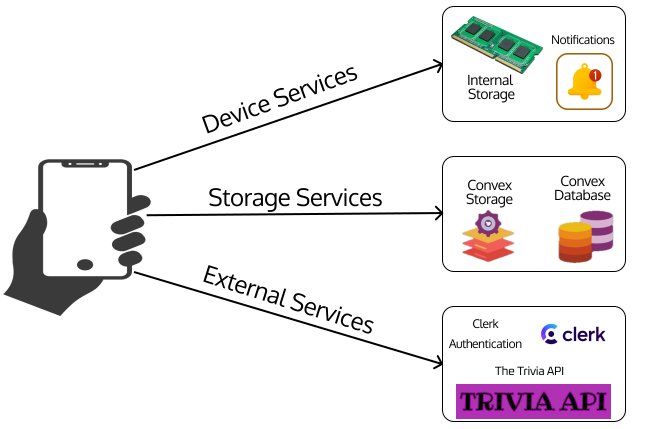
\includegraphics[width=1\textwidth, height=0.4\textheight]{Images/Application Architecture.png}
\caption{Device, Storage, and External Services Integration}
\end{figure}

\subsection{MVC Model: }

The Model represents the data layer of the application, encompassing both the data and the business logic. It is responsible for:

\begin{itemize}

    \item \textbf{Defining Data Structures:} The Model classes structure the data and define the attributes and relationships between different data entities.
    \item \textbf{Business Logic:} The Model contains the logic for data manipulation, validation, and rules enforcement. This ensures that the data remains consistent and accurate.
    \item \textbf{Data Persistence:} The Model interacts with storage services (internal storage and Convex Database) to persist and retrieve data.
\end{itemize}

\subsubsection{The View:}

The View is responsible for presenting the data to the user and handling user interaction. It includes the UI components such as buttons, forms, lists, and displays. The View:

\begin{itemize}

    \item \textbf{Renders the UI:} Displays data from the Model to the user in a readable and interactive format.
    \item \textbf{Receives User Input:} Captures user actions and inputs, such as clicks, typing, and selections.
    \item \textbf{Updates Dynamically:} Reflects changes in the Model by updating the displayed data without reloading the entire page.

\end{itemize}

\subsubsection{The Controller:}

The Controller acts as an intermediary between the Model and the View. It processes user inputs from the View, interacts with the Model to perform actions, and updates the View accordingly. The Controller:

\begin{itemize}

    \item \textbf{Handles User Inputs:} Captures events like button clicks, form submissions, and other user interactions.
    \item \textbf{Manipulates Data:} Calls Model methods to manipulate data based on user actions, ensuring the business logic is executed correctly.
    \item \textbf{Updates the View:} Ensures the View reflects the current state of the Model after data changes or actions.

\end{itemize}

\begin{figure}[H]
\centering
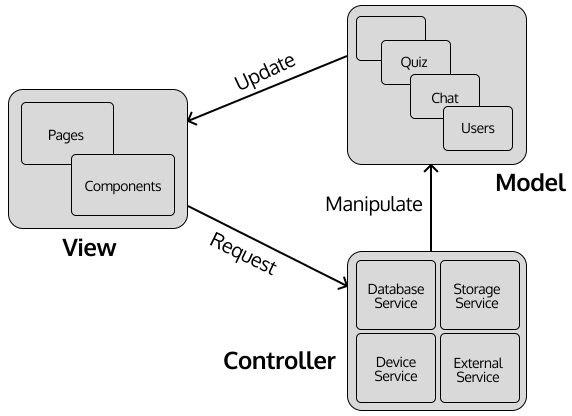
\includegraphics[width=0.8\textwidth]{Images/MVC Pattern.png}
\caption{Model-View-Controller (MVC) Pattern}
\end{figure}

\subsection{Device Services}

Device services in BrainMe include functionalities that are directly related to the device's capabilities:
\begin{enumerate}
\item \textbf{Internal Storage:} Used for storing user data locally on the device, ensuring quick access and offline capabilities.
\item \textbf{Notification:} Handles push notifications to keep users informed about updates, new quizzes, messages, and other relevant events.
\end{enumerate}

\subsection{Storage Services}

Storage services are crucial for data persistence and retrieval:
\begin{enumerate}
\item \textbf{Internal Storage:} Utilized for storing user preferences and other important data locally.
\item \textbf{Convex Database:} Serves as the primary database for storing structured data related to users, quizzes, messages, and leaderboard information.
\end{enumerate}

\subsection{External Services}

External services extend the functionality of BrainMe by integrating third-party APIs:
\begin{enumerate}
\item \textbf{Clerk Authentication:} Manages user authentication processes, including email/password logins and Single Sign-On (SSO) via Google and Apple.
\item \textbf{The Trivia API:} Provides quiz questions categorized by genre and level to enhance the learning experience.
\end{enumerate}

\subsection{Data Model}

Data shown in the application pages has been structured using classes which represent the Model part of the MVC pattern. The following objects are defined to structure the data appropriately:
\begin{enumerate}
\item \textbf{UserModel:} Contains information about registered users, including personal details and preferences.
\item \textbf{QuizModel:} Stores information about quizzes, including genre, level, and associated questions provided by The Trivia API.
\item \textbf{LeaderboardModel:} Tracks user performance and rankings within the application.
\item \textbf{MessageModel:} Contains attributes for messages sent and received within the app’s chat functionality.
\item \textbf{StatisticsModel:} Contains the detailed statistics such as points, correct answers ration, level, games played and so on.
\item \textbf{ChatModel:} Contains the detailed information about the users interacting with each other such as name, chats and the time stamp of when the message was sent and received.

\end{enumerate}

Data is fetched from different sources and is parsed using utility functions to obtain the desired structure. This ensures that the data presented in the application is accurate and up-to-date.
\section{Data Management}

\subsection{Data Storage}

\subsubsection{Convex Database}

The Convex database is the main storage solution for BrainMe. It stores all structured data related to users, quizzes, messages, and leaderboard information. The database schema is designed to ensure efficient data retrieval and management.

\begin{itemize}
  \item \textbf{Users Collection:} The users collection stores information about registered users, including their email, username, and profile picture URL. Profile pictures are stored in cloud storage. Other fields include friends list and file storage for user-uploaded files. Sub-collections store references to quizzes and messages the user is involved in.
  \item \textbf{Quizzes Collection:} Quizzes from The Trivia API are stored in the Convex database. This collection includes quiz categories, difficulty levels, individual questions, and answers. Each quiz document links to the relevant user who created or participated in the quiz.
  \item \textbf{Messages Collection:} The messages collection stores all chat messages exchanged within the application. Each message document includes the sender's reference, the content of the message, and a timestamp.
  \item \textbf{Statistics Collection:} The statistics collection stores all information related to user statistics including the number of correct answers, the points the user has earned to date, the user level, and the number of games played.
  \item \textbf{Chat Collection:} The chat collection stores information about each chat, including the participants, the last comment made, and the timestamp of the last activity.
  \item \textbf{Leaderboard Collection:} The leaderboard collection stores information about user rankings and points. This collection includes user IDs, the points each user has earned, and their ranking position.
\end{itemize}

\subsection{Cloud Storage}

\subsubsection{Profile Pictures and Attachments}

Cloud storage is used to store user-generated content such as profile pictures and attachments uploaded. The structure of the storage is organized by user IDs to ensure easy retrieval and management.

\subsubsection{Storage Structure}

The main folders in cloud storage include:

\begin{enumerate}
\item \textbf{Profile Pictures:} Each user has a unique profile picture stored in this folder.
\item \textbf{Avatars:} Predefined avatars are stored in separate folders.
\end{enumerate}

\subsection{Shared Preferences}

\subsubsection{Local Storage for Preferences}

Shared preferences provide persistent storage for simple data in a key-value format on the device's memory. This is used to store user preferences such as:

\begin{enumerate}
\item \textbf{Notification Settings:} Users can enable or disable chat notifications (keys: notificationChat).
\end{enumerate}

\subsection{External Services}

\subsubsection{Clerk Authentication}

Clerk manages user authentication, supporting email/password logins and Single Sign-On (SSO) with Google, Facebook and Apple. It stores user credentials and ensures secure access to the application.

\subsubsection{The Trivia API}

The Trivia API provides a vast collection of quiz questions. These questions are categorized by genre and difficulty level, and are stored in the Convex database for use in the quiz-based learning feature.

\subsection{Local Storage}

\subsubsection{File Upload and Download}

One of the key features of BrainMe is the ability to upload and view attachments. Users can upload various file types (e.g., PDFs, images) from their device's local storage. Public notes and attachments can be downloaded by other registered users for offline access.

\subsection{Dependencies}

\begin{longtable}{|p{4cm}|p{10cm}|}
\hline
\textbf{Package Name} & \textbf{Functionality} \\
\hline
@clerk/clerk-expo & Provides Clerk integration for Expo applications, enabling secure user authentication. \\
\hline
@clerk/clerk-react & Provides Clerk integration for React applications, enabling secure user authentication. \\
\hline
@expo-google-fonts/pacifico & Offers the Pacifico font from Google Fonts, ensuring consistent typography. \\
\hline
@expo/vector-icons & A set of vector icons for React Native, useful for enhancing the UI with icons. \\
\hline
@react-navigation/native & Manages navigation within the application, supporting multiple navigation patterns. \\
\hline
convex & Serves as the backend database, storing all structured data. \\
\hline
expo & The core Expo SDK, providing essential tools and services for Expo projects. \\
\hline
expo-constants & Accesses system information such as device ID and app version. \\
\hline
expo-font & Manages custom fonts in Expo applications. \\
\hline
expo-image-picker & Allows users to pick images from their device's library or camera. \\
\hline
expo-linking & Handles deep linking in Expo applications. \\
\hline
expo-router & Handles seamless navigation within the application. \\
\hline
expo-secure-store & Provides a way to securely store sensitive information. \\
\hline
expo-splash-screen & Manages the splash screen, showing it while the app is loading. \\
\hline
expo-status-bar & Manages the appearance of the status bar. \\
\hline
expo-system-ui & Allows control over the system UI, such as the status bar and navigation bar. \\
\hline
expo-web-browser & Enables opening URLs in the system's web browser. \\
\hline
react & A JavaScript library for building user interfaces. \\
\hline
react-dom & Serves as the entry point to the DOM and server renderers for React. \\
\hline
react-native & Framework for building natively compiled applications for mobile platforms using JavaScript and React. \\
\hline
react-native-gesture-handler & Provides native gesture handling capabilities for React Native apps. \\
\hline
react-native-get-random-values & Polyfill for the getRandomValues function, enabling secure random number generation. \\
\hline
react-native-reanimated & Enables complex animations in React Native applications. \\
\hline
react-native-safe-area-context & Manages safe area boundaries in React Native applications. \\
\hline
react-native-screens & Optimizes navigation by using native screen components. \\
\hline
react-native-web & Enables React Native components to be used in web applications. \\
\hline
\end{longtable}

\subsection{Components Architecture}

The architecture of the app is designed to work seamlessly on both tablets and iOS mobile screens. We use responsive design principles to ensure a consistent user experience across different devices. The layout adapts to various screen sizes, providing an optimal viewing and interaction experience.

\begin{itemize}
    \item \textbf{Presentation Layer:} This layer is where users interact with the app. It includes:
    \begin{itemize}
        \item \textit{RegistrationScreen}: Where users sign up.
        \item \textit{LoginScreen}: Where users log in.
        \item \textit{ProfileScreen}: Where users view and edit their profile.
        \item \textit{QuizInterface}: Where users take quizzes.
        \item \textit{QuizSelectionScreen}: Where users select quiz topics.
        \item \textit{LeaderboardScreen}: Where users see rankings.
        \item \textit{MessagingInterface}: Where users send and receive messages.
    \end{itemize}

         \item \textbf{Business Logic Layer:} This layer handles the main functions and rules of the app. It includes:
        \begin{itemize}
            \item \textit{UserModel}: Manages user data.
            \item \textit{StatisticsModel}: Tracks user statistics.
            \item \textit{QuizModel}: Manages quiz data.
            \item \textit{LeaderboardModel}: Manages leaderboard data.
            \item \textit{ChatModel}: Manages chat data.
            \item \textit{MessageModel}: Manages messages.
        \end{itemize}

\begin{figure}[H]
    \centering
    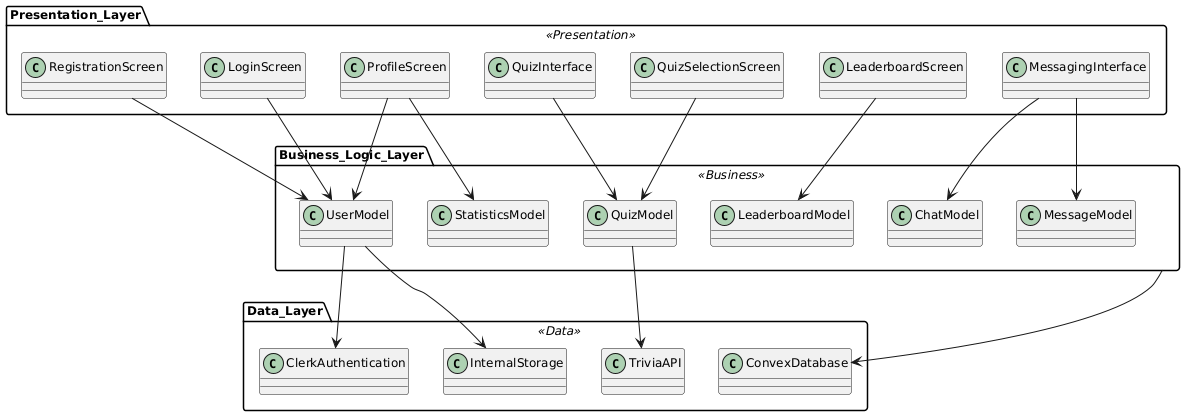
\includegraphics[width=1.1\linewidth, height=0.4\textheight]{Images/Components Architecture.png}
    \caption{Layered Architecture}
\end{figure}


    \item \textbf{Data Layer:} This layer handles storing and retrieving data. It includes:
    \begin{itemize}
        \item \textit{ClerkAuthentication}: Manages user logins.
        \item \textit{InternalStorage}: Stores data on the device.
        \item \textit{TriviaAPI}: Provides quiz questions.
        \item \textit{ConvexDatabase}: Stores structured data.
    \end{itemize}
\end{itemize}

The layers are linked like this: 

\begin{itemize}
     
    \item The \textbf{Presentation Layer} shows data to users and gets their inputs.
    \item The \textbf{Business Logic Layer} processes this data and applies the app’s rules.
    \item The \textbf{Data Layer} stores and retrieves the data when needed.
\end{itemize}

For example, when a user logs in (Presentation Layer), the login details are sent to the \textit{UserModel} (Business Logic Layer), which checks the details with \textit{ClerkAuthentication} (Data Layer). If the login is successful, the user's profile data is retrieved from the \textit{ConvexDatabase} (Data Layer) and displayed on the \textit{ProfileScreen} (Presentation Layer). \\\\
This setup makes it easy to manage and update the app. Each layer does its specific job, making the app work smoothly.

\subsection{Class Diagrams}

Class diagrams played a crucial part of the design and architecture of our BrainMe mobile application. They visually represent the structure of the system by showing the system's classes, their attributes, and the relationships among objects. This helped us in understanding how data is managed within the application, ensuring that the data remains organized and non-redundant.

\begin{figure}[H]
    \centering
    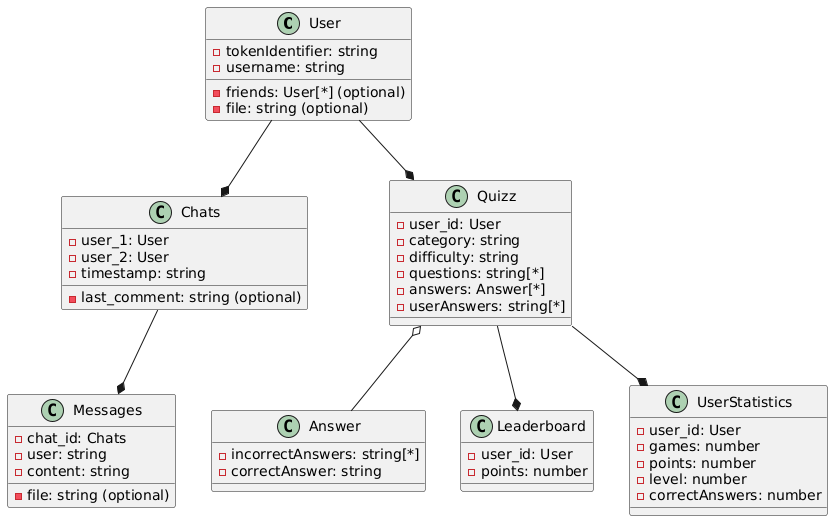
\includegraphics[width=1\linewidth, height=0.4\textheight]{Images/class diagram.png}
    \caption{Class Diagram}
\end{figure}

The above class diagram illustrates the main components of the BrainMe application:

\begin{itemize}
    \item \textbf{User:} Represents a user in the system. Each user has attributes like `tokenIdentifier`, `username`, a list of friends (`friends`), and an optional `file`.
    
    \item \textbf{Chats:} Represents a chat session between two users. It includes the `user\_1` and `user\_2` involved in the chat, the timestamp of the chat, and an optional `last\_comment`.
    
    \item \textbf{Messages:} Represents the individual messages within a chat. It contains the `chat\_id` it belongs to, the `user` who sent it, the `content` of the message, and an optional `file`.
    
    \item \textbf{Leaderboard:} Represents the leaderboard data. It includes `user\_id` and `points`.
    
    \item \textbf{Quiz:} Represents the quiz data associated with a user. It includes `user\_id`, `category`, `difficulty`, a list of `questions`, a list of `answers` (which includes `incorrectAnswers` and `correctAnswer`), and a list of `userAnswers`.
    
    \item \textbf{UserStatistics:} Represents the statistics for a user. It includes `user\_id`, `games`, `points`, `level`, and `correctAnswers`.
\end{itemize}

\textbf{The relationships between these classes are as follows:}

\begin{itemize}
    \item A \textbf{User} can have multiple \textbf{Chats} and can send multiple \textbf{Messages}.
    \item Each \textbf{Chat} contains multiple \textbf{Messages}.
    \item A \textbf{User} is ranked in the \textbf{Leaderboard}.
    \item A \textbf{User} can participate in multiple \textbf{Quizzes}.
    \item A \textbf{Quiz} contains multiple \textbf{Answers}.
\end{itemize}

\textbf{Importance and Benefits:}
\begin{itemize}
    \item \textbf{Data Organization:} The class diagram ensures that the data is structured logically, making it easier to manage and retrieve information.
    \item \textbf{Non-redundant Data:} By clearly defining the relationships and dependencies, the diagram helps in avoiding data redundancy.
    \item \textbf{Clear Understanding:} It provides a clear visual representation of the system's structure, aiding developers and stakeholders in sunderstanding the system's functionality.
    \item \textbf{Efficient Development:} With a well-defined class diagram, we were able to follow a structured approach to build and expand the application.
\end{itemize}

\subsection{Sequence Diagrams}

Sequence diagrams offer a visual representation of how different components or objects interact and cooperate within our system; these diagrams provide a clear understanding of the system's behavior, communication patterns, and the responsibilities of each element. For these reasons, the sequence diagram of the most relevant actions of our application is shown.

\subsubsection{LogIn}

\begin{figure}[H]
    \centering
    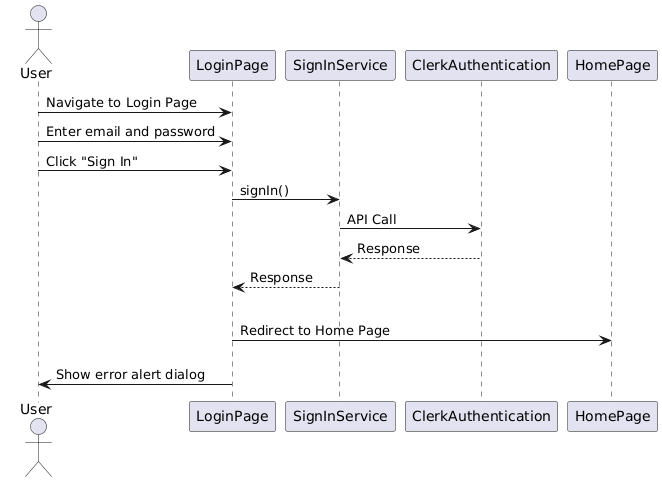
\includegraphics[width=1\linewidth, height=0.4\textheight]{Sequence Diagrams/Login.png}
    \caption{Login Sequence Diagram}
\end{figure}

The sequence diagram for the login process in the BrainMe application is explained as follows:

\begin{itemize}
    \item The user starts by opening the login page and entering their email and password into the respective form fields.
    \item Upon submitting the login form, the `SignIn()` method is called, which sends the login credentials to the SignIn Service.
    \item The SignIn Service then makes an API call to the Clerk Authentication service to validate the provided credentials.
    \item Clerk Authentication processes the request and sends a response back to the SignIn Service, indicating whether the credentials are valid or not.
    \item The SignIn Service forwards the response to the login page.
    \item An alternative path is defined based on the validity of the credentials:
    \begin{itemize}
        \item If the credentials are correct, the user is redirected to the home page using the `Go to Home Page()` method.
        \item If the credentials are incorrect, an error alert dialog is shown to the user, indicating that the login attempt was unsuccessful.
    \end{itemize}
\end{itemize}

\subsubsection{Chat System}

\begin{figure}[H]
    \flushleft
    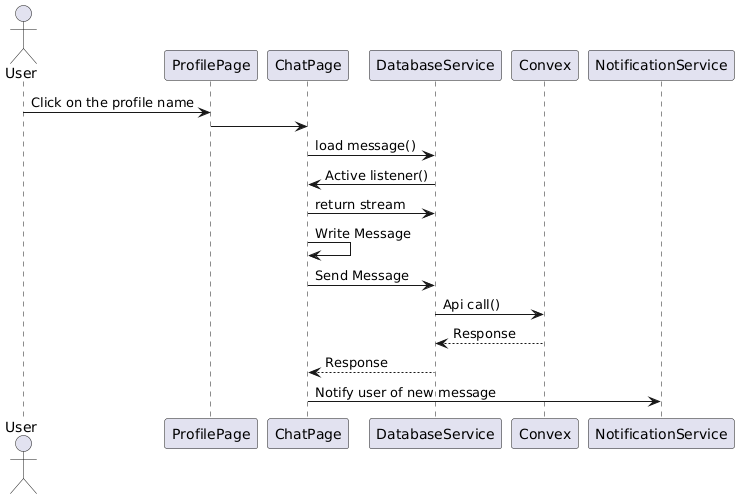
\includegraphics[width=1\linewidth, height=0.4\textheight]{Sequence Diagrams/Chat System.png}
    \caption{Chat System Sequence Diagram}
\end{figure}
The sequence diagram for the message system in the BrainMe application is explained as follows:

\begin{itemize}
    \item The user starts by clicking on a profile name from the profile page to initiate a chat.
    \item This action loads the chat page and triggers the `load message()` function, which requests messages from the Database Service.
    \item The Database Service sets up an active listener to stream messages back to the chat page.
    \item The stream of messages is returned to the chat page, allowing the user to see the conversation history.
    \item The user writes a message in the chat interface and sends it.
    \item The `Send Message` action is called, which sends the message to the Database Service.
    \item The Database Service makes an API call to Convex to store the message.
    \item Convex processes the request and sends a response back to the Database Service.
    \item The Database Service sends a notification to the Notification Service.
    \item The Notification Service notifies the user of the new message.
\end{itemize}

\subsubsection{Leaderboard}

The sequence diagram for the leaderboard process in the BrainMe application is explained as follows:

\begin{itemize}
    \item The user starts a quiz from the QuizPage, which directly requests quiz questions from the TriviaAPI.
    \item The TriviaAPI returns the quiz questions to the QuizPage.
    \item The user submits their answers, which are sent to the BackendServices.
    \item BackendServices validate and store the results in the ConvexDatabase.
    \item ConvexDatabase sends a store confirmation back to BackendServices.
    \item BackendServices update the user's points and progress and subsequently update the leaderboard.
    \item The updated leaderboard information is confirmed back to BackendServices.
    \item BackendServices send a submission confirmation to the QuizPage.
    \item The QuizPage then notifies the user of their results via the NotificationService.
\end{itemize}


\begin{figure}[H]
    \centering
    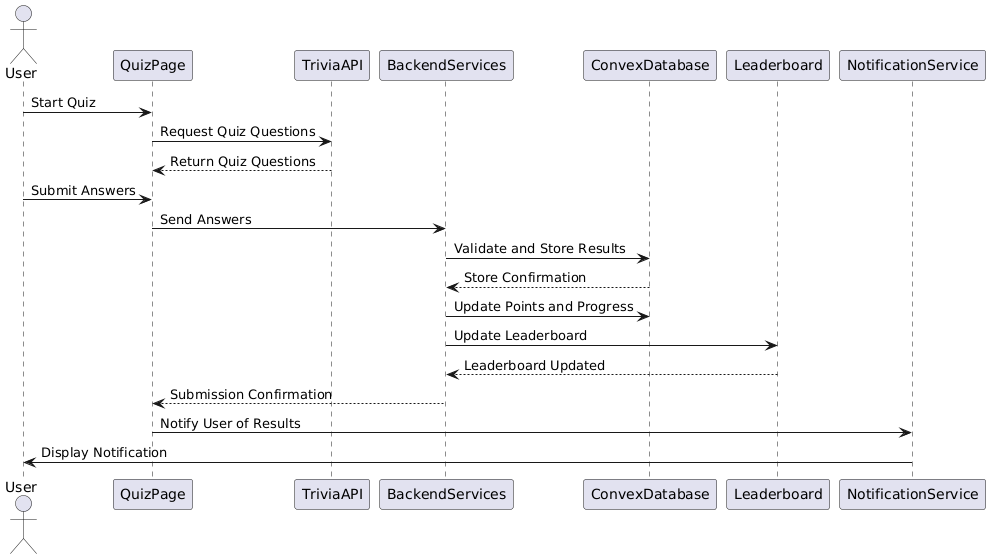
\includegraphics[width=1\linewidth, height=0.5\textheight]{Sequence Diagrams/leaderboard.png}
    \caption{Leaderboard Sequence Diagram}
\end{figure}



\subsubsection{Quiz Review}

The sequence diagram for the quiz review process in the BrainMe application is explained as follows:

\begin{itemize}
    \item The user completes a quiz and the Quiz Page stores the quiz results in the Convex Database.
    \item The Convex Database sends a store confirmation back to the Quiz Page.
    \item The Quiz Page shows the user an option to review the quiz immediately or go back to the home page.
    \item If the user chooses to review the quiz immediately:
    \begin{itemize}
        \item The user selects the review quiz option.
        \item The Quiz Page requests quiz details and answers from the Convex Database.
        \item The Convex Database returns the quiz details, answers, and explanations to the Quiz Page.
        \item The Quiz Page displays the quiz details, answers, and explanations to the user.
    \end{itemize}
    \item If the user chooses to go back to the home page, they are redirected there.
    \item If the user does not choose to review the quiz immediately, no review option is available later.
\end{itemize}

\begin{figure}[H]
    \centering
    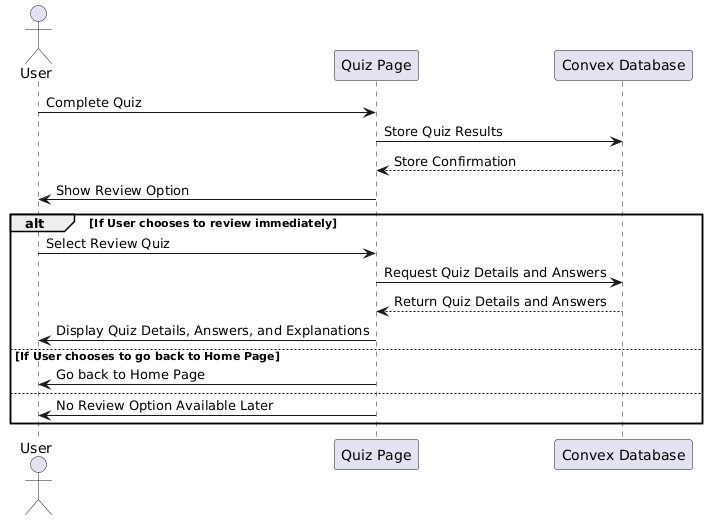
\includegraphics[width=1\linewidth, height=0.52\textheight]{Sequence Diagrams/Quiz Review.png}
    \caption{Quiz Review Sequence Diagram}
\end{figure}


\subsubsection{Profile Update}

The sequence diagram for the profile update process in the BrainMe application is explained as follows:

\begin{itemize}
    \item The user navigates to the Profile Page and makes changes to their profile.
    \item The Profile Page sends the updated data to Backend Services.
    \item Backend Services validate and update the user data in Convex Database.
    \item Backend Services confirm the update.
    \item The updated profile information is reflected on the Profile Page.
\end{itemize}


\begin{figure}[H]
    \centering
    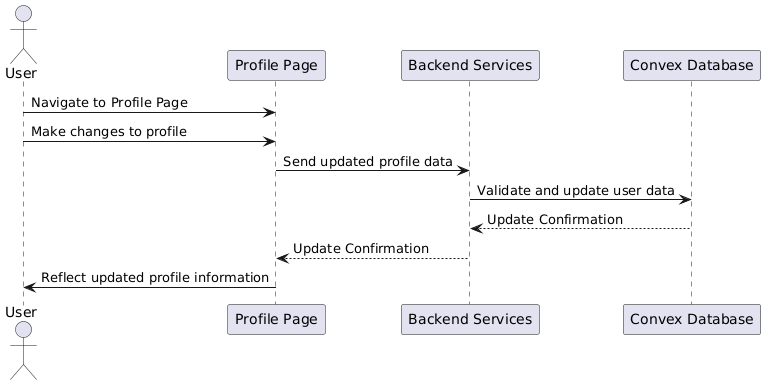
\includegraphics[width=1\linewidth, height=0.4\textheight]{Sequence Diagrams/profile update.png}
    \caption{Profile Update Sequence Diagram}
\end{figure}

\subsubsection{LogOut}

\begin{itemize}
    \item The user navigates to the Logout Page.
    \item The user clicks "Sign Out".
    \item The Logout Page calls the `signOut()` method in the Sign Out Service.
    \item The Sign Out Service makes an API call to Clerk Authentication.
    \item Clerk Authentication processes the request and sends a response back to the Sign Out Service.
    \item The Sign Out Service forwards the response to the Logout Page.
    \item An alternative path is defined based on the success of the logout:
    \begin{itemize}
        \item If logout is successful, the user is redirected to the Authentication Page.
        \item If logout fails, an error alert dialog is shown to the user.
    \end{itemize}
\end{itemize}

\begin{figure}[H]
    \centering
    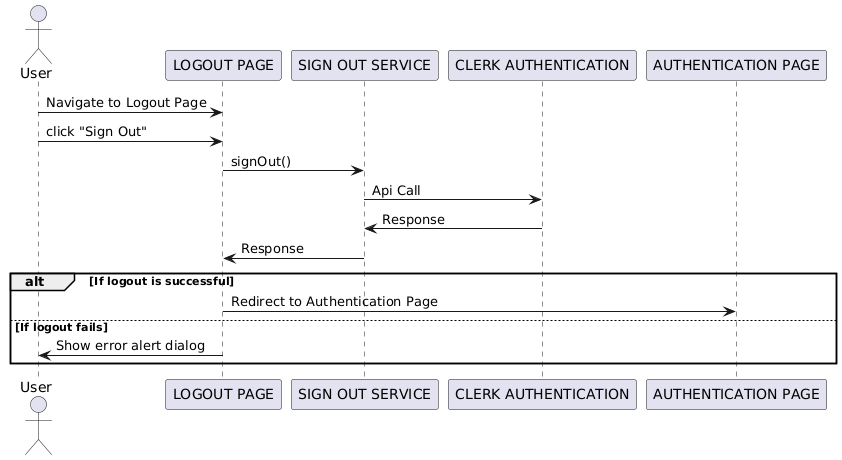
\includegraphics[width=1\linewidth, height=0.5\textheight]{Sequence Diagrams/logout.png}
    \caption{Logout Sequence Diagram}
\end{figure}

The sequence diagram for the logout process in the BrainMe application is explained as follows:



\subsection{Gamification}

Gamification plays a significant role in enhancing user engagement and motivation in the BrainMe application. Here is how it is implemented:

\textbf{Points System:}
\begin{itemize}
    \item Completing an easy quiz earns the user 2 points.
    \item Completing a medium quiz earns the user 3 points.
    \item Completing a hard quiz earns the user 5 points.
\end{itemize}

\textbf{General Formula: }

\begin{itemize}
    \item For any \textbf{level $n$}: \\
    $L_n = 10 \times 2^{(n-1)}$
\end{itemize}

\textbf{Level Progression:}
\begin{itemize}
    \item \textbf{Level 1:} \\
    $L_1 = 0$
    \item \textbf{Level 1 to Level 2:} \\
    $L_{1\rightarrow2} = 10 \times 2^1 = 10$
    \item \textbf{Level 2 to Level 3:} \\
    $L_{2\rightarrow3} = 10 \times 2^2 = 20$
    \item \textbf{Level 3 to Level 4:} \\
    $L_{3\rightarrow4} = 10 \times 2^3 = 40$
    \item \textbf{Level 4 to Level 5:} \\
    $L_{4\rightarrow5} = 10 \times 2^4 = 80$
\end{itemize}


\textbf{Medals and Rewards:}
\begin{itemize}
    \item Users who achieve the top 3 ranks on the leaderboard receive special Medals.
    \item These Medals are displayed on their profiles to acknowledge their achievements and motivate other users.
\end{itemize}

This gamification strategy not only encourages users to actively participate in quizzes and improve their knowledge but also fosters a sense of achievement and competition among users.

\section{User Interface (UI)}
The User Interface (UI) of BrainMe is designed with a focus on simplicity, usability, and engagement. We aim to create an intuitive and visually appealing interface that enhances the overall user experience. By adhering to best practices in UI design and incorporating feedback from users, we ensure that the app is both functional and aesthetically pleasing.

\subsection{UI Design Choices}

The UI design choices for BrainMe are centered around creating a seamless and enjoyable user experience. This includes selecting appropriate color schemes, typography, and layout structures that facilitate easy navigation and interaction.

\subsubsection{User Interaction}

User interaction is at the core of BrainMe's design philosophy. The app employs intuitive touch gestures and responsive controls to make it easy for users to navigate through the various features. Buttons, icons, and interactive elements are designed to be easily accessible and recognizable, reducing the learning curve for new users. Feedback mechanisms, such as animations and visual cues, are used to provide immediate responses to user actions, ensuring a smooth and engaging experience.


\subsubsection{Main Design}

The main design of BrainMe is clean and modern, with a focus on clarity and ease of use. The layout is structured to minimize clutter and highlight the most important elements on each screen. Consistent use of colors, fonts, and spacing helps create a cohesive visual experience. The design also incorporates accessibility features, such as adjustable text sizes and high-contrast modes, to ensure that the app is usable by people with diverse needs and preferences.


\subsection{Smartphone UI}

The smartphone UI for BrainMe is optimized for small screens, ensuring that all features are easily accessible and usable on mobile devices. The interface is designed to be responsive, adapting to different screen sizes and orientations to provide a consistent experience across all devices.


\subsubsection{Login and Registration}

The login and registration screens are designed to be simple and straightforward, allowing users to quickly access the app. Clear input fields, helpful instructions, and error messages guide users through the process. Options for signing in with email, Google, or Apple are prominently displayed, making it easy for users to choose their preferred method. The design ensures that users can complete the login or registration process with minimal effort and time.

\begin{figure}[H]
    \centering
    \begin{minipage}[b]{0.43\linewidth}
        \centering
        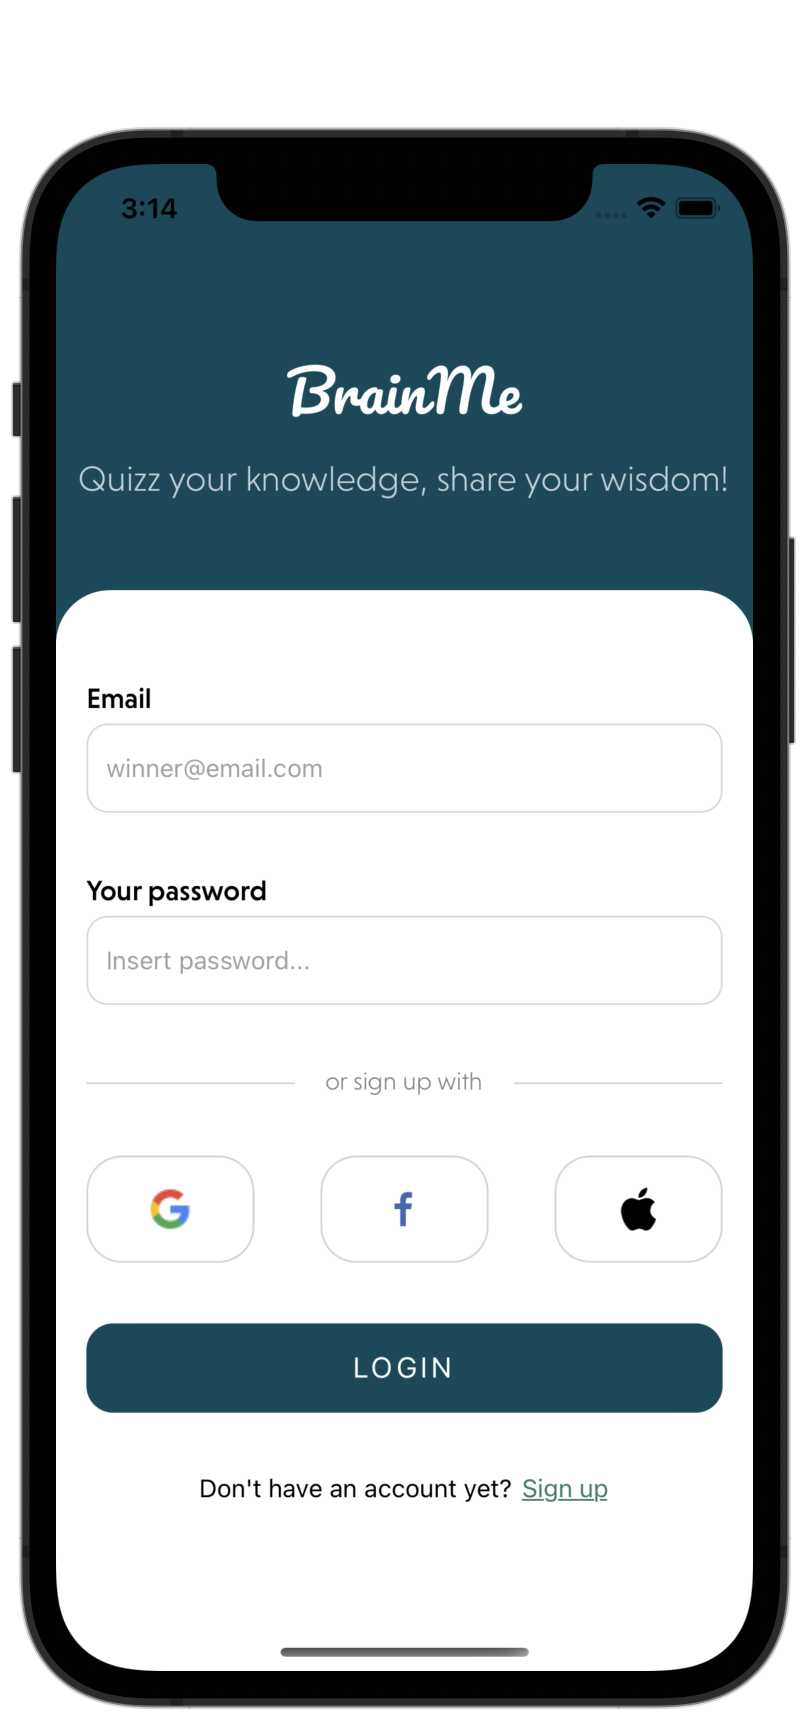
\includegraphics[width=\linewidth]{Mobile UI/Login.png}
        \caption{Login Page}
    \end{minipage}
    \hspace{0.1\linewidth}
    \begin{minipage}[b]{0.43\linewidth}
        \centering
        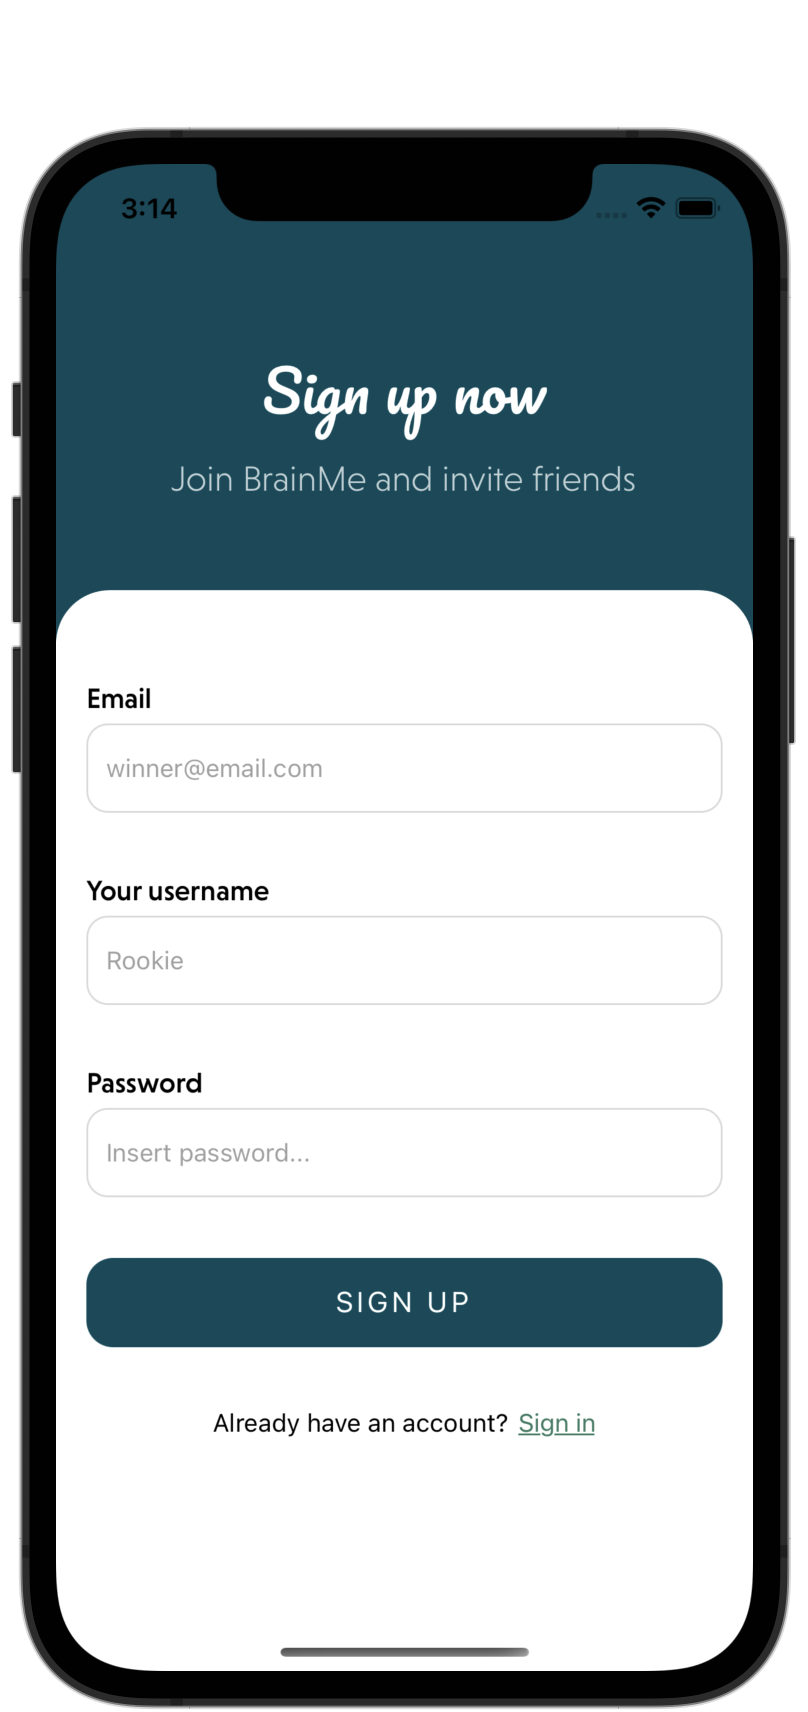
\includegraphics[width=\linewidth]{Mobile UI/Signup.png}
        \caption{Sign Up Page}
    \end{minipage}
    \vspace{0.5cm}
    \caption{\textbf{The BrainMe Application}}
\end{figure}

\subsubsection{Quiz Page: }

The quiz page provides users with a variety of quiz categories to choose from. The interface is designed to be engaging and user-friendly, with clearly labeled icons for each category. Users can easily navigate through different topics such as History, Geography, Music, Arts \& Literature, Science, General Knowledge, Sport, Food, Movie, and Culture. The page also displays the user's current level and progress towards the next level, motivating them to participate in more quizzes. The design ensures that users can quickly select their desired quiz category and start testing their knowledge immediately.

\begin{figure}[H]
    \centering
    \begin{minipage}[b]{0.43\linewidth}
        \centering
        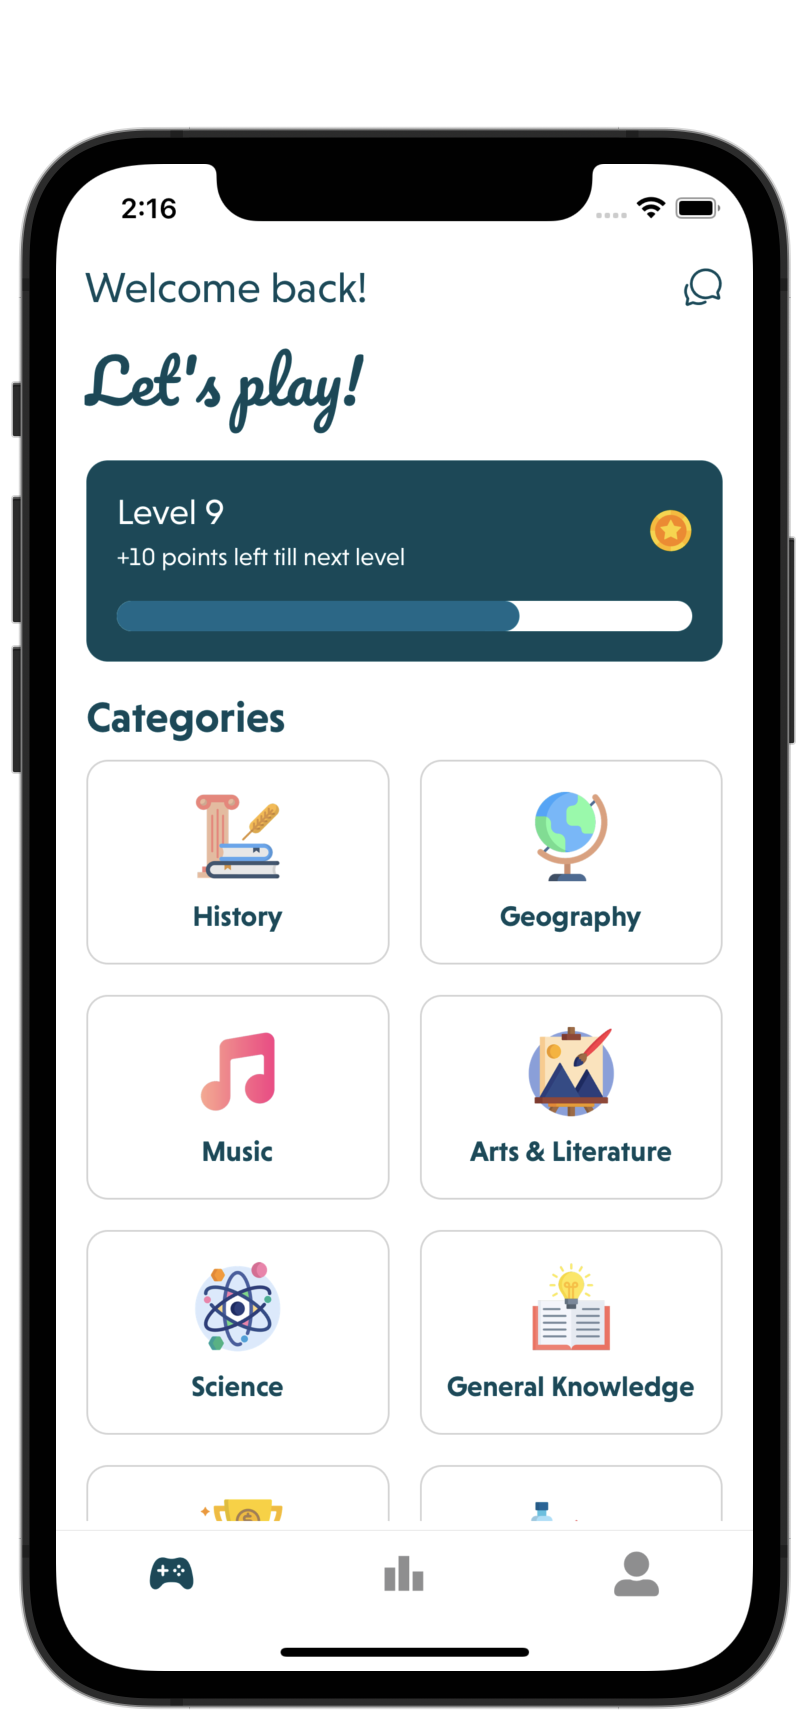
\includegraphics[width=\linewidth]{Mobile UI/Quiz Page 1.png}
        \caption{Quiz Page 1}
    \end{minipage}
    \hspace{0.1\linewidth}
    \begin{minipage}[b]{0.43\linewidth}
        \centering
        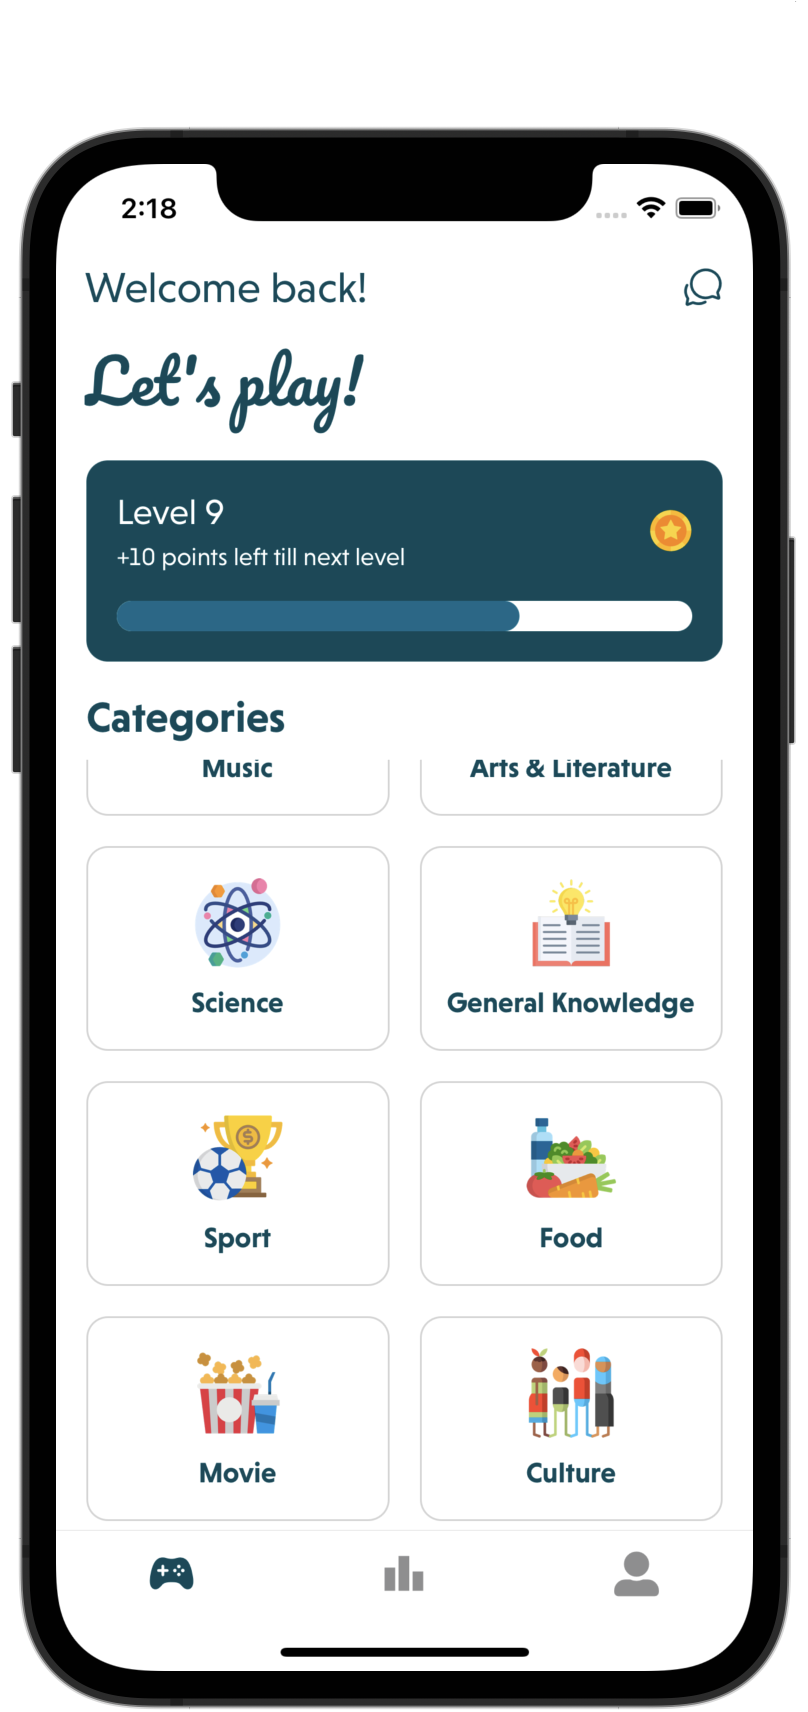
\includegraphics[width=\linewidth]{Mobile UI/Quiz Page 2.png}
        \caption{Quiz Page 2}
    \end{minipage}
    \vspace{0.5cm}
    \caption{\textbf{The BrainMe Application All Quiz Categories}}
\end{figure}


\subsubsection{Quiz Levels: }

The Quiz Levels screen allows users to select the difficulty level of the quiz they want to take. The interface is intuitive, with options for Easy, Medium, and Hard difficulties prominently displayed. Each difficulty level is accompanied by a brief description of what to expect, helping users choose the most suitable challenge. \\\\
The points distribution for each difficulty level is also provided, encouraging users to aim for higher scores by attempting more challenging quizzes. This screen ensures that users are well-informed about their choices and can customize their quiz experience according to their skill level and preferences. \\\\
Lastly, if the user tries to proceed without selecting any difficulty level as in the Figure 21, the user gets to see a message asking to select a difficulty level.

\begin{figure}[H]
    \centering
    \begin{minipage}[b]{0.43\linewidth}
        \centering
        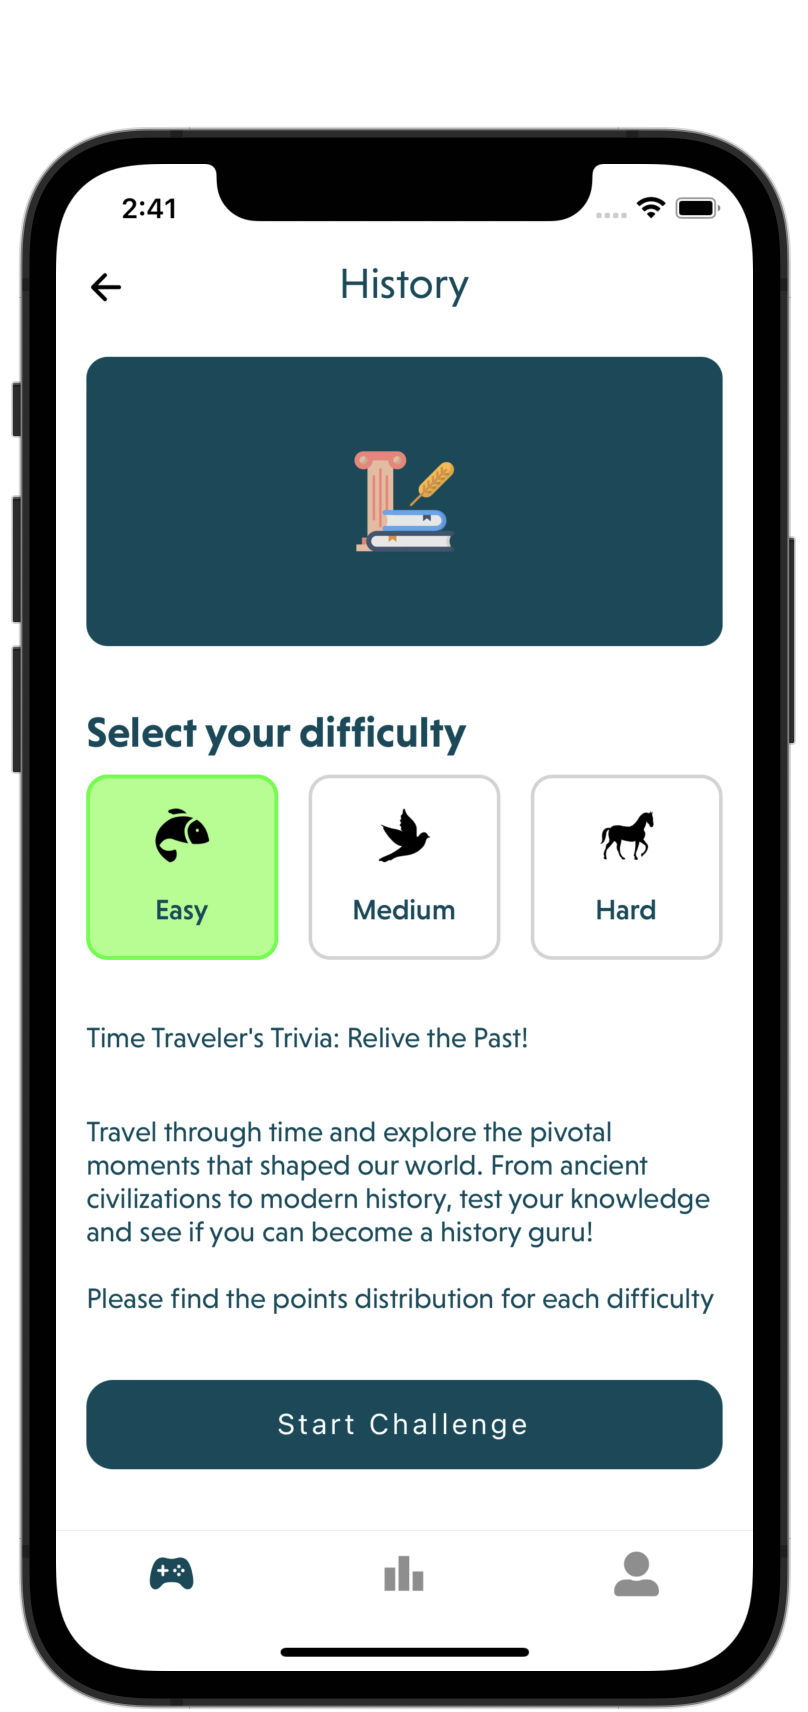
\includegraphics[width=\linewidth]{Mobile UI/Easy Level Quiz.png}
        \caption{Easy Level Quiz}
    \end{minipage}
    \hspace{0.1\linewidth}
    \begin{minipage}[b]{0.43\linewidth}
        \centering
        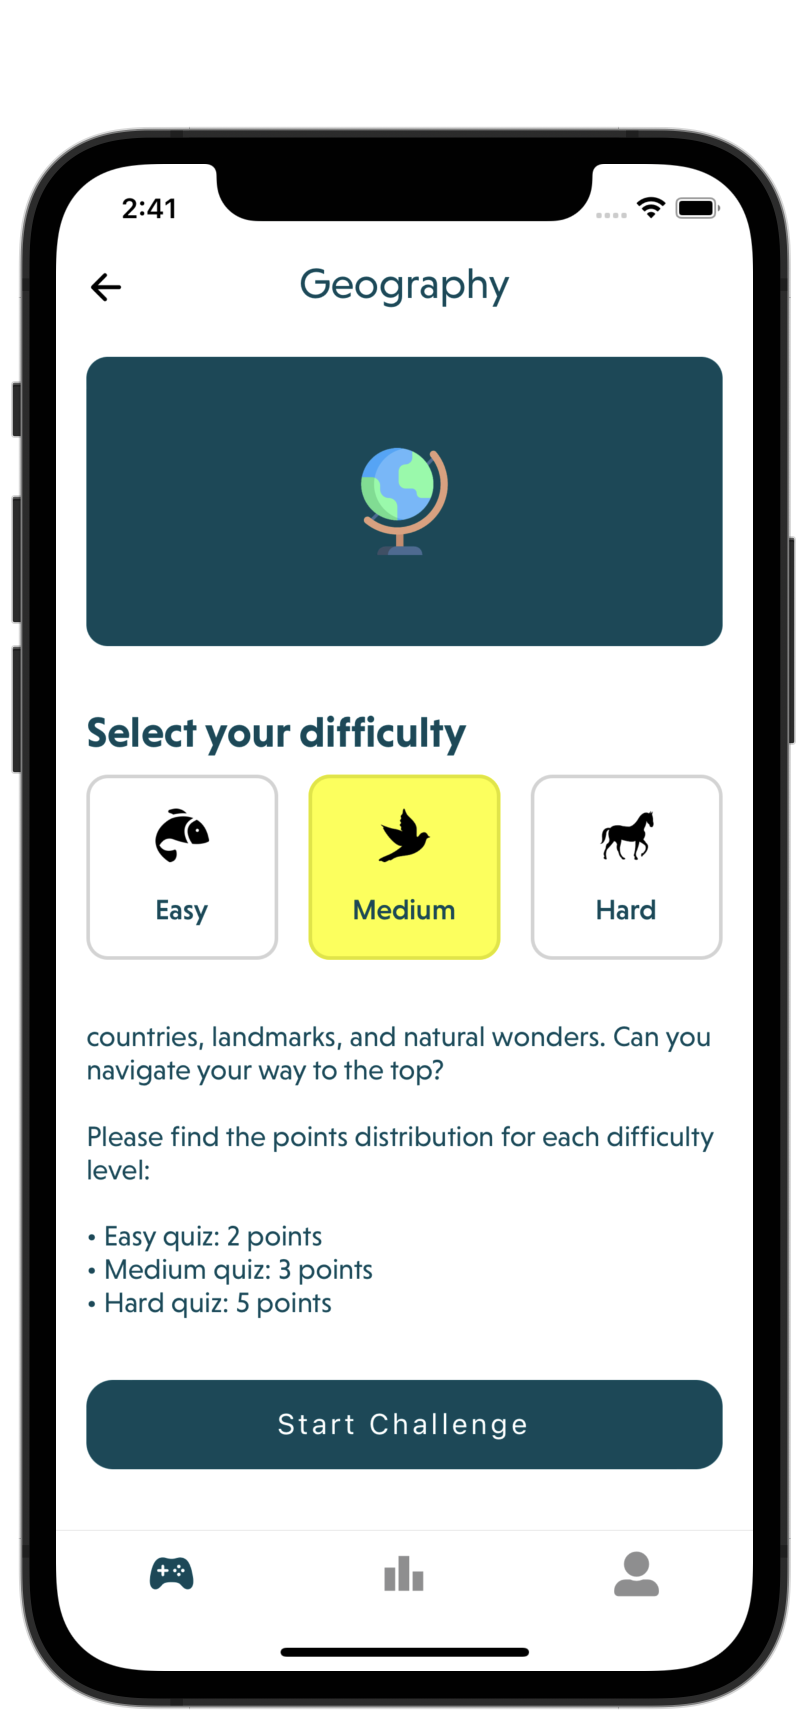
\includegraphics[width=\linewidth]{Mobile UI/Medium Level Quiz.png}
        \caption{Medium Level Quiz}
    \end{minipage}
    \vspace{0.5cm}
    \caption{\textbf{Quiz Difficulty Description}}
\end{figure}


\begin{figure}[H]
    \centering
    \begin{minipage}[b]{0.43\linewidth}
        \centering
        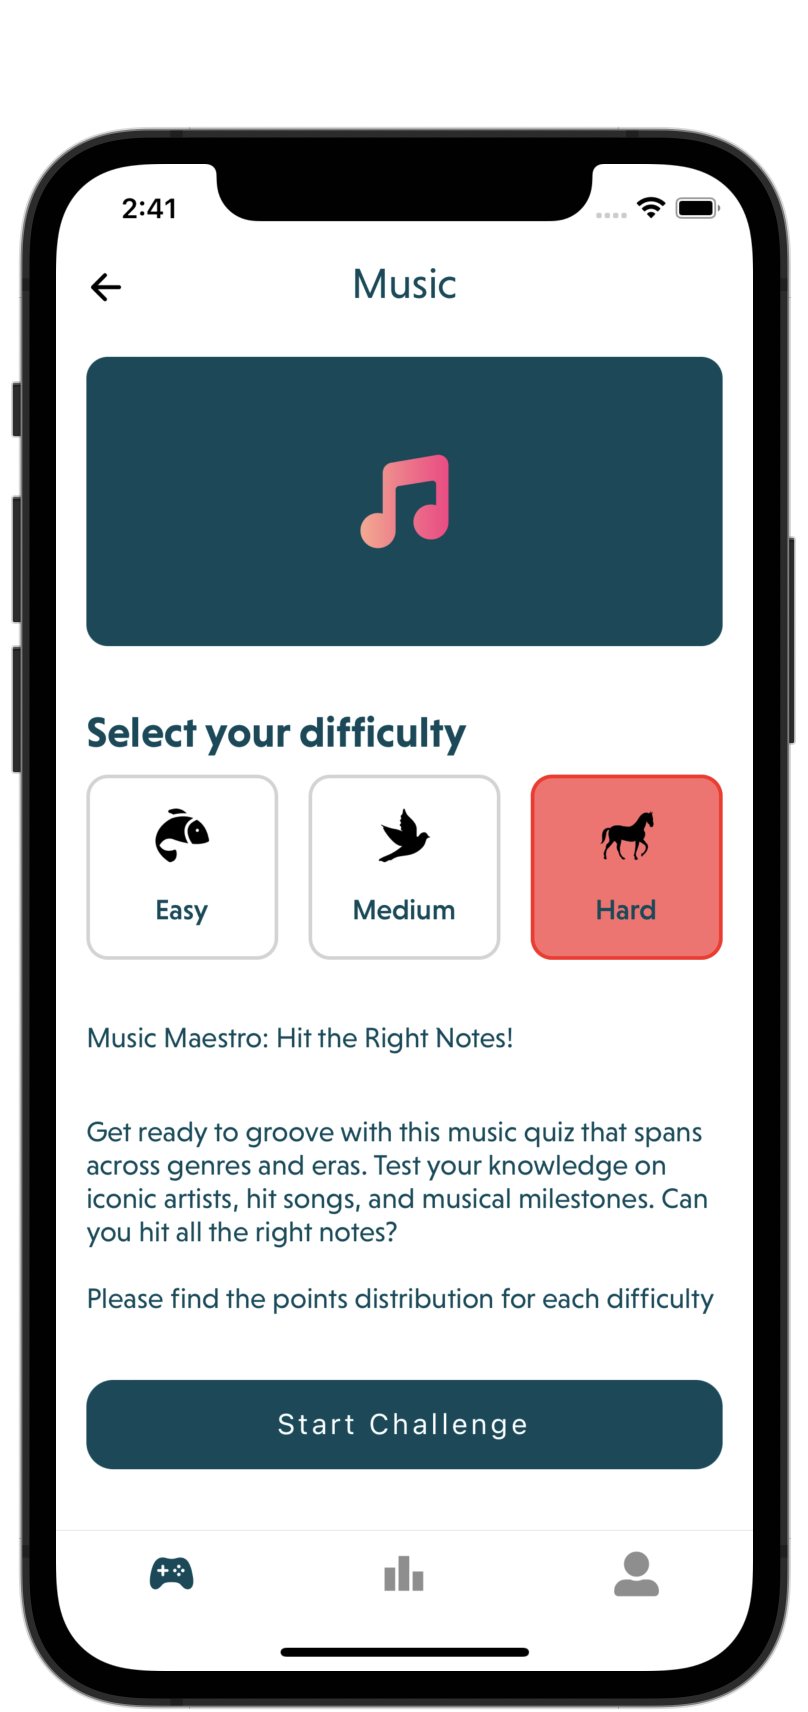
\includegraphics[width=\linewidth]{Mobile UI/Hard Level Quiz.png}
        \caption{Hard Level Quiz}
    \end{minipage}
    \hspace{0.1\linewidth}
    \begin{minipage}[b]{0.43\linewidth}
        \centering
        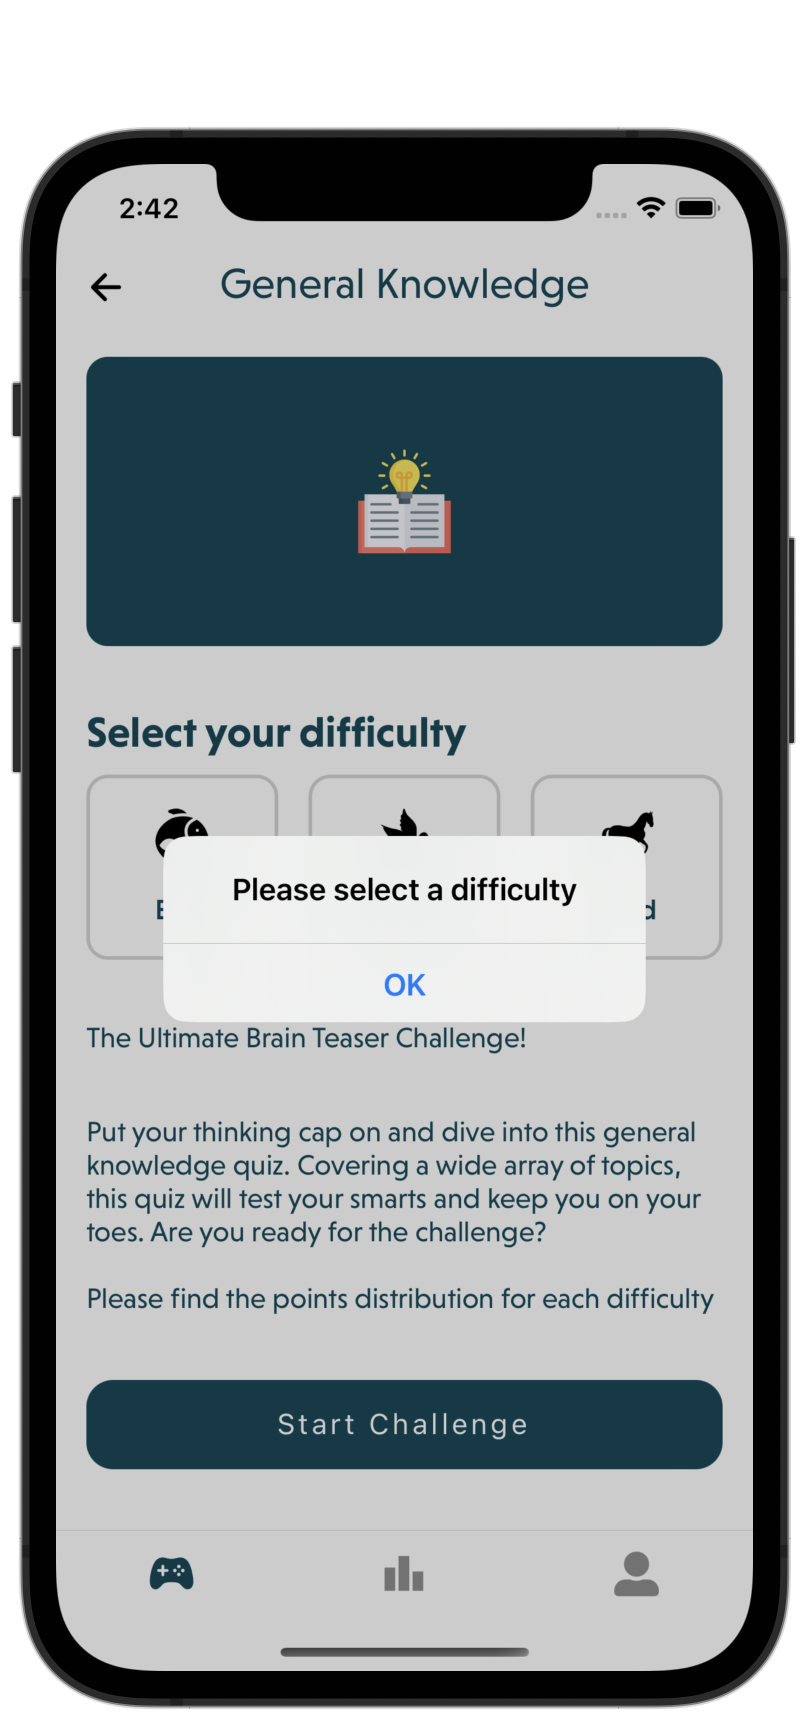
\includegraphics[width=\linewidth]{Mobile UI/Select Difficulty.png}
        \caption{Select Difficulty}
    \end{minipage}
    \vspace{0.5cm}
    \caption{\textbf{Quiz Difficulty Description}}
\end{figure}

\vspace{1cm}

\subsubsection{Starting Quiz}

The starting quiz screens guide users through the process of answering quiz questions. The design ensures that users can easily select their answers and see immediate feedback on their choices.

\begin{figure}[H]
    \centering
    \begin{minipage}[b]{0.43\linewidth}
        \centering
        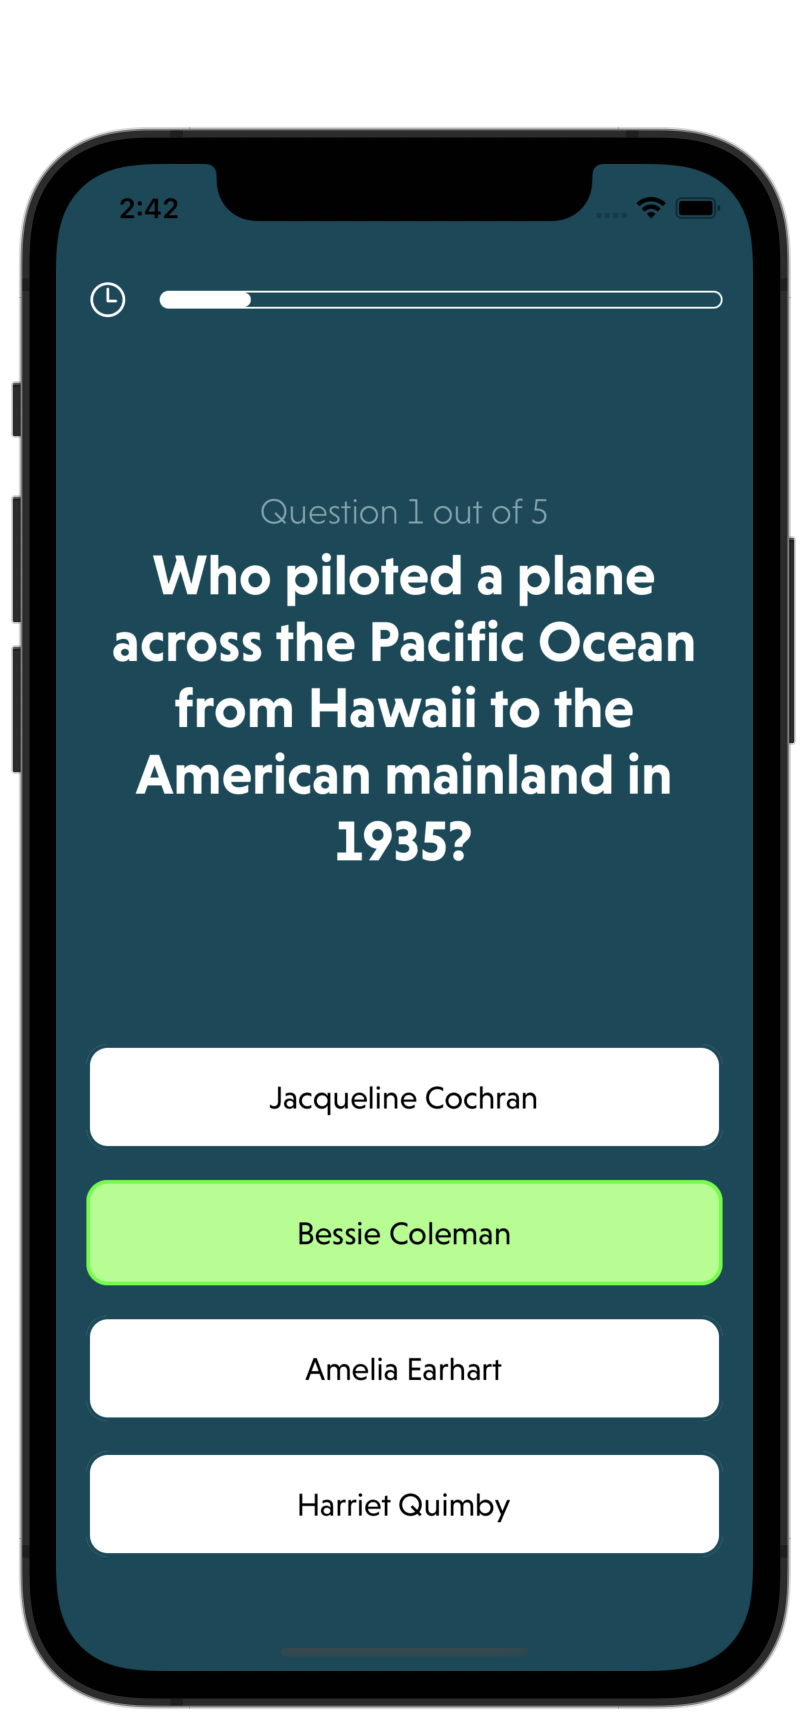
\includegraphics[width=\linewidth]{Mobile UI/User Selecting an option after starting a quiz.png}
        \caption{User selecting an option after starting a quiz}
    \end{minipage}
    \hspace{0.1\linewidth}
    \begin{minipage}[b]{0.43\linewidth}
        \centering
        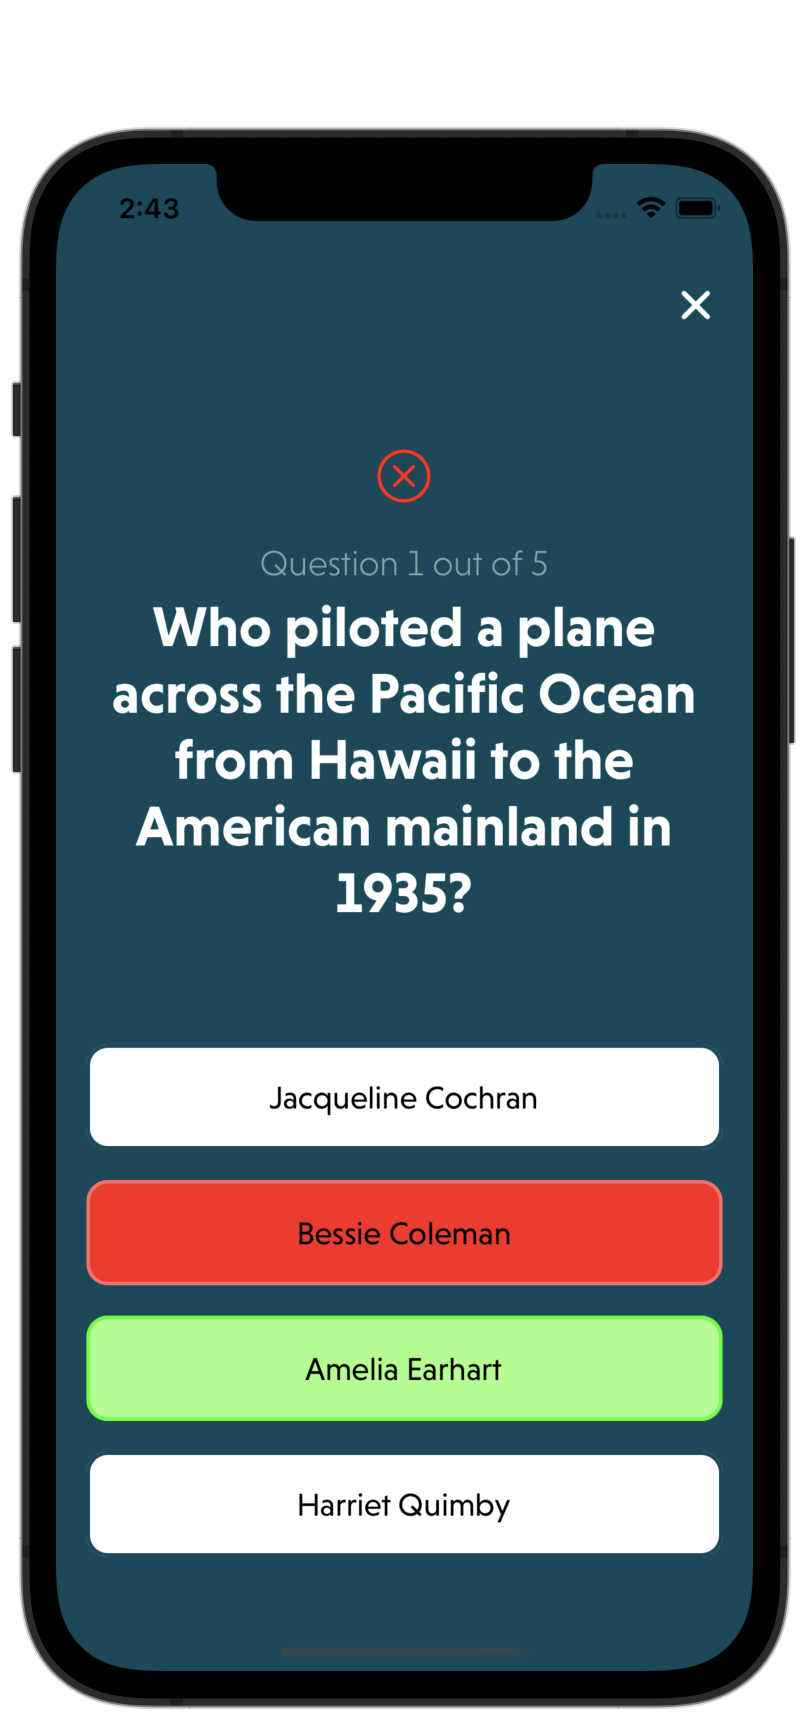
\includegraphics[width=\linewidth]{Mobile UI/Displaying correct result.png}
        \caption{Showing the result after the time has ended}
    \end{minipage}
    \vspace{0.5cm}
    \caption{\textbf{Starting a quiz and selecting an option}}
\end{figure}

\begin{itemize}
    \item The user begins the quiz by selecting a category and difficulty level.
    \item Each question is displayed one at a time, with multiple answer options provided below the question.
    \item When the user selects an option, it is highlighted to indicate their choice (Figure 23).
    \item Once the user submits their answer or the timer runs out, the correct answer is displayed:
    \begin{itemize}
        \item Correct answers are highlighted in green.
        \item Incorrect answers are highlighted in red (Figure 24).
        \item If the user did not select an answer, a message indicating "Did not select" is displayed, and then the correct answer is shown.
    \end{itemize}
    \item This immediate feedback helps users understand their mistakes and learn the correct information right away.
\end{itemize}

\vspace{1cm}

\subsubsection{Ending and Reviewing Quiz}

The ending and reviewing quiz screens provide users with a summary of their performance and an option to review their answers. These screens are designed to help users understand their mistakes and learn from them, enhancing the overall learning experience.

\begin{itemize}
    \item After completing a quiz, the user is presented with the quiz results screen.
    \item The quiz results screen displays the total number of questions, correct answers, and wrong answers.
    \item The user has the option to review their answers by tapping the "Review Answers" button.
    \item If the user chooses to review their answers:
    \begin{itemize}
        \item The quiz review screen displays each question along with the user's selected answer and the correct answer.
        \item Correct answers are highlighted in green icon, while incorrect answers are highlighted in red icon.
    \end{itemize}
    \item The user can also choose to return to the home page by tapping the "Return Home" button.
\end{itemize}

\begin{figure}[H]
    \centering
    \begin{minipage}[b]{0.43\linewidth}
        \centering
        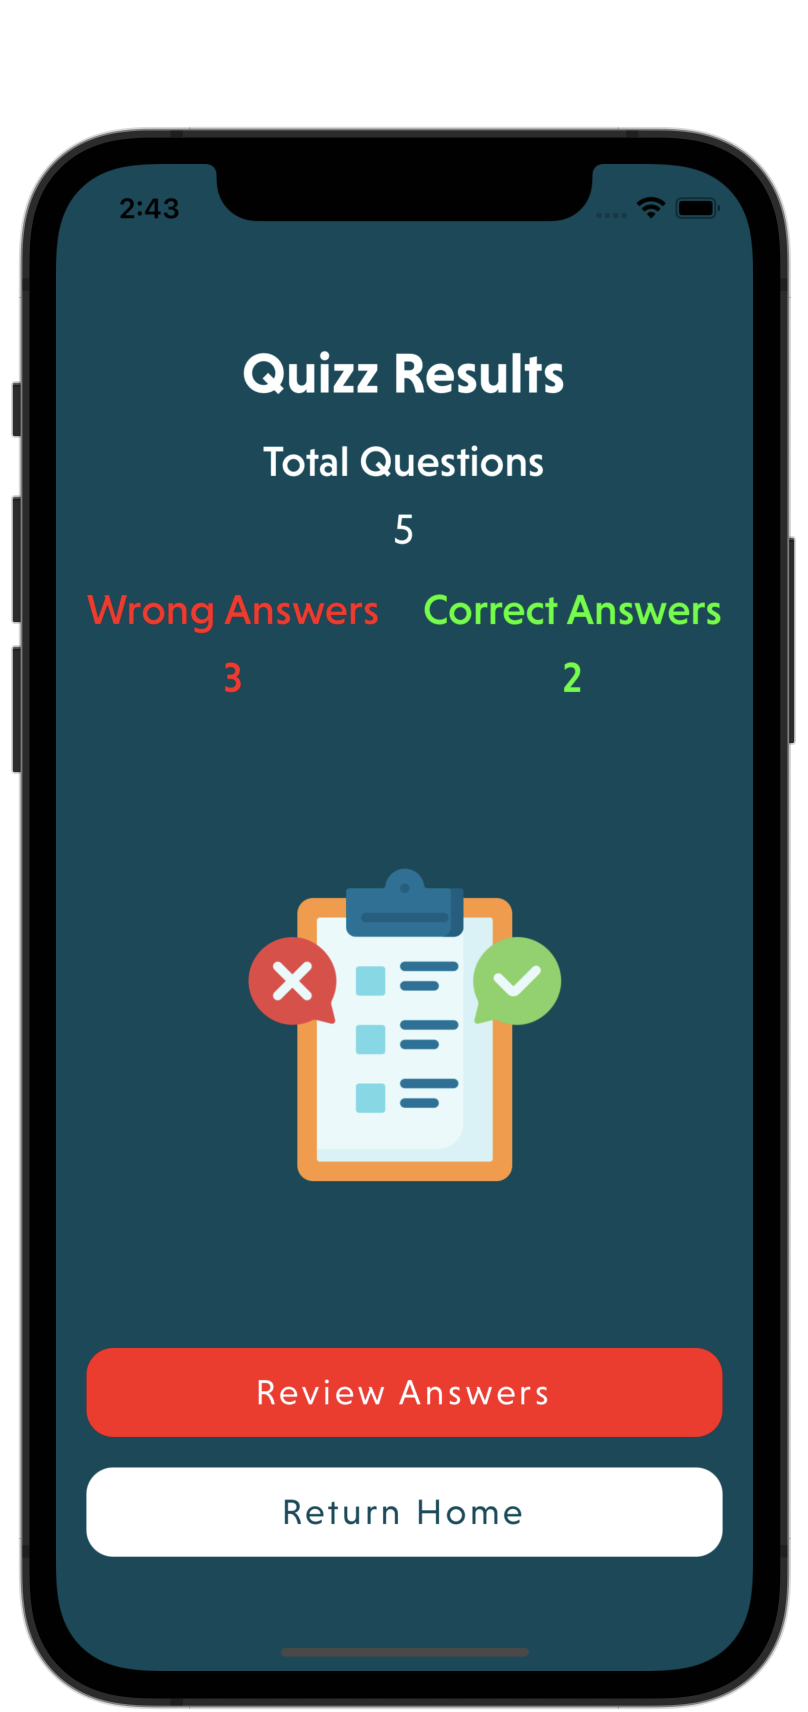
\includegraphics[width=\linewidth]{Mobile UI/Quiz Result.png}
        \caption{Quiz Results with options to review or return home}
    \end{minipage}
    \hspace{0.1\linewidth}
    \begin{minipage}[b]{0.43\linewidth}
        \centering
        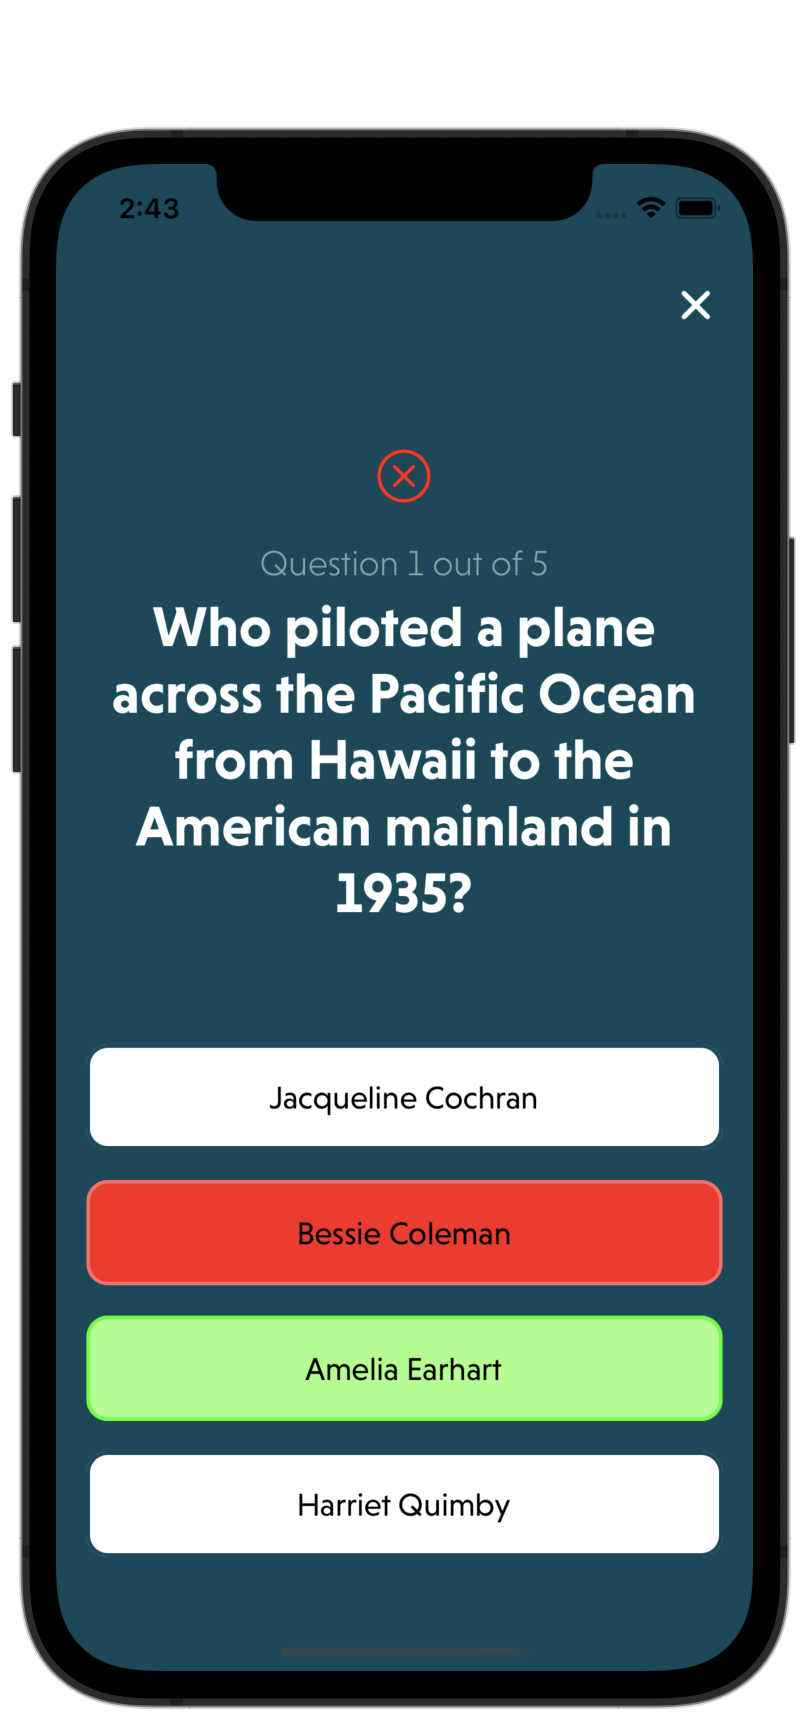
\includegraphics[width=\linewidth]{Mobile UI/Displaying correct result.png}
        \caption{Displaying correct result for incorrect solution}
    \end{minipage}
    \vspace{0.5cm}
    \caption{\textbf{Ending a quiz and selecting an option}}
\end{figure}


\begin{figure}[H]
    \centering
    \begin{minipage}[b]{0.43\linewidth}
        \centering
        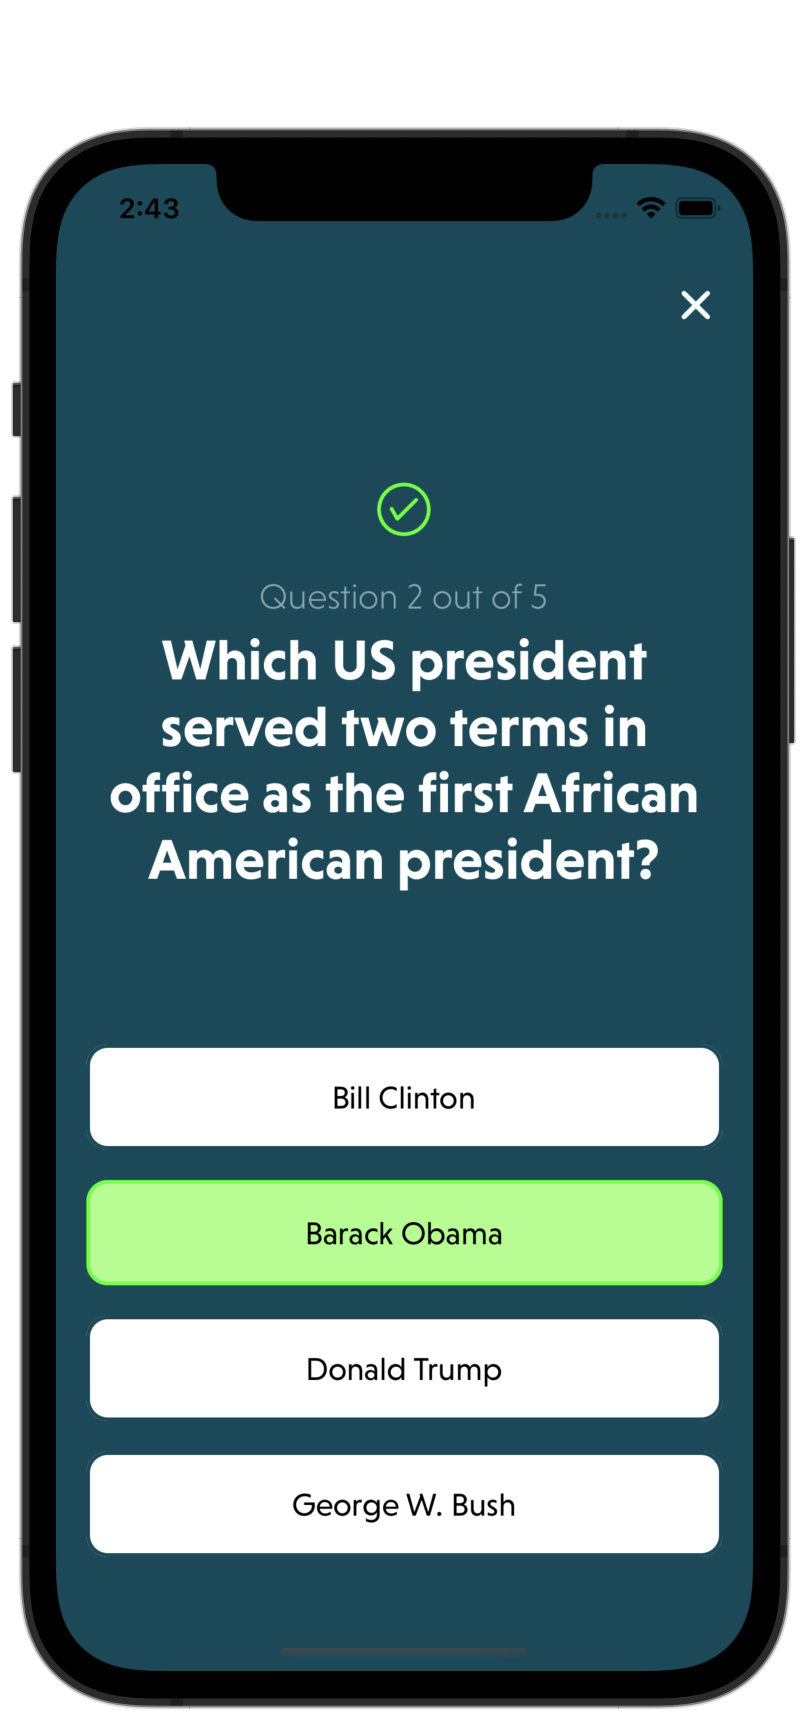
\includegraphics[width=\linewidth]{Mobile UI/Reviewing correct solution.png}
        \caption{Reviewing correct solution for correct selection}
    \end{minipage}
    \hspace{0.1\linewidth}
    \begin{minipage}[b]{0.43\linewidth}
        \centering
        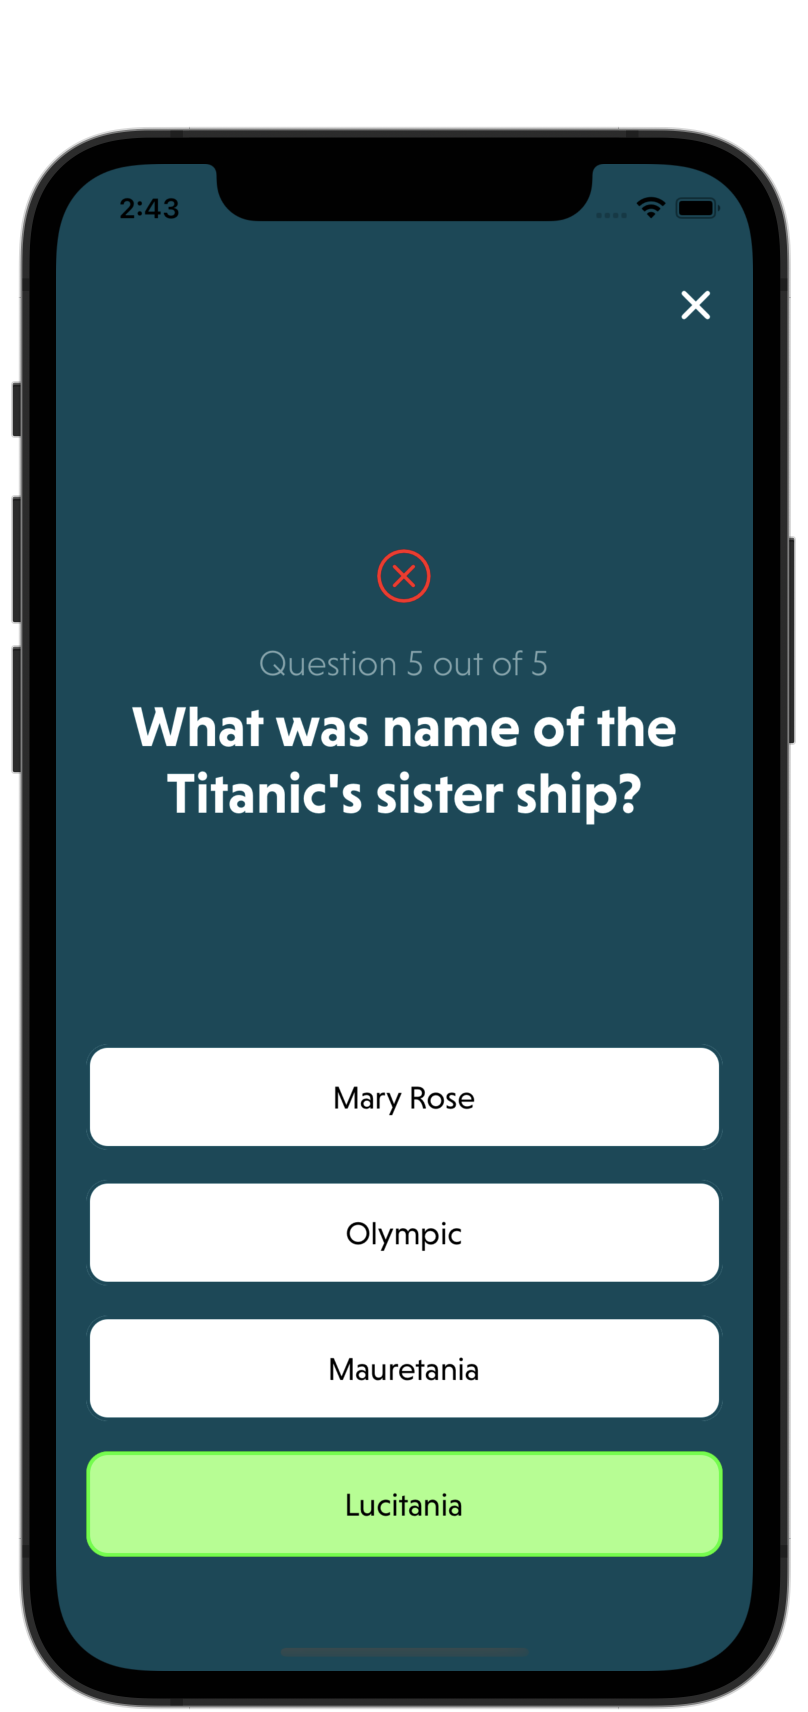
\includegraphics[width=\linewidth]{Mobile UI/Result when no selection has been made.png}
        \caption{Reviewing correct solution for no selection}
    \end{minipage}
    \vspace{0.5cm}
    \caption{\textbf{Reviewing the correct result}}
\end{figure}

\subsubsection{Leaderboard}

The leaderboard feature in the BrainMe application displays the ranking of users based on their quiz performance. This promotes a competitive environment, motivating users to improve their scores and climb the ranks. Users can view their position relative to others, fostering a sense of achievement and encouraging active participation in quizzes.

\begin{figure}[H]
    \centering
    \begin{minipage}[b]{0.3\linewidth}
        \centering
        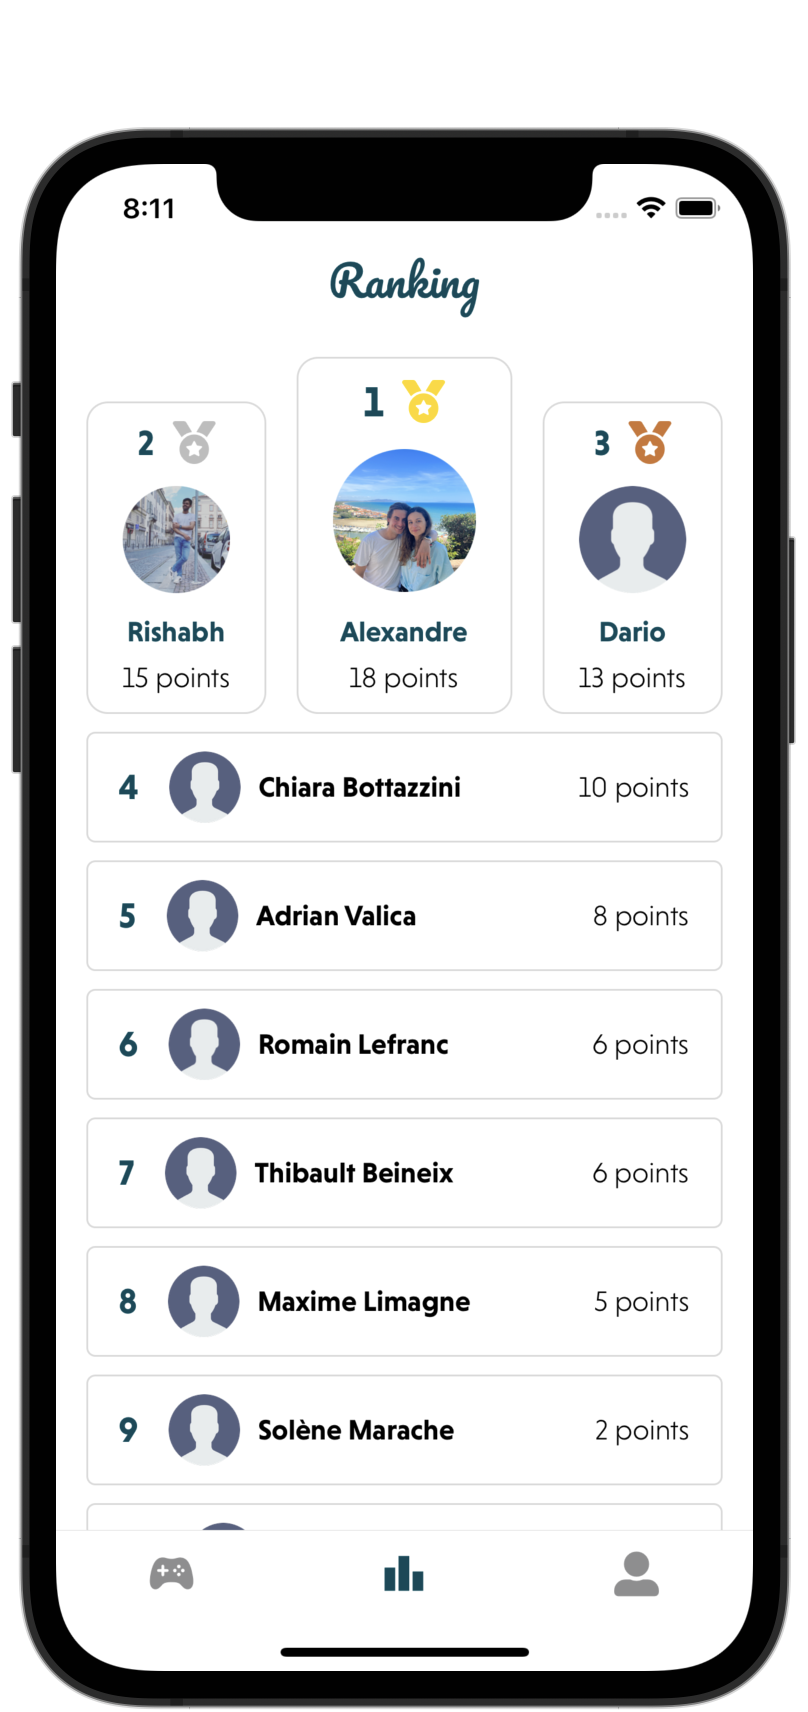
\includegraphics[width=\linewidth]{Mobile UI/Initial Leaderboard.png}
        \caption{Leaderboard ranking depicting medals and rankings}
    \end{minipage}
    \hspace{0.02\linewidth}
    \begin{minipage}[b]{0.3\linewidth}
        \centering
        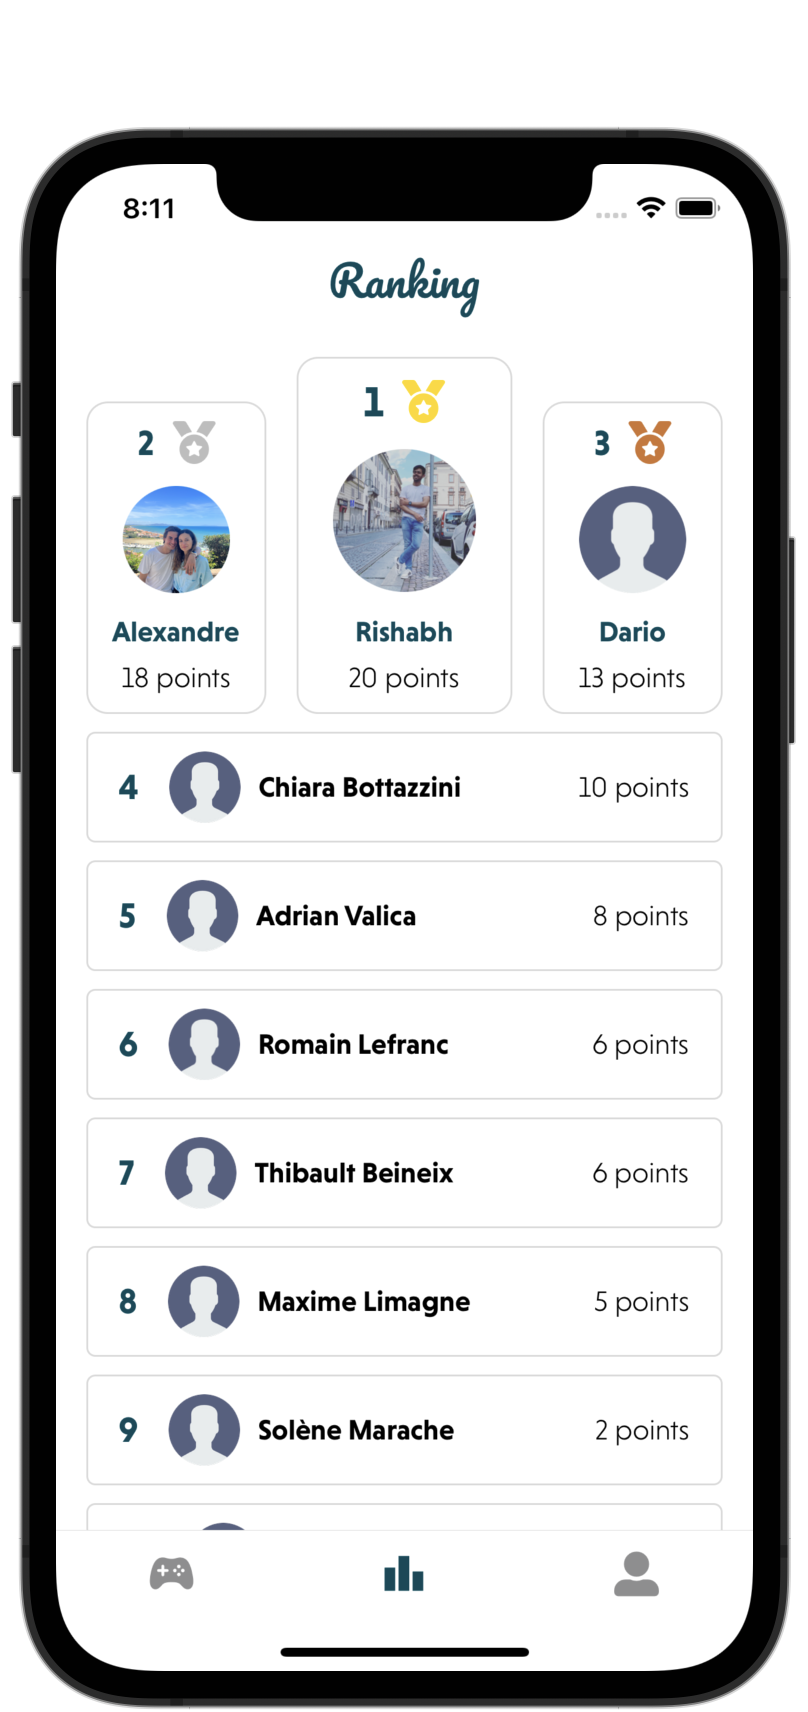
\includegraphics[width=\linewidth]{Mobile UI/Final Leaderboard.png}
        \caption{Change in leaderboard position from second to first}
    \end{minipage}
    \hspace{0.02\linewidth}
    \begin{minipage}[b]{0.3\linewidth}
        \centering
        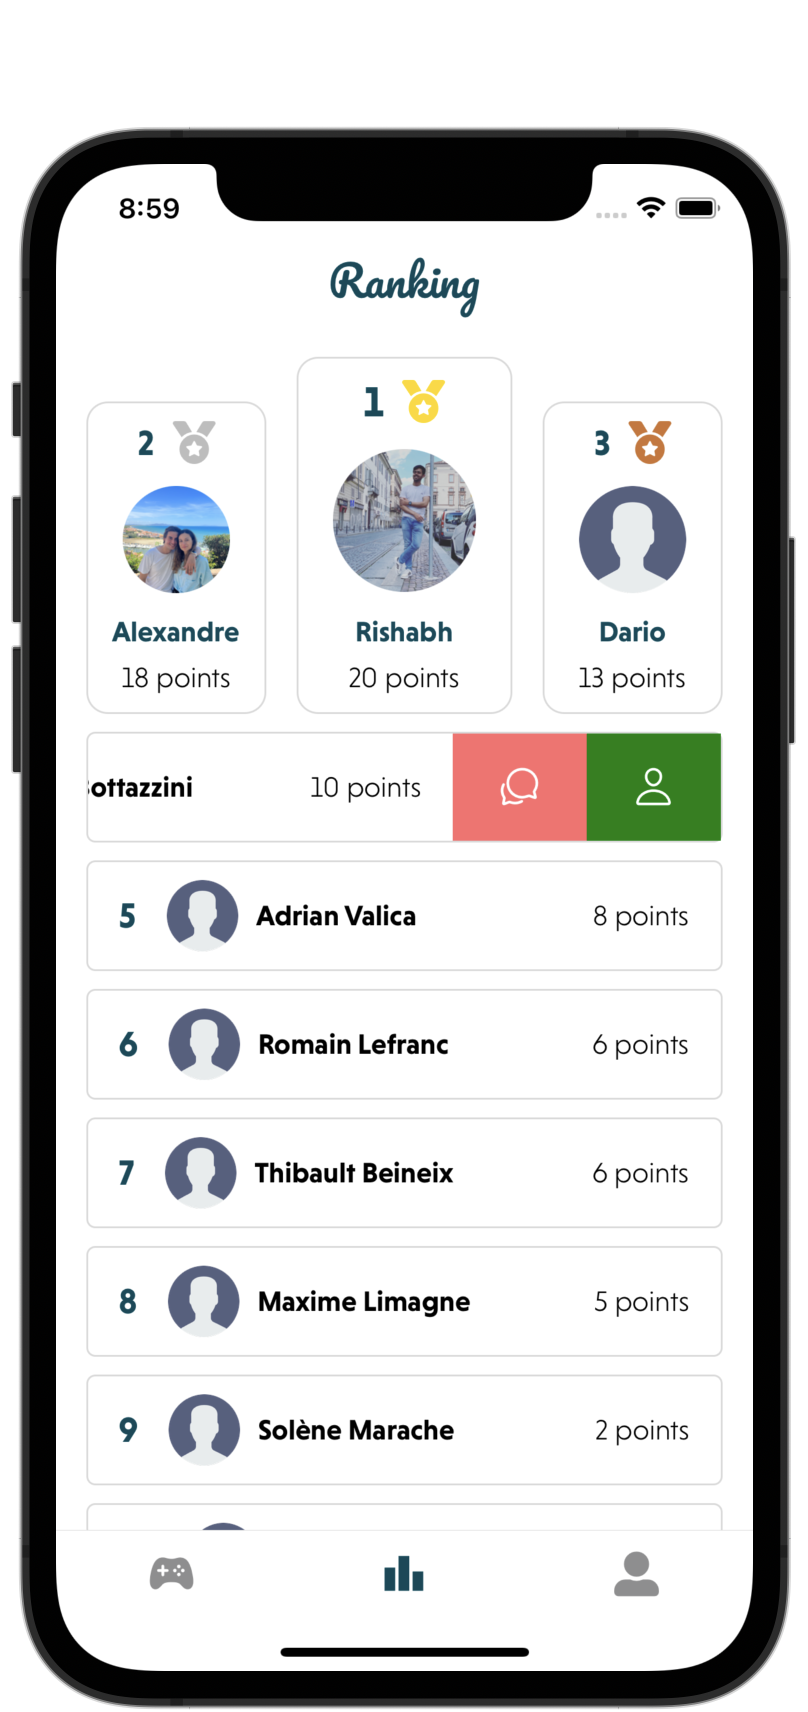
\includegraphics[width=\linewidth]{leaderboard chat.png}
        \caption{Sliding on the name to chat or view profile}
    \end{minipage}
    \vspace{0.5cm}
    \caption{\textbf{Depicting a change in the position of leaderboard ranking and the medals along with chat option}}
\end{figure}


\begin{itemize}
\item \textbf{Real-time updates:} The leaderboard is updated in real-time to reflect the latest user rankings based on quiz performance.
\item \textbf{Visual indicators:} Medals for the top three users provide immediate visual recognition of the leading participants.
\item \textbf{User details:} Displaying usernames and profile pictures makes the leaderboard more personal and engaging.
\item \textbf{Sliding feature} Allows registered users to send message or view their profile directly from the leaderboard rankings.
\item \textbf{Motivation and engagement:} The competitive nature of the leaderboard encourages users to participate more actively in quizzes to improve their ranking.
\end{itemize}

\subsubsection{Profile Page}

\begin{figure}[H]
    \centering
    \begin{minipage}[b]{0.43\linewidth}
        \centering
        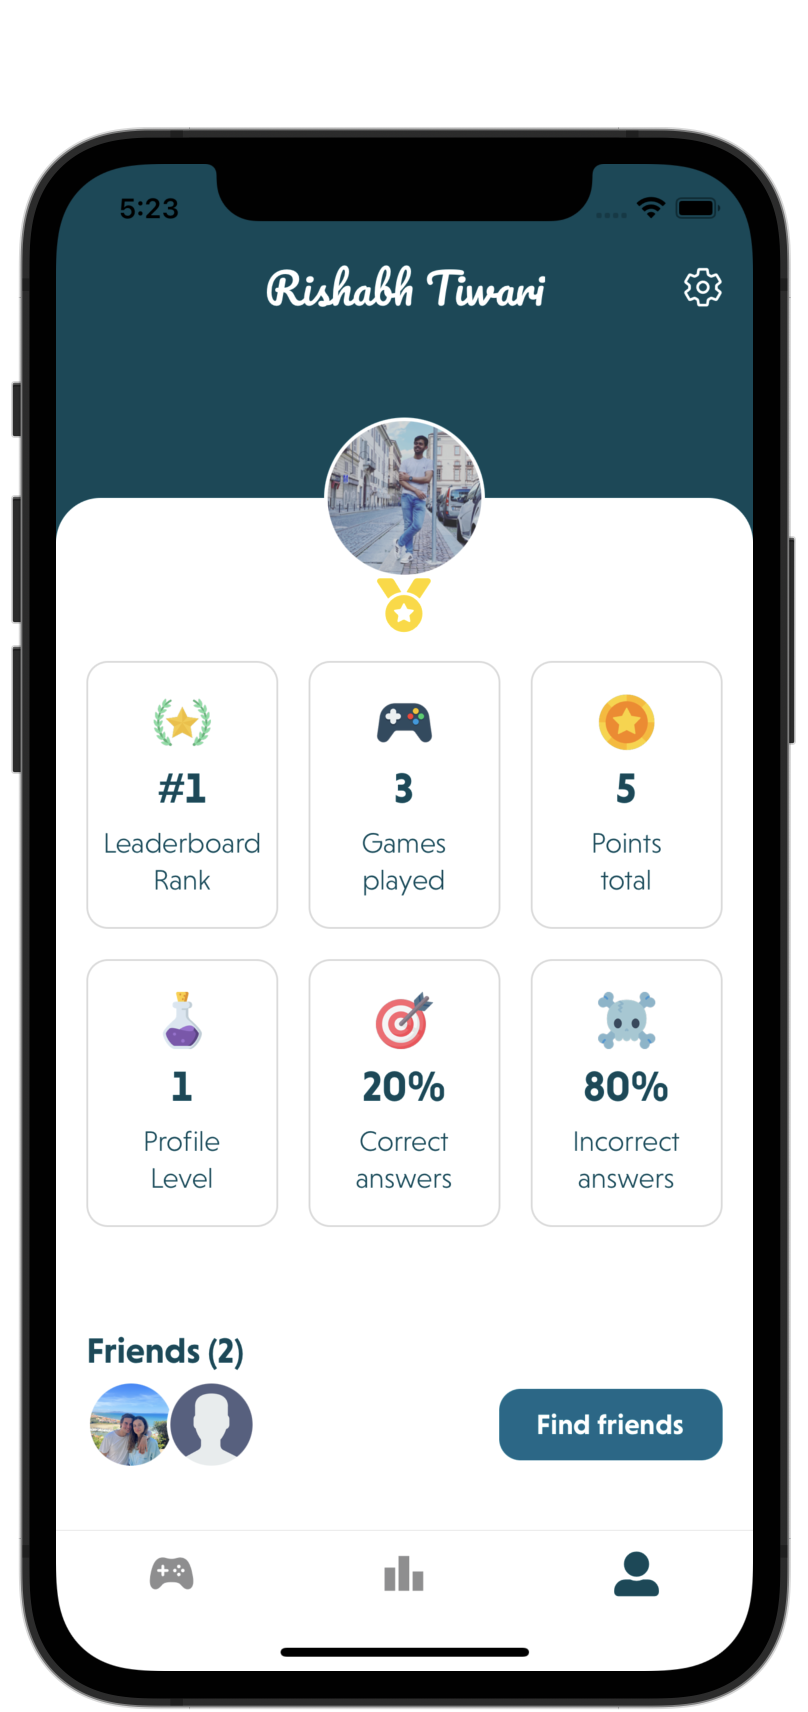
\includegraphics[width=\linewidth]{Screens_UI/My Profile.png}
        \caption{\textbf{User Profile UI with Statistics}}
    \end{minipage}
\end{figure}


The Profile Page offers a comprehensive overview of the user's achievements and statistics within the BrainMe application. At the top, users can see their profile picture and username, providing a personalized touch. Below this, various statistics and achievements are displayed, including:

\begin{itemize}
\item \textbf{Leaderboard Rank:} Shows the user's current rank on the leaderboard, motivating them to improve their performance.
\item \textbf{Games Played:} Displays the total number of games the user has participated in.
\item \textbf{Points Total:} Indicates the total points accumulated by the user.
\item \textbf{Profile Level:} Represents the user's profile level based on their activity and achievements.
\item \textbf{Correct Answers:} Shows the percentage of questions the user has answered correctly.
\item \textbf{Incorrect Answers:} Displays the percentage of questions the user has answered incorrectly.
\end{itemize}

Additionally, there is a "Find Friends" button that allows users to search for and connect with other users within the app, enhancing the social learning experience. The clean and intuitive design ensures that users can easily access and understand their statistics, fostering a sense of achievement and encouraging continuous engagement with the app.

\subsubsection{Friend list and checking other user's profile}

The Friend List and Checking Other User's Profile feature in BrainMe enhances the social interaction aspect of the application. It allows users to view the friends they already follow and view their progress and achievements.

\begin{itemize}
\item \textbf{Friend List:} The left screen (Figure 33) displays the user's friends list. Users can see their friends' names, profile pictures, and the points they have earned. A search bar at the top allows users to quickly find specific friends by name.
\item \textbf{Friend's User Profile:} The right screen (Figure 34) shows a friend's detailed profile when selected from the friends list. The profile includes the friend's leaderboard rank, games played, total points, profile level, correct answer percentage, and incorrect answer percentage. Additionally, users can send a message or unfollow the friend using the buttons provided.
\end{itemize}

This feature promotes a competitive and collaborative environment, motivating users to improve their performance by comparing their achievements with those of their friends.



\begin{figure}[H]
    \centering
    \begin{minipage}[b]{0.43\linewidth}
        \centering
        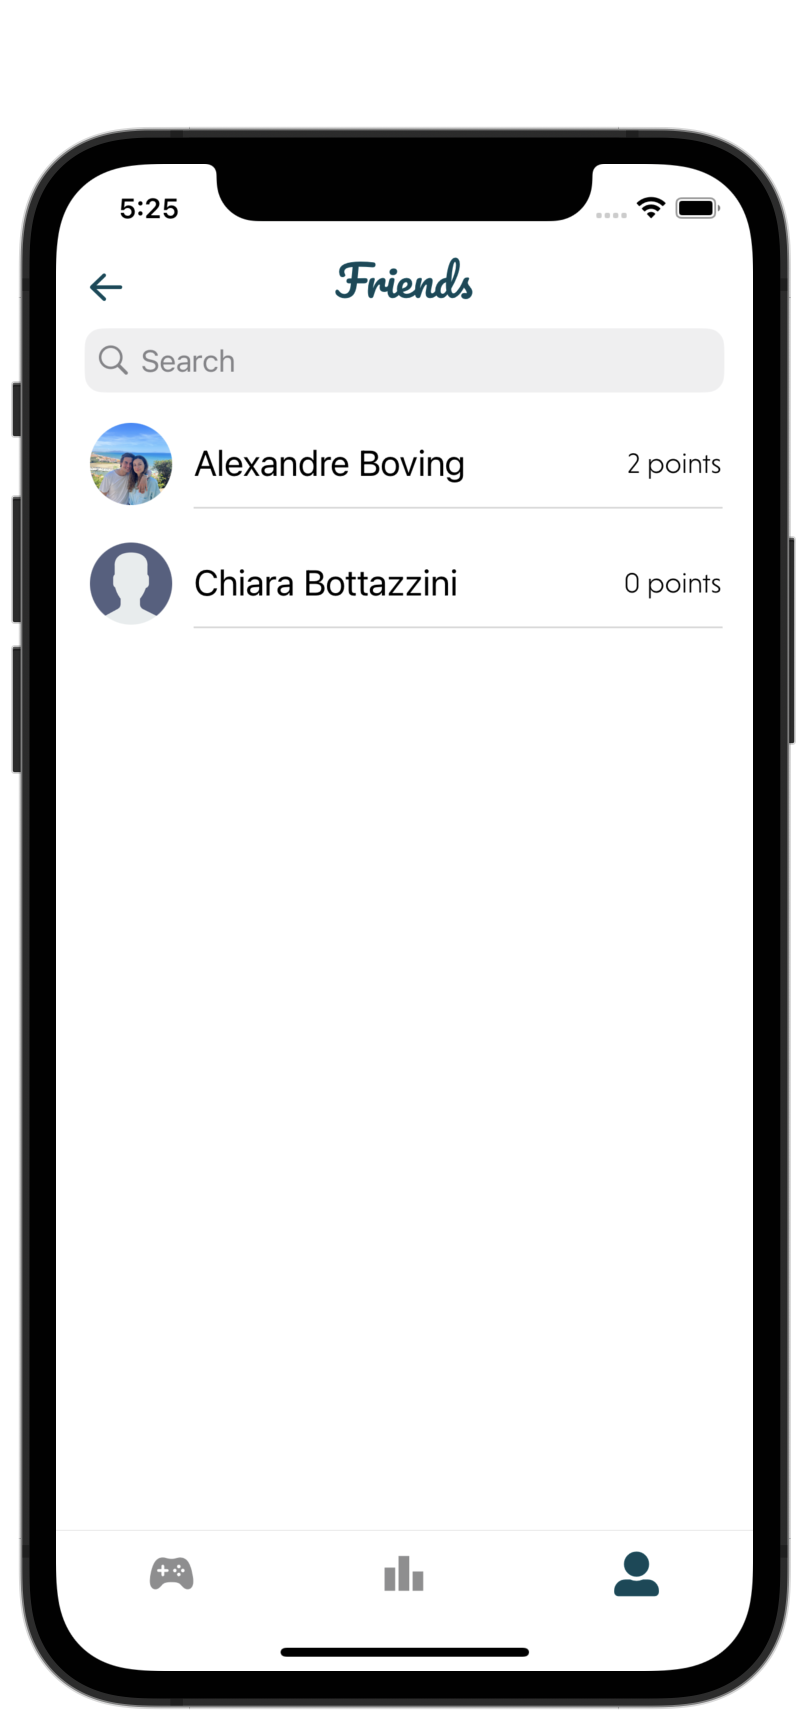
\includegraphics[width=\linewidth]{Mobile UI/Friend List.png}
        \caption{User's friends list}
    \end{minipage}
    \hspace{0.1\linewidth}
    \begin{minipage}[b]{0.43\linewidth}
        \centering
        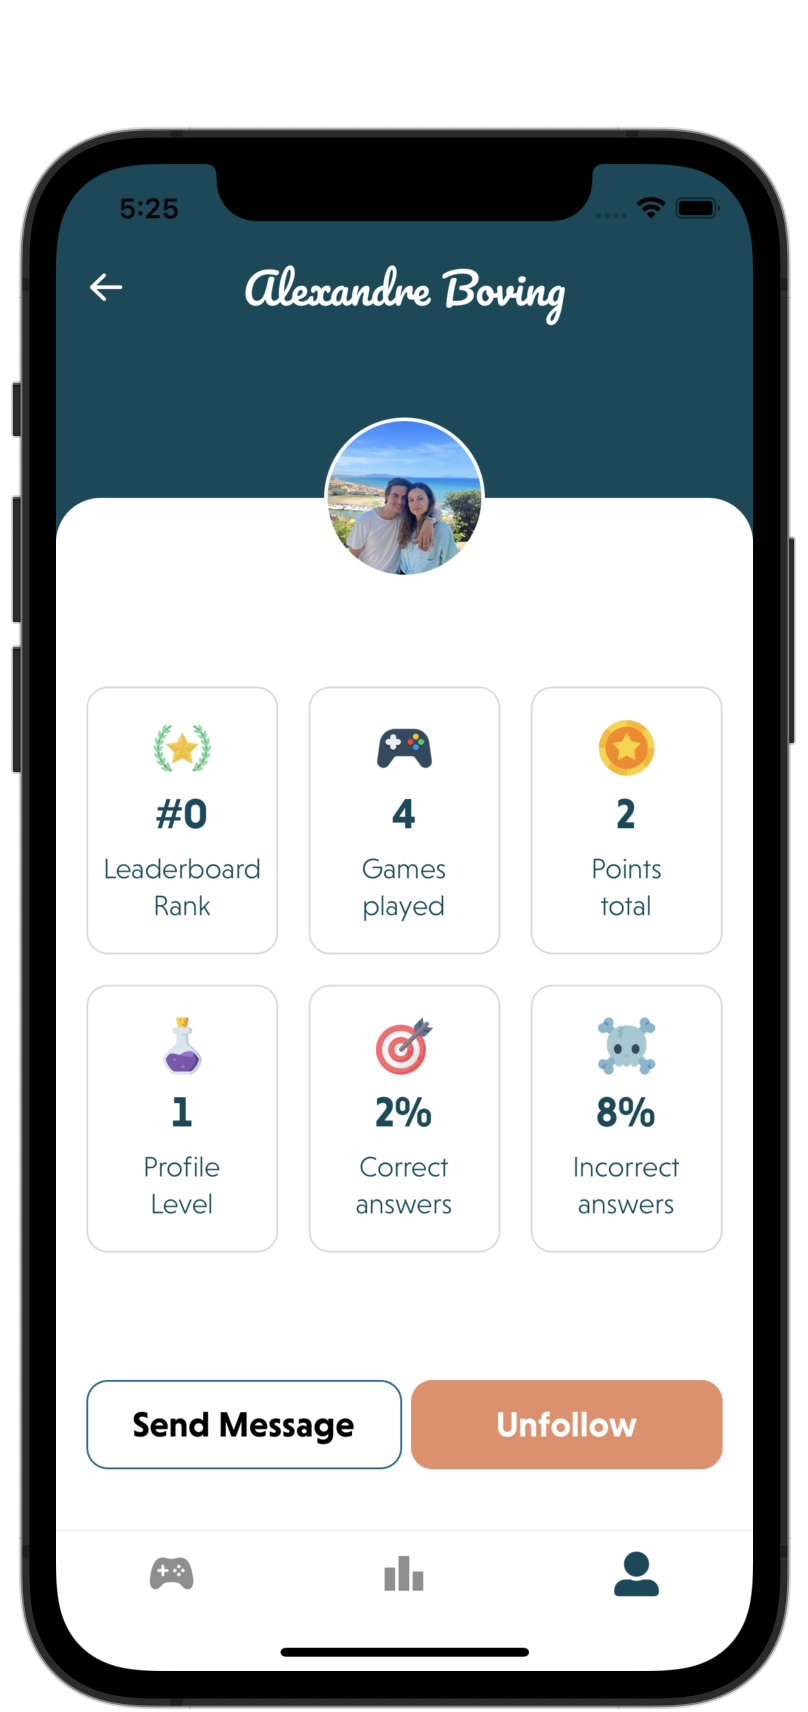
\includegraphics[width=\linewidth]{Mobile UI/Friend's Profile.png}
        \caption{Friend's User Profile}
    \end{minipage}
    \vspace{0.5cm}
    \caption{\textbf{User's friend list along with friend's user profile}}
\end{figure}

\subsubsection{Find Friends}

\begin{figure}[H]
    \centering
    \begin{minipage}[b]{0.43\linewidth}
        \centering
        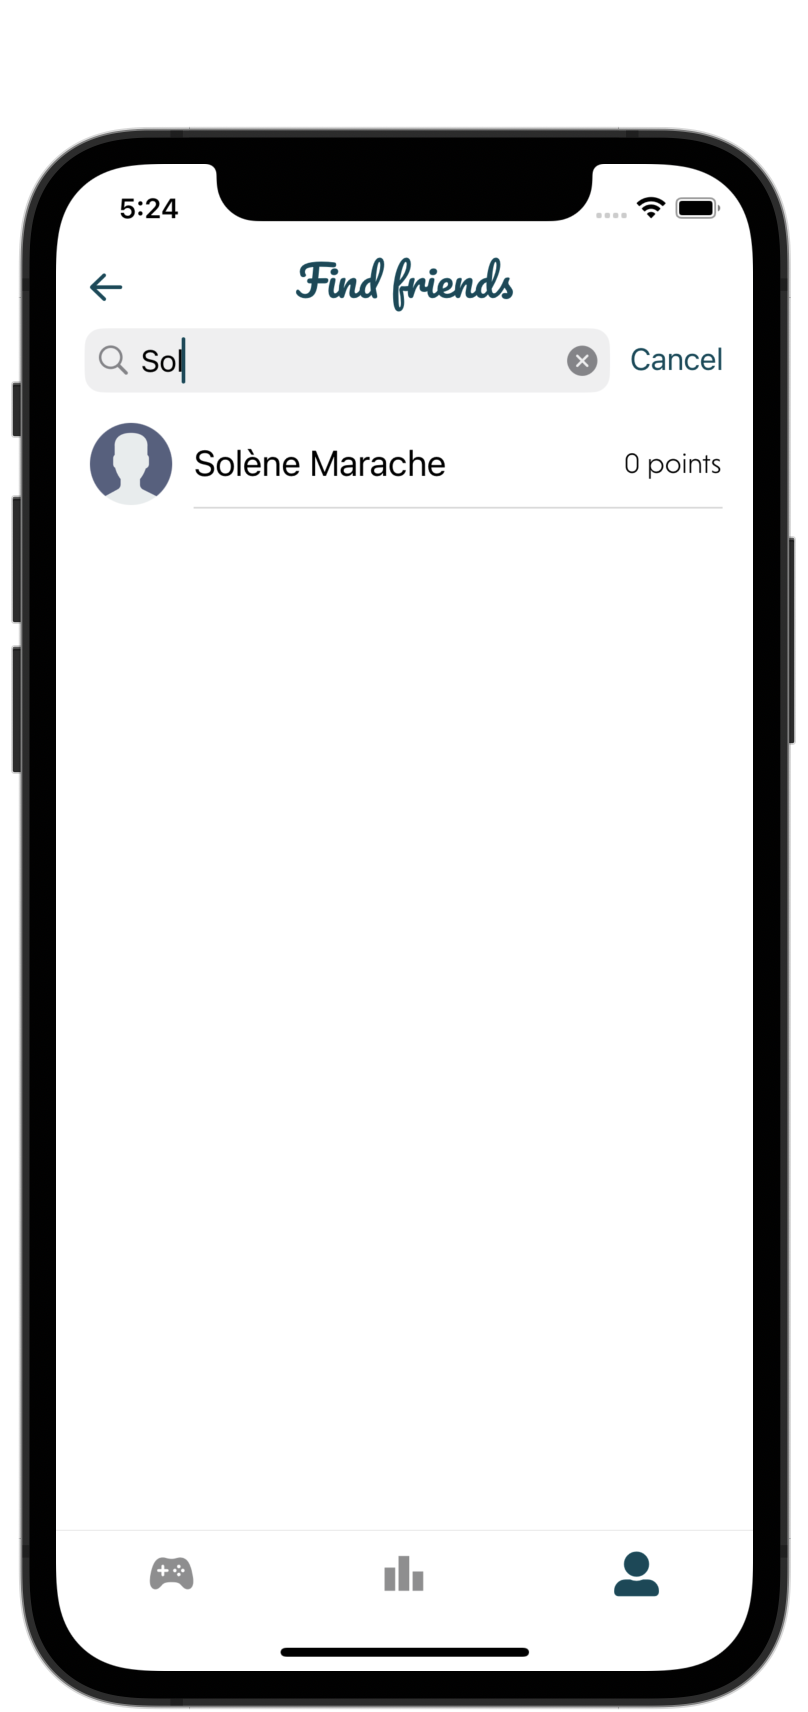
\includegraphics[width=\linewidth]{Mobile UI/Find Friends.png}
        \caption{Searching for a friend from the available users}
    \end{minipage}
    \hspace{0.1\linewidth}
    \begin{minipage}[b]{0.43\linewidth}
        \centering
        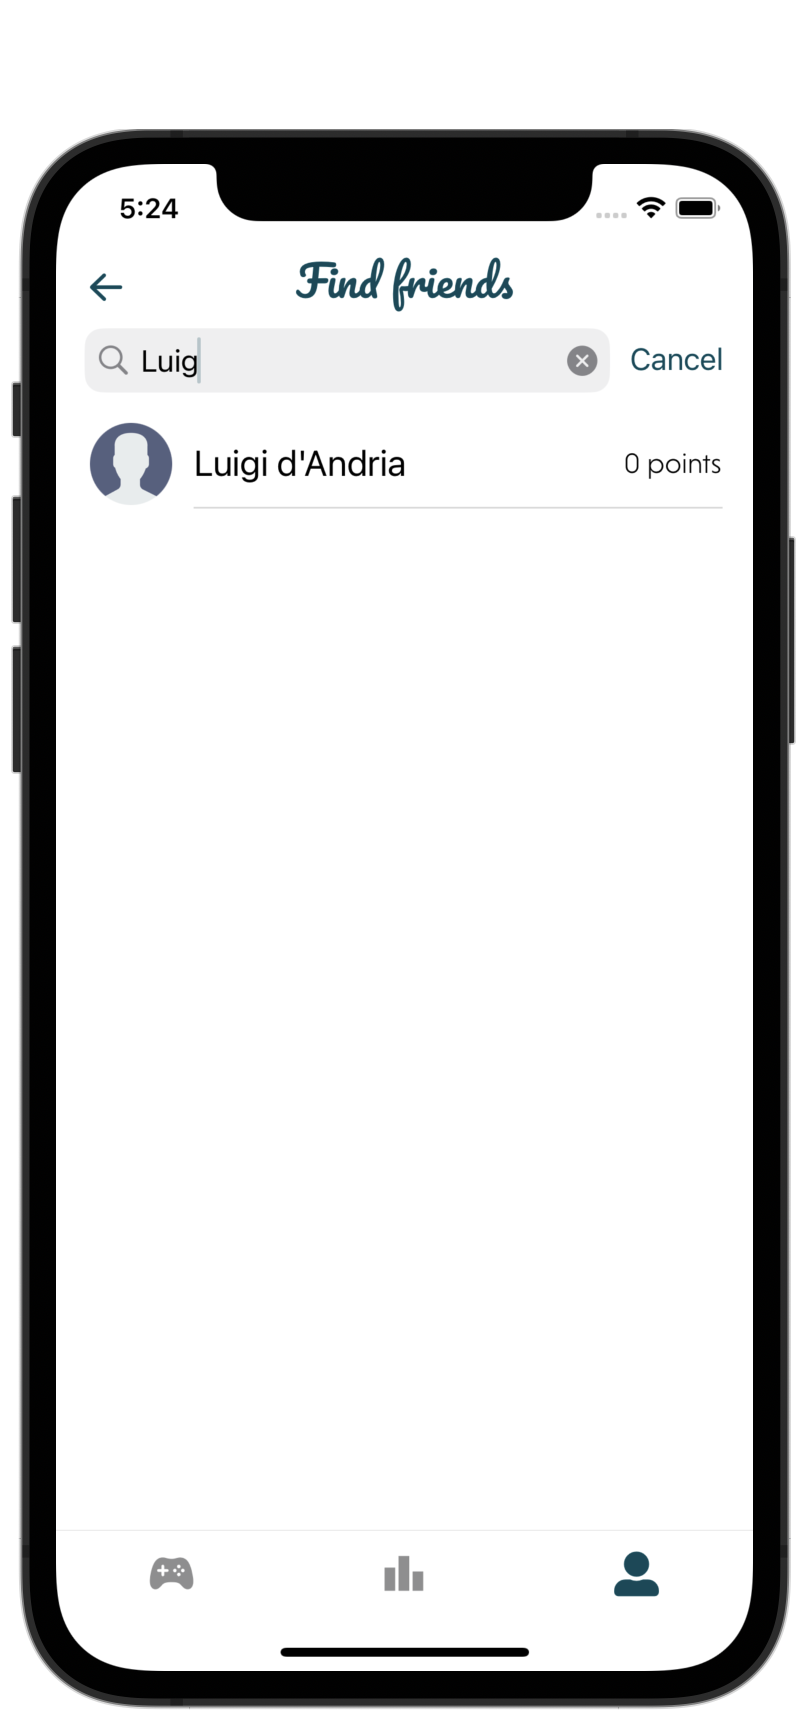
\includegraphics[width=\linewidth]{Mobile UI/Find Friends 1.png}
        \caption{Filter search for following a friend}
    \end{minipage}
    \vspace{0.5cm}
    \caption{\textbf{User can search for a friend and follow them}}
\end{figure}

The Find Friends feature in BrainMe allows users to search for and connect with other users. This promotes social interaction and collaboration within the application.

\begin{itemize}
\item \textbf{Searching for a Friend:} The left screen (Figure 36) shows the user entering a friend's name into the search bar. As the user types, the app filters the list to display matching names. This makes it easy for users to find specific friends quickly.
\item \textbf{Filter Search for Adding:} The right screen (Figure 37) displays the results of the search, showing the user’s profile picture, name, and points. Users can select a friend from the list to view their profile and follow them.
\end{itemize}

\subsubsection{Chat Page}

\begin{figure}[H]
    \centering
    \begin{minipage}[b]{0.43\linewidth}
        \centering
        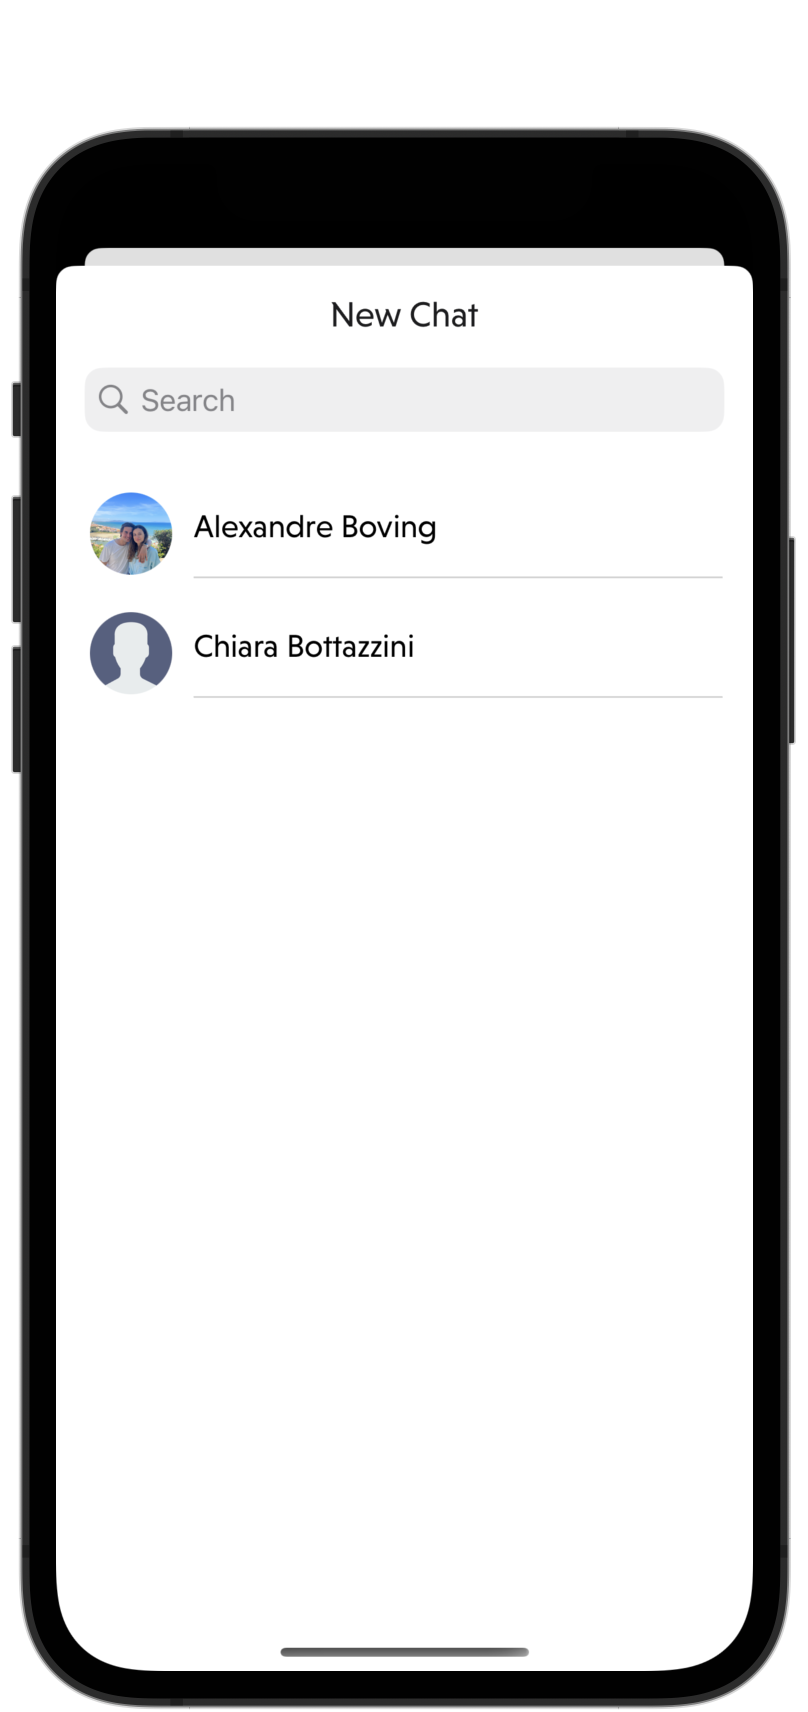
\includegraphics[width=\linewidth]{Images/New Chat Selection.png}
        \caption{Creating new chat}
    \end{minipage}
    \hspace{0.1\linewidth}
    \begin{minipage}[b]{0.43\linewidth}
        \centering
        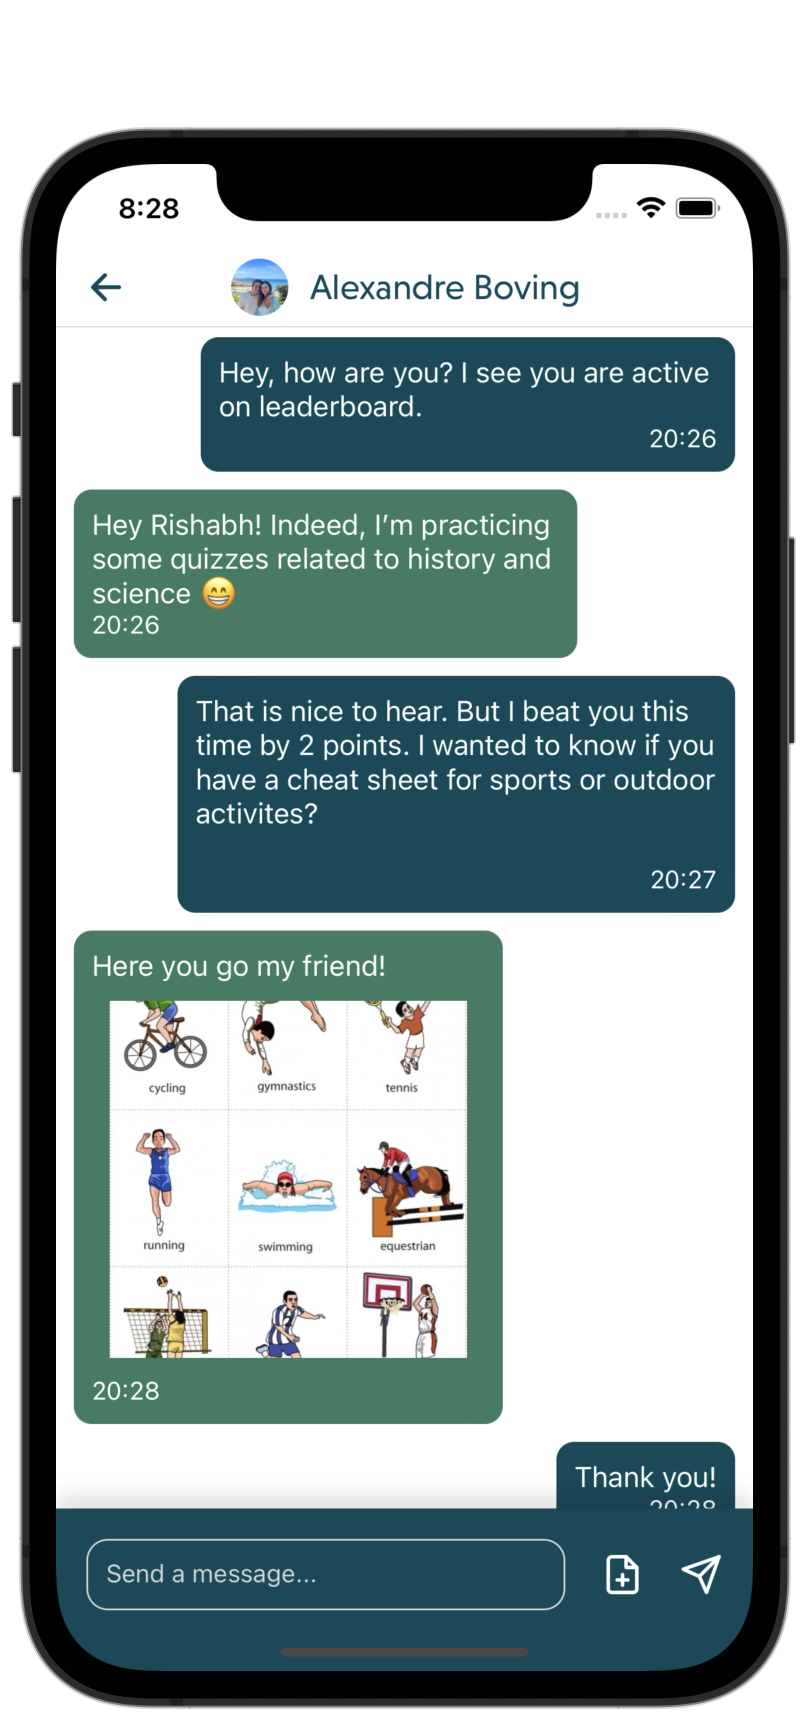
\includegraphics[width=\linewidth]{Images/Chat Example.png}
        \caption{Chat System Example}
    \end{minipage}
    \vspace{0.5cm}
    \caption{\textbf{Creation and an example of a new chat with file sharing}}
\end{figure}

The chat page allows users to create new chats and engage in conversations with other users. This feature supports both text and file sharing, enhancing the communication experience within the app.

\begin{itemize}
    \item \textbf{Creating New Chat:} Users can easily initiate a new chat with their friends by selecting from a list of contacts.
    \item \textbf{Chat System Example:} The chat interface displays messages exchanged between users, including the time stamps and any shared files.
    \item \textbf{File Sharing:} Users can share images and other files within the chat, making it more interactive and engaging.
\end{itemize}

\vspace{1cm}

\subsubsection{Settings Page}

The Settings Page in BrainMe provides users with the ability to manage their account details and preferences, ensuring a personalized and secure experience.

\begin{itemize}
\item \textbf{Account Settings Page:} The left screen (Figure 39) shows the account settings page where users can view and update their personal information, such as their name and family name. This screen also includes options for managing push notifications and account security, like signing out or deleting the account.
\item \textbf{Push Notifications:} The right screen (Figure 40) displays the toggle switch for push notifications. Users can easily turn notifications on or off according to their preference, ensuring they stay informed about important updates without being overwhelmed.
\end{itemize}

\begin{figure}[H]
    \centering
    \begin{minipage}[b]{0.43\linewidth}
        \centering
        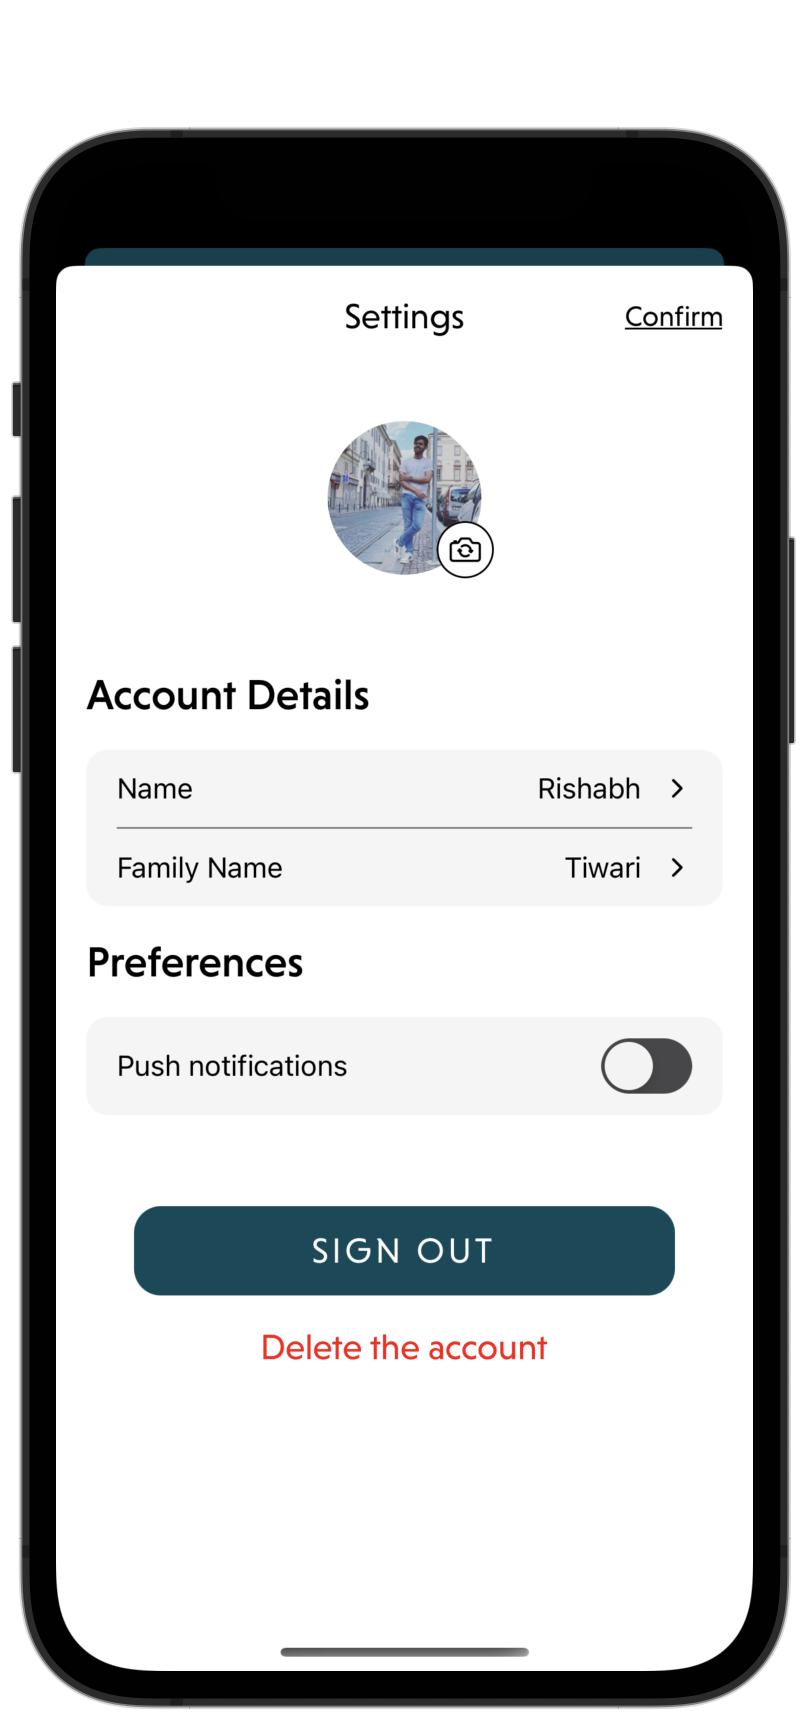
\includegraphics[width=\linewidth]{Mobile UI/Account Settings.png}
        \caption{Account Settings Page}
    \end{minipage}
    \hspace{0.1\linewidth}
    \begin{minipage}[b]{0.43\linewidth}
        \centering
        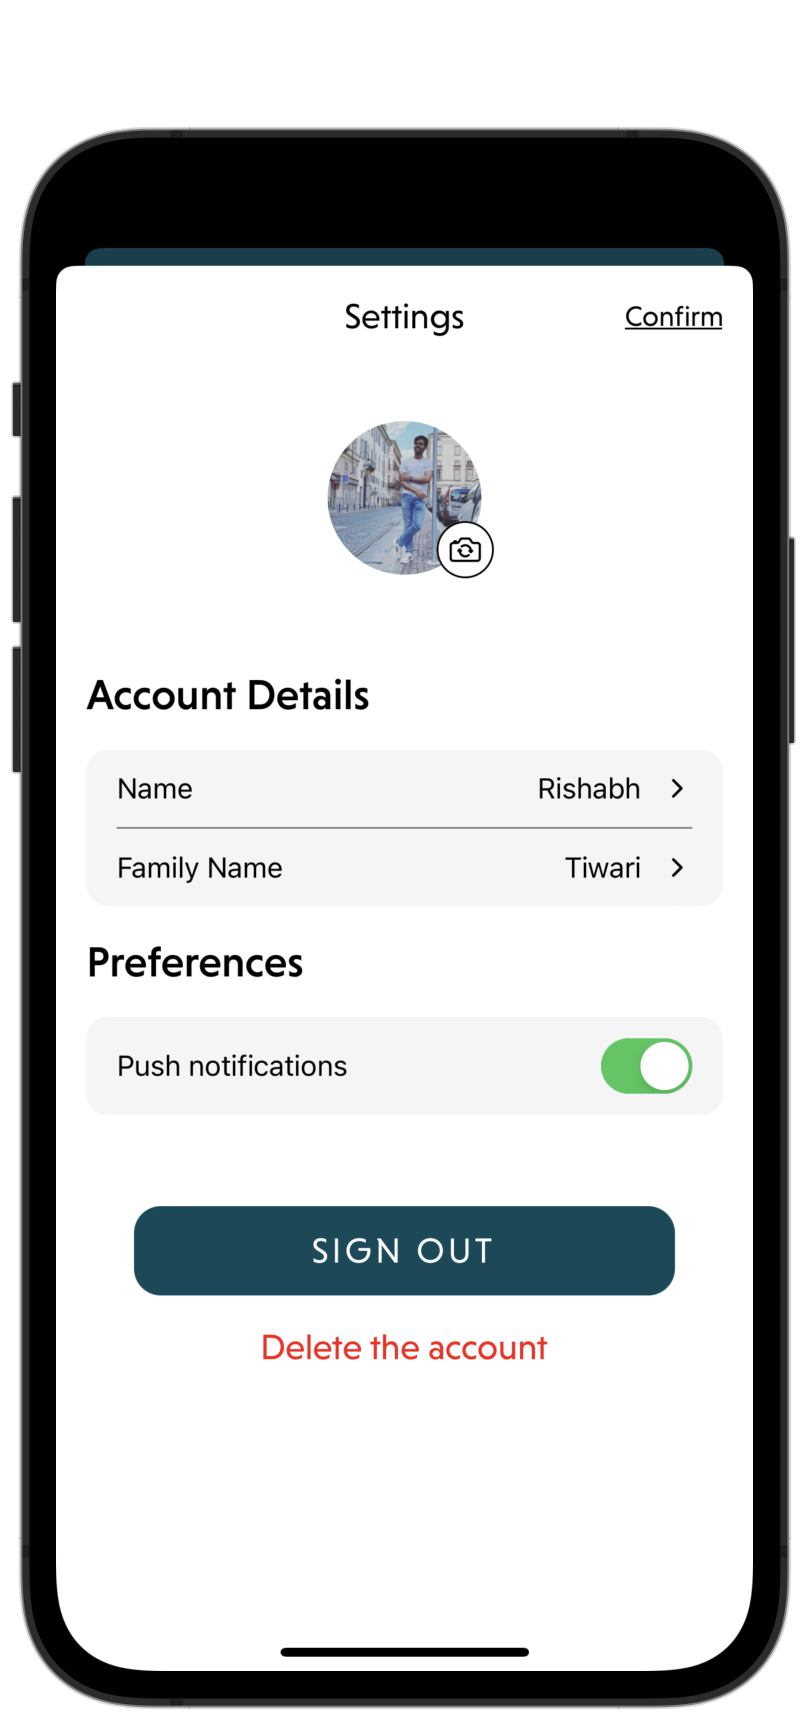
\includegraphics[width=\linewidth]{Mobile UI/Push Notifications.png}
        \caption{Push Notifications}
    \end{minipage}
    \vspace{0.5cm}
    \caption{\textbf{Account Settings with Push Notifications}}
\end{figure}



\subsection{Tablet UI}
\subsubsection{Login Page and SignUp Page}


\begin{figure}[H]
    \centering
    \begin{minipage}[b]{0.43\linewidth}
        \centering
        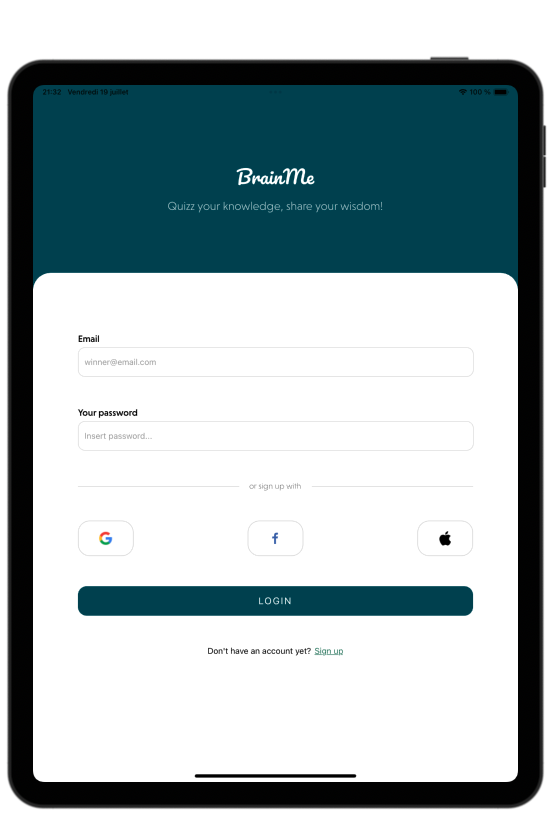
\includegraphics[height=10cm]{TabletUI/Login Page.png}
        \caption{Login Page}
    \end{minipage}
    \hspace{0.1\linewidth}
    \begin{minipage}[b]{0.43\linewidth}
        \centering
        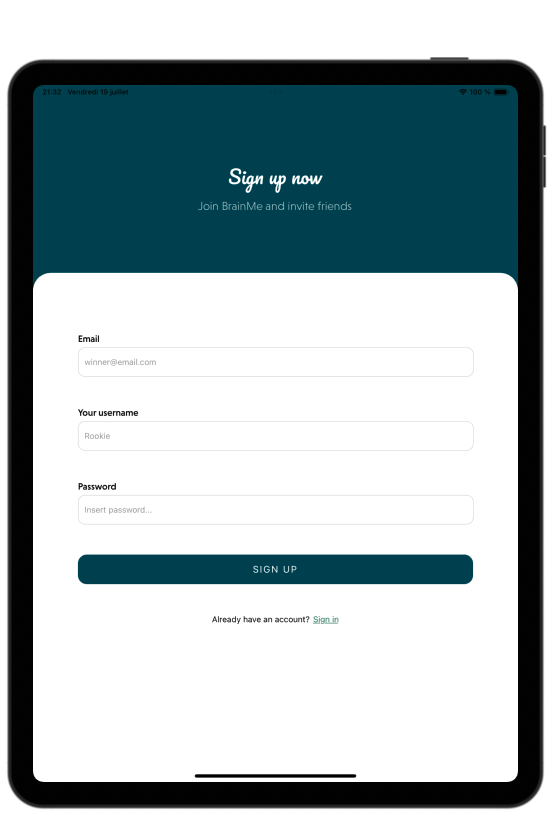
\includegraphics[height=10cm]{TabletUI/Sign Up Page.png}
        \caption{Sign Up Page}
    \end{minipage}
    \vspace{0.5cm}
    \caption{\textbf{The BrainMe Application}}
\end{figure}

The above screen performs the same functions as the Ipphone screens. The user can sign up and login using the respective email or single sign on methods.

\subsubsection{Quiz Page: }

\begin{figure}[H]
    \centering
    \begin{minipage}[b]{0.43\linewidth}
        \centering
        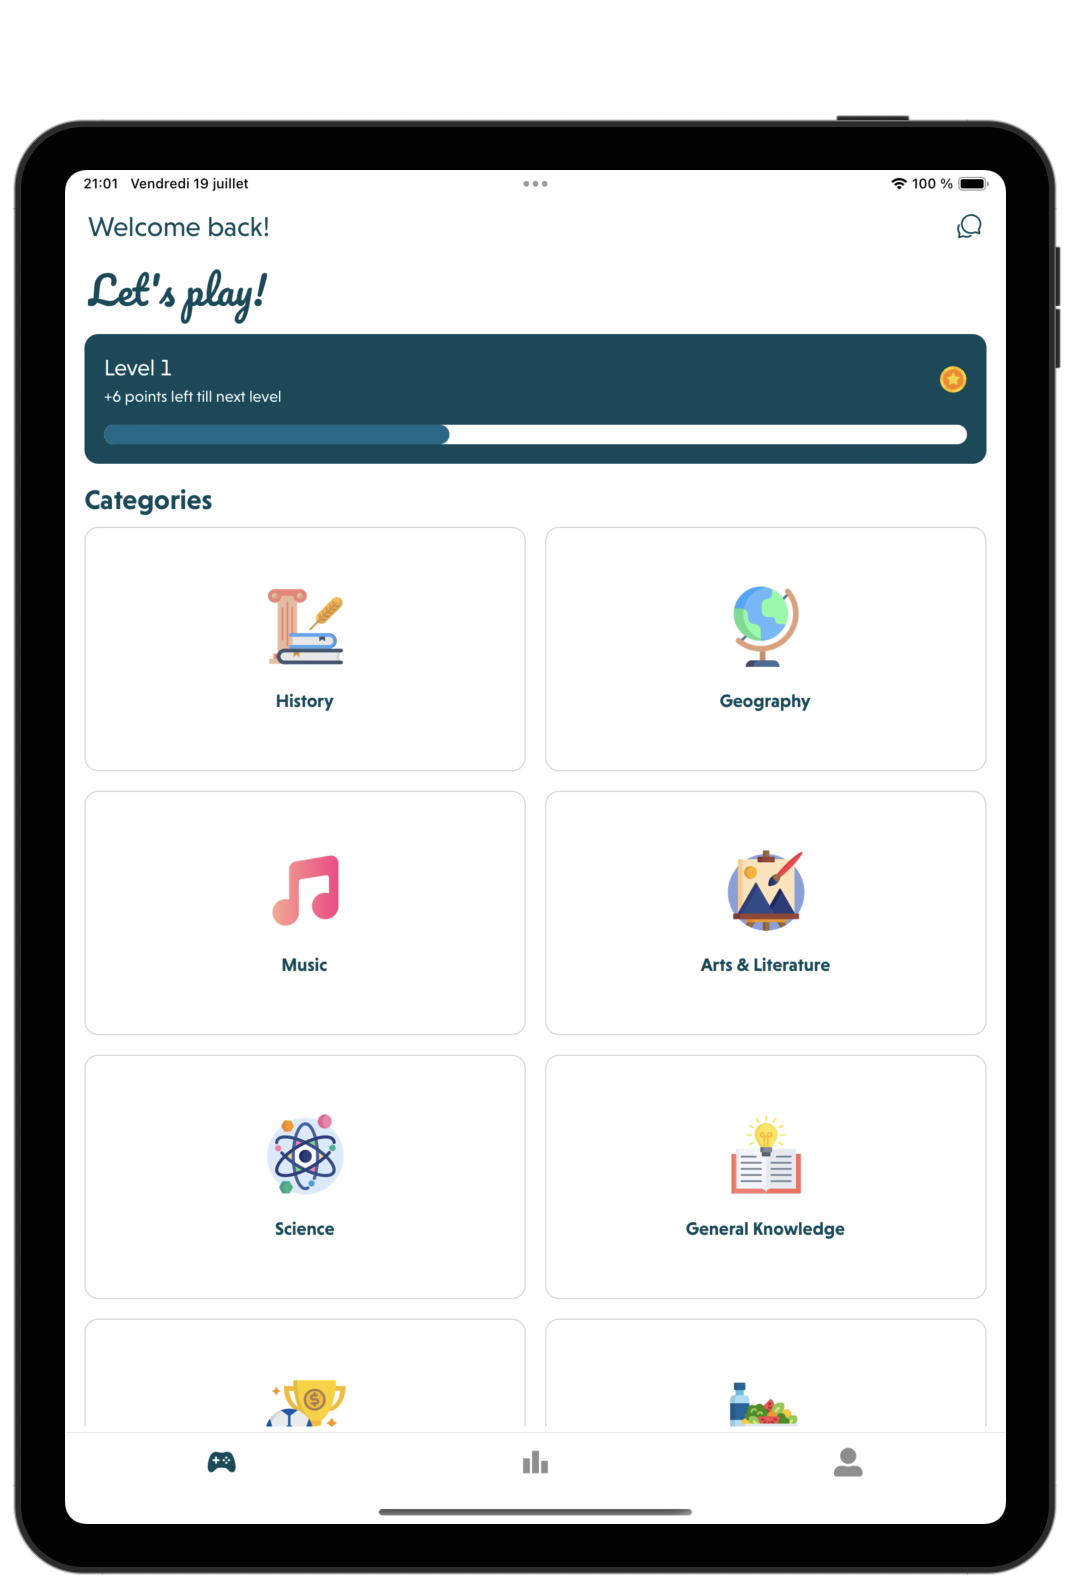
\includegraphics[height=10cm]{TabletUI/Quiz Page 1.png}
        \caption{Quiz Page 1}
    \end{minipage}
    \hspace{0.1\linewidth}
    \begin{minipage}[b]{0.43\linewidth}
        \centering
        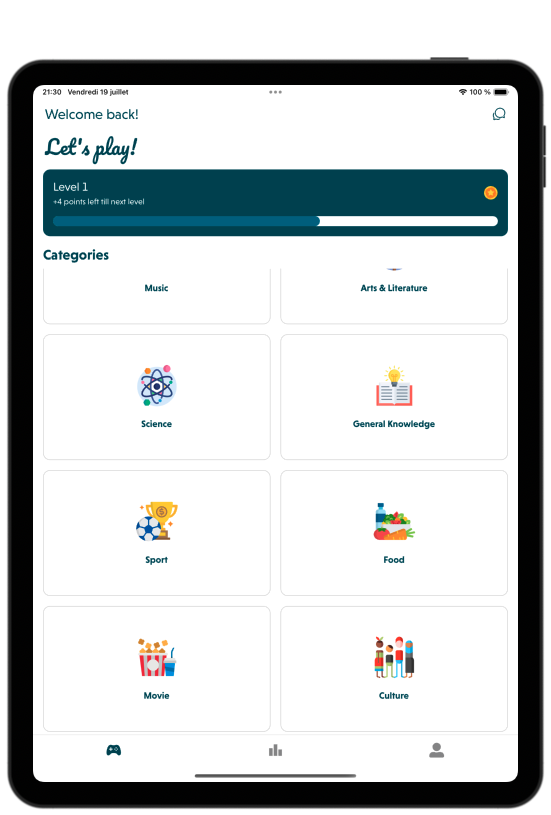
\includegraphics[height=10cm]{TabletUI/Quiz Page 2.png}
        \caption{Quiz Page 2}
    \end{minipage}
    \vspace{0.5cm}
    \caption{\textbf{The BrainMe Application All Quiz Categories}}
\end{figure}

The Ipad screen allows the user to have a more wider and bigger aspects of the icons and the text which is the major difference between the Iphone and the Ipad. The user here can select from various categories to begin the quiz.

\subsubsection{Quiz Levels}

\begin{figure}[H]
    \centering
    \begin{minipage}[b]{0.43\linewidth}
        \centering
        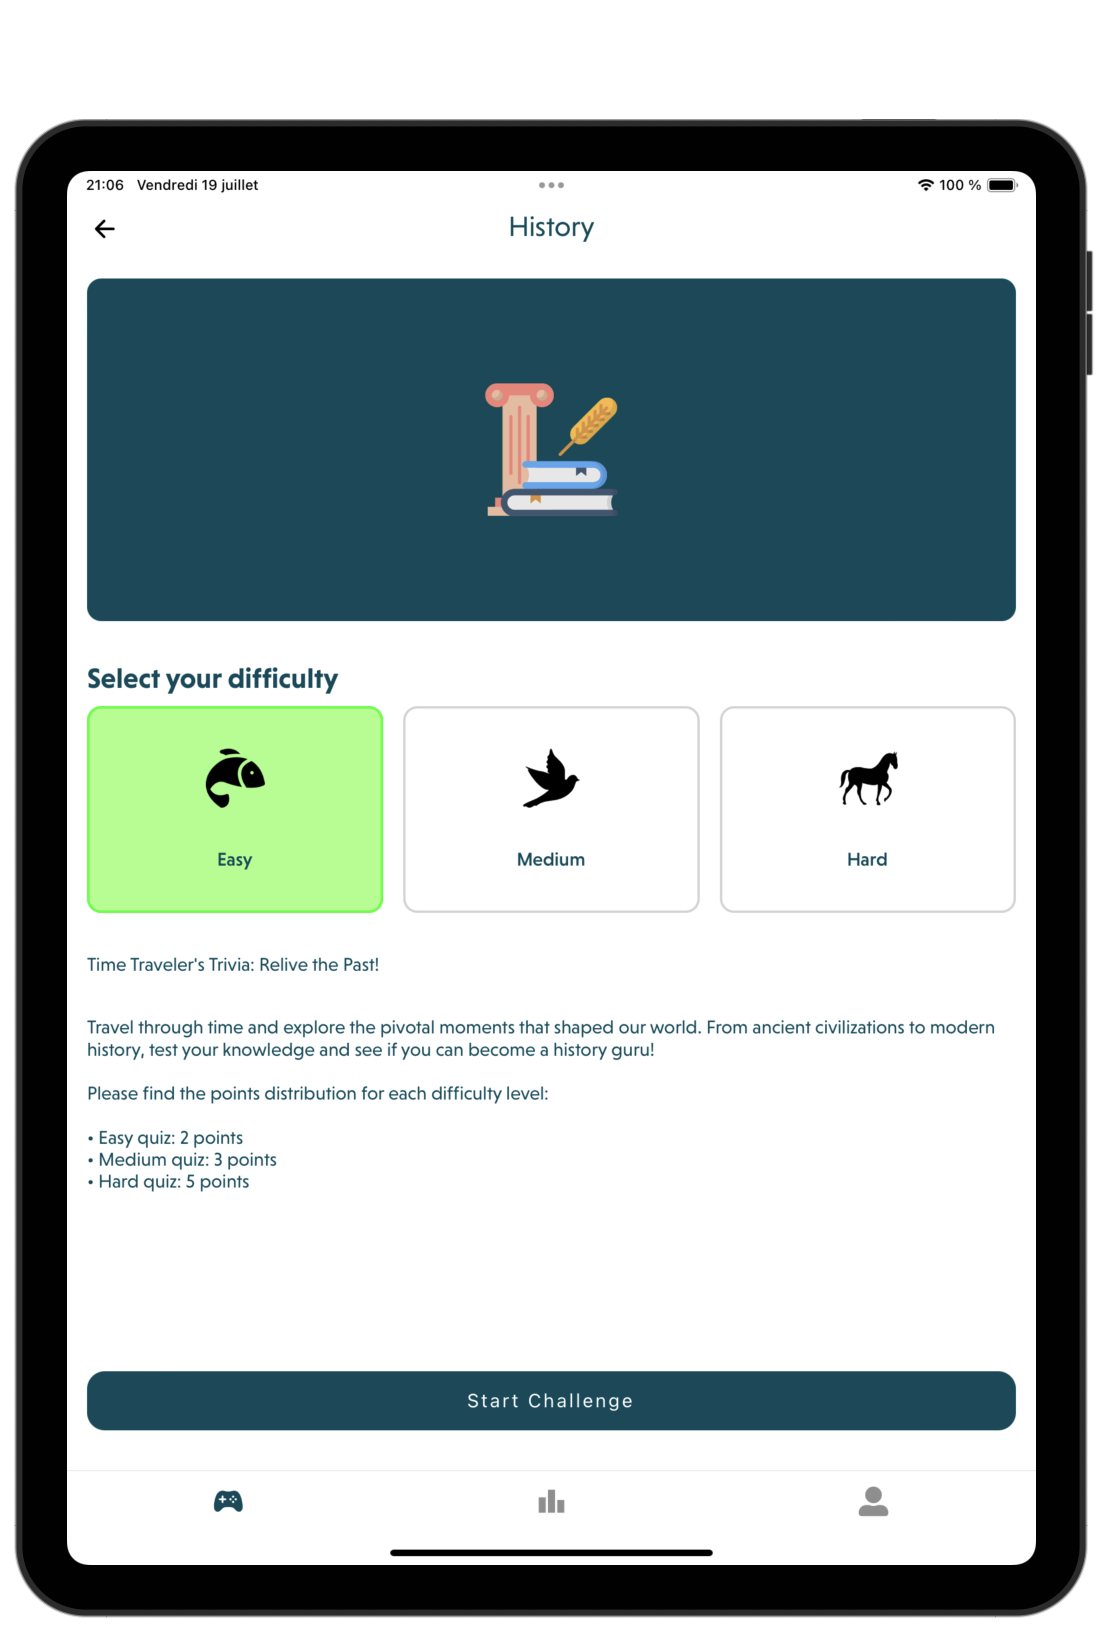
\includegraphics[height=10cm]{TabletUI/Easy Level Quiz.png}
        \caption{Easy Level Quiz}
    \end{minipage}
    \hspace{0.1\linewidth}
    \begin{minipage}[b]{0.43\linewidth}
        \centering
        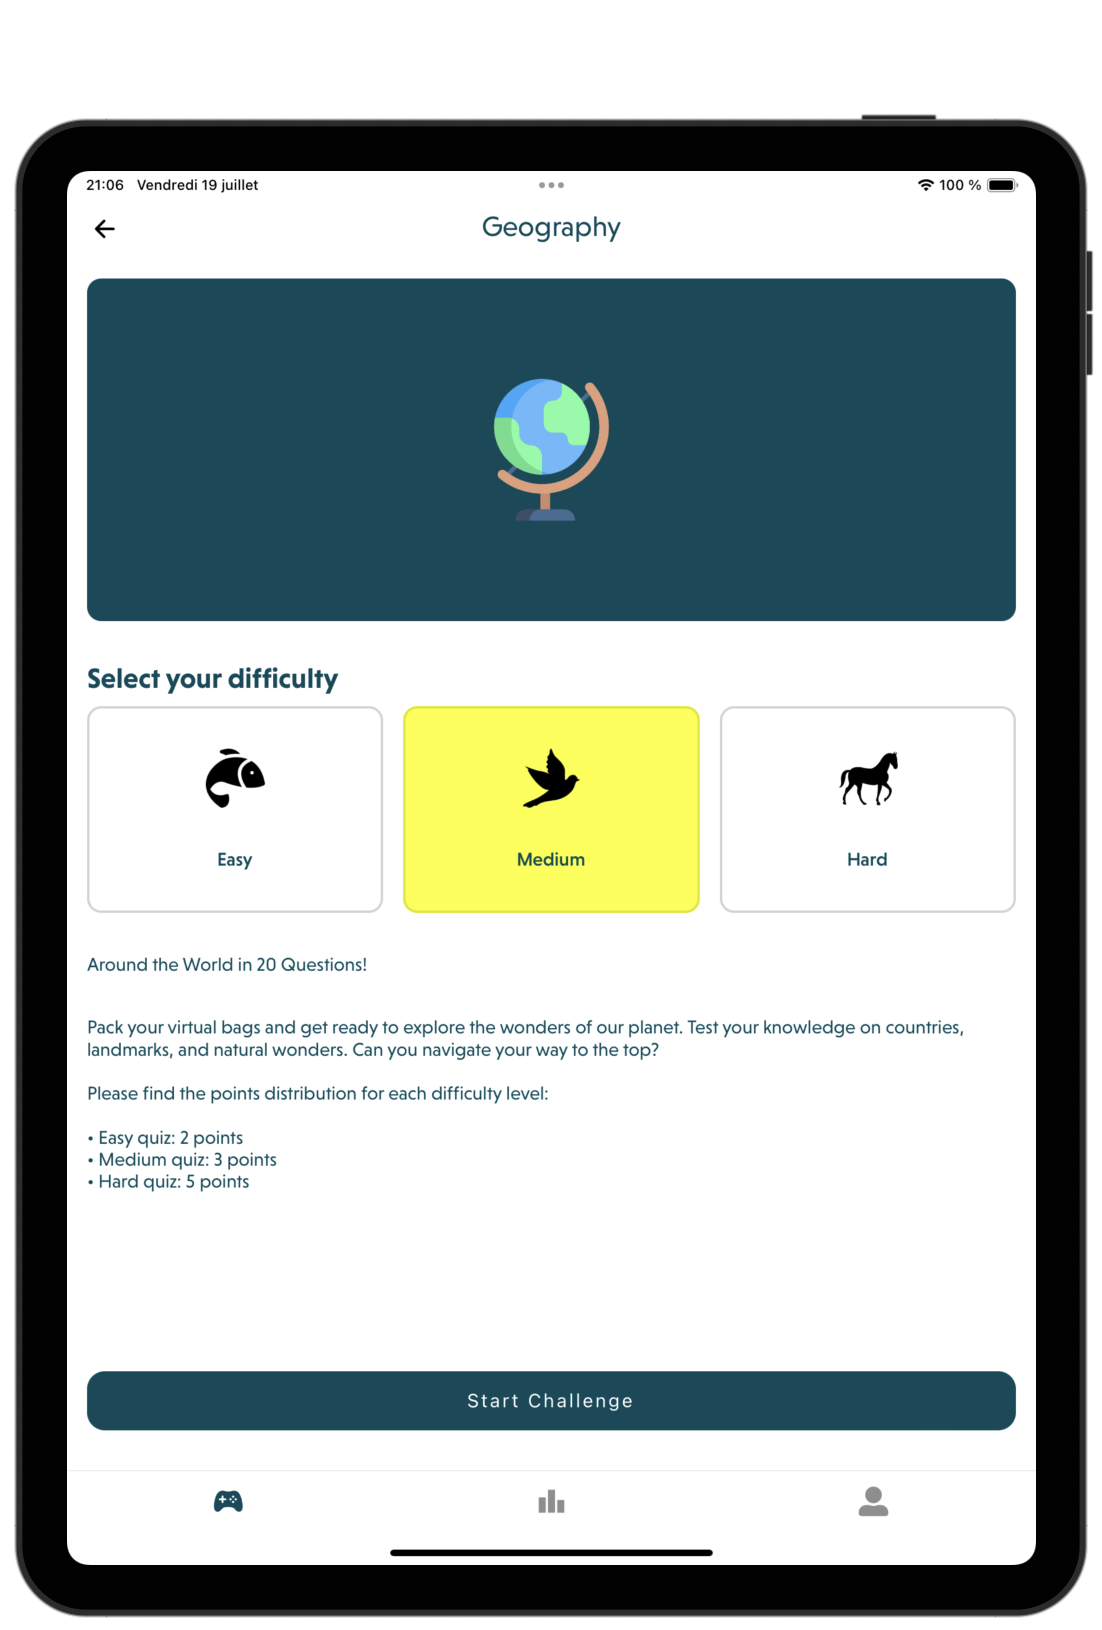
\includegraphics[height=10cm]{TabletUI/Medium Level Quiz.png}
        \caption{Medium Level Quiz}
    \end{minipage}
    \vspace{0.5cm}
    \caption{\textbf{Quiz Difficulty Description}}
\end{figure}

The above screen depicts the difficulty level the user can select from of different genres. THe user can select from easy medium and hard levels for the respective quiz and it will be more fun on Ipad or bigger screens to play or participate in the challenges.

\begin{figure}[H]
    \centering
    \begin{minipage}[b]{0.43\linewidth}
        \centering
        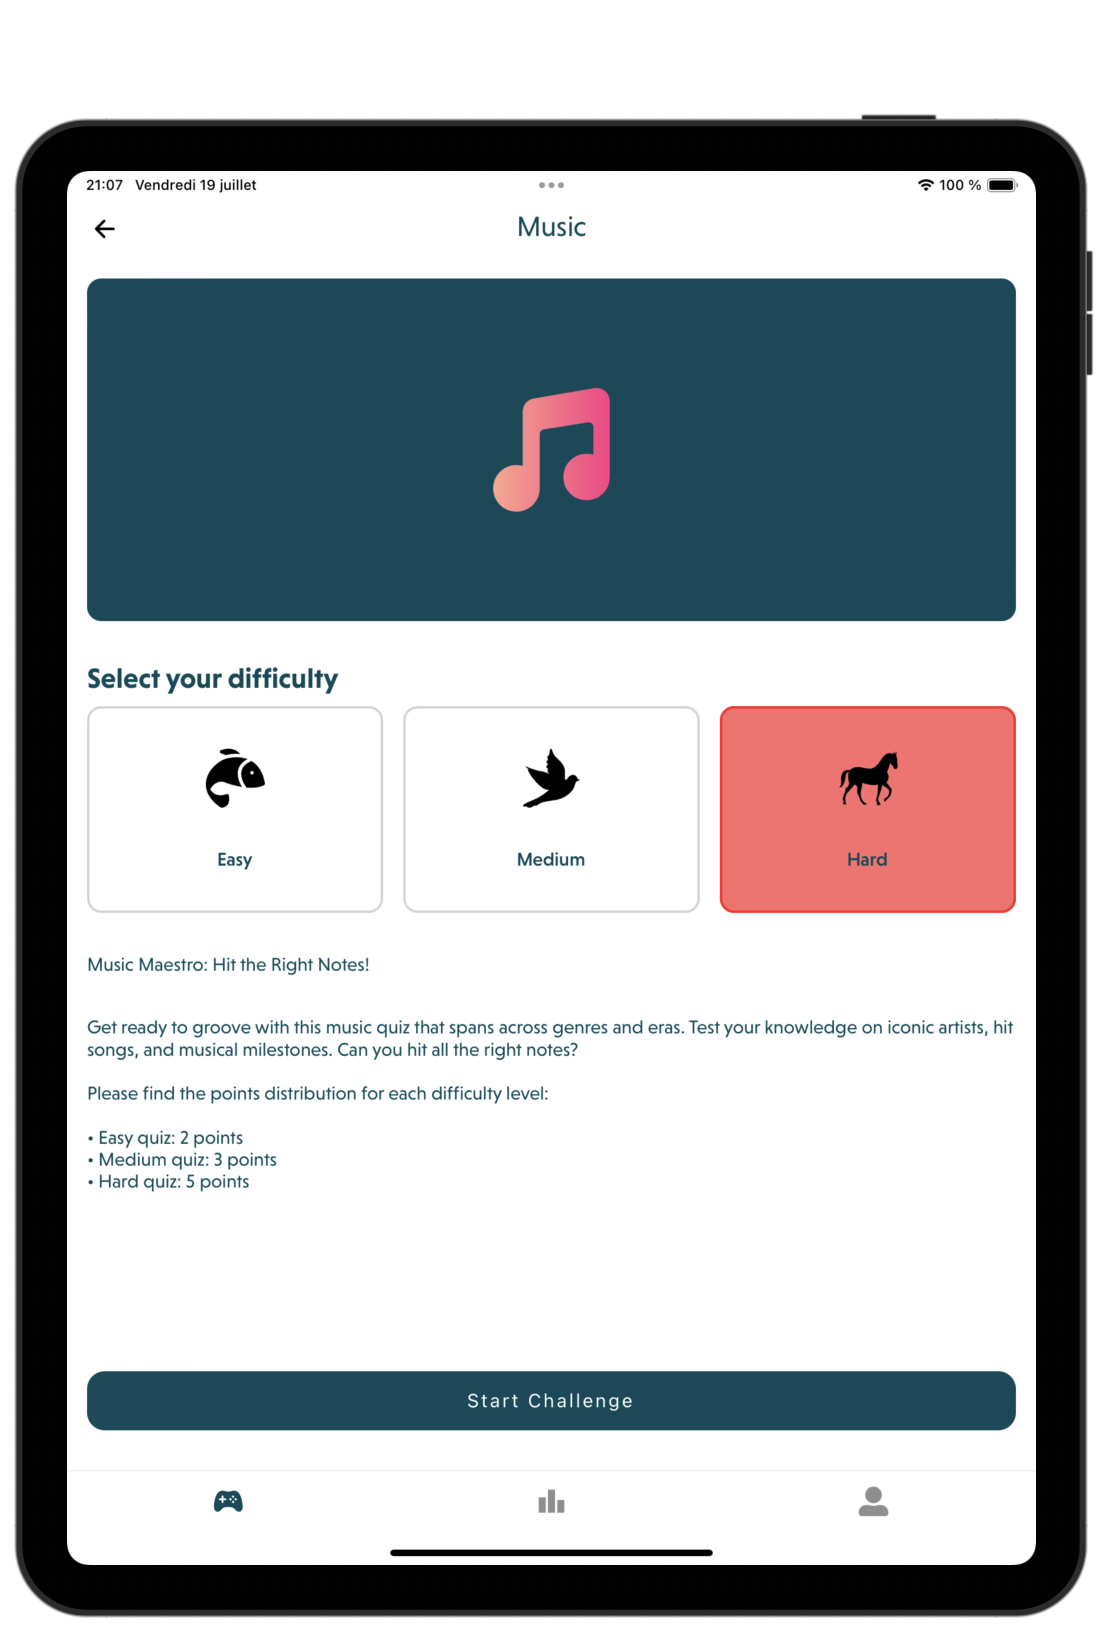
\includegraphics[height=10cm]{TabletUI/Hard Level Quiz.png}
        \caption{Hard Level Quiz}
    \end{minipage}
    \hspace{0.1\linewidth}
    \begin{minipage}[b]{0.43\linewidth}
        \centering
        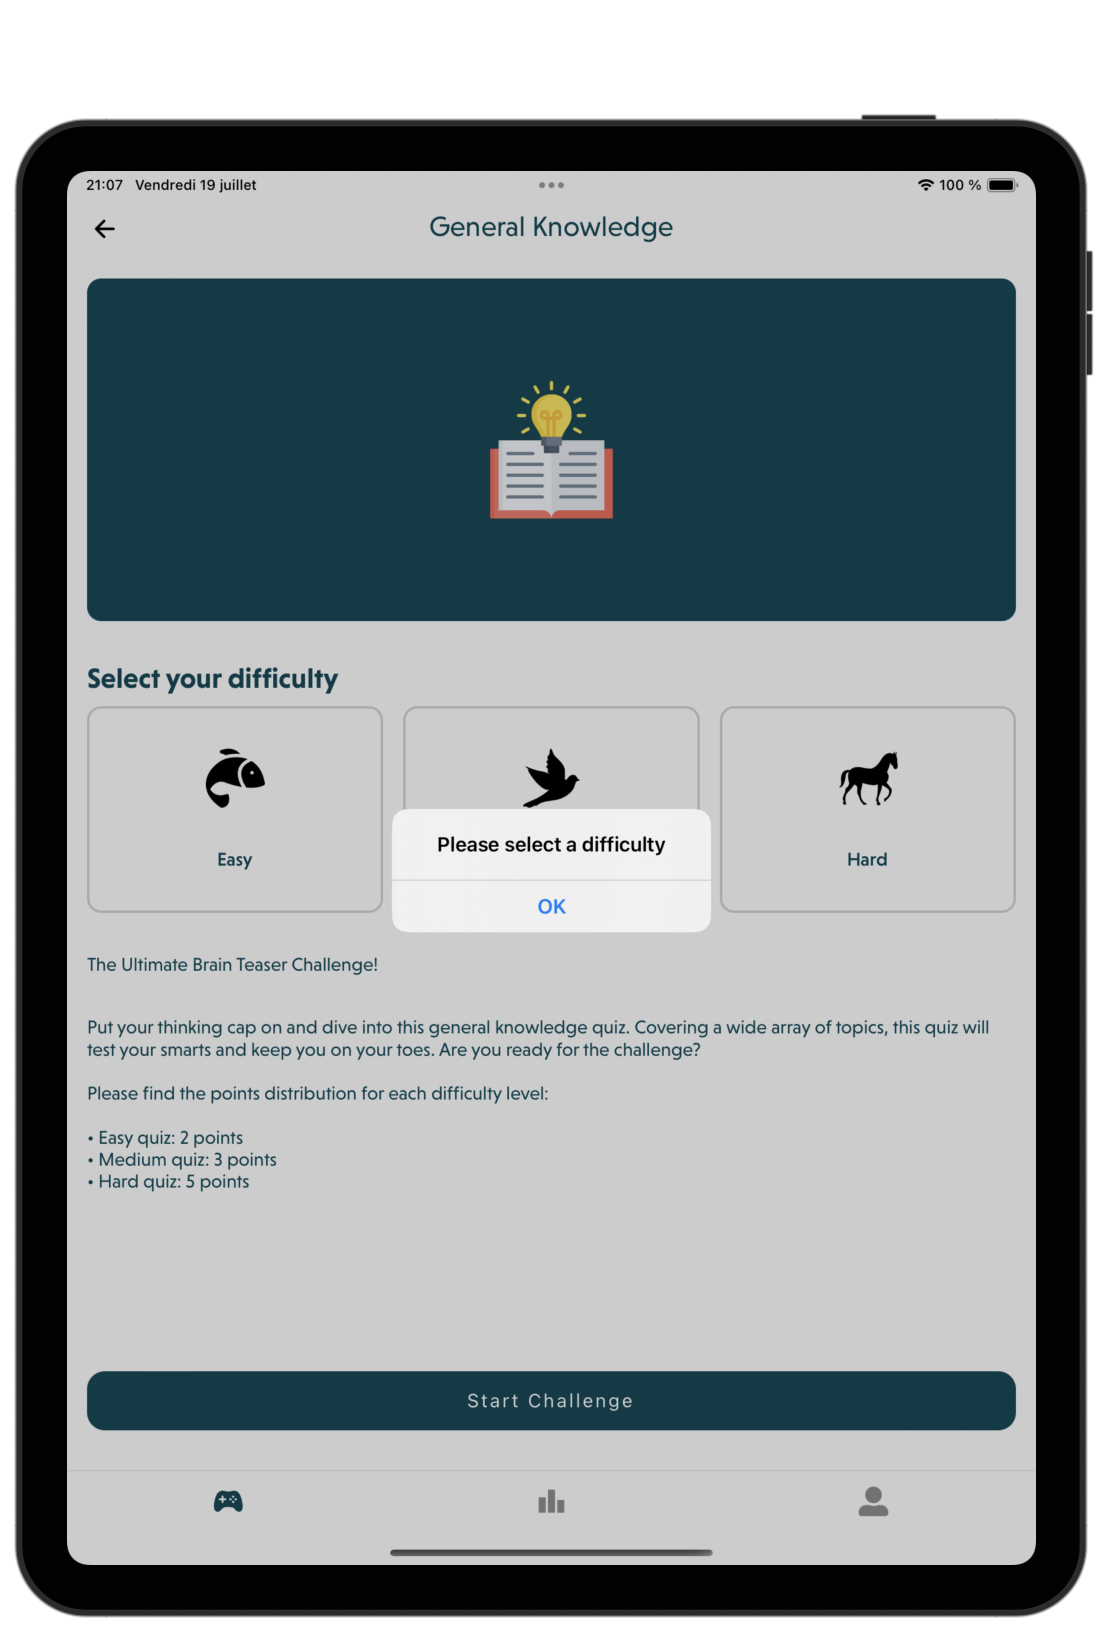
\includegraphics[height=10cm]{TabletUI/Select Difficulty.png}
        \caption{Select Difficulty}
    \end{minipage}
    \vspace{0.5cm}
    \caption{\textbf{Quiz Difficulty Description}}
\end{figure}

The user has to select a difficulty level in order to proceed. If the user does not make any selection, a alert box appears requesting the user to make a choice in order to proceed thus allowing more user engagement and making the application intuitive.

\subsubsection{Starting Quiz}

\begin{figure}[H]
    \centering
    \begin{minipage}[b]{0.43\linewidth}
        \centering
        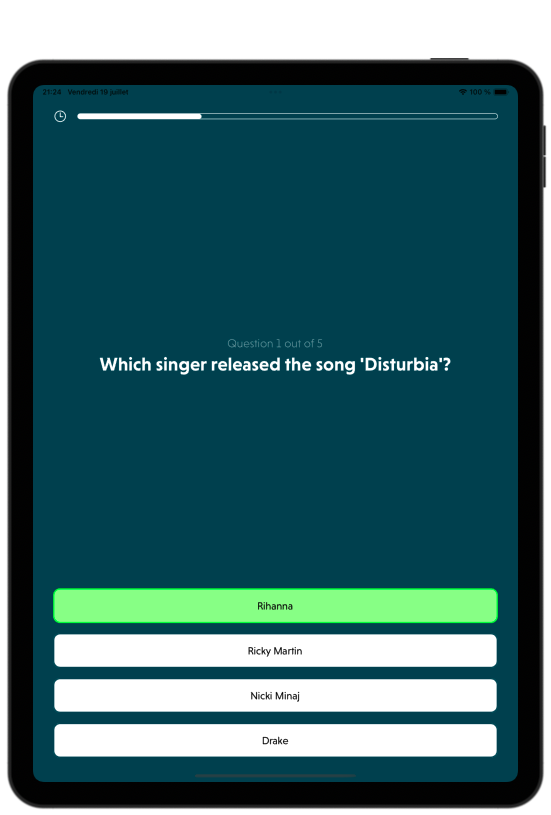
\includegraphics[height=10cm]{TabletUI/User selecting an option after starting a quiz.png}
        \caption{User selecting an option after starting a quiz}
    \end{minipage}
    \hspace{0.1\linewidth}
    \begin{minipage}[b]{0.43\linewidth}
        \centering
        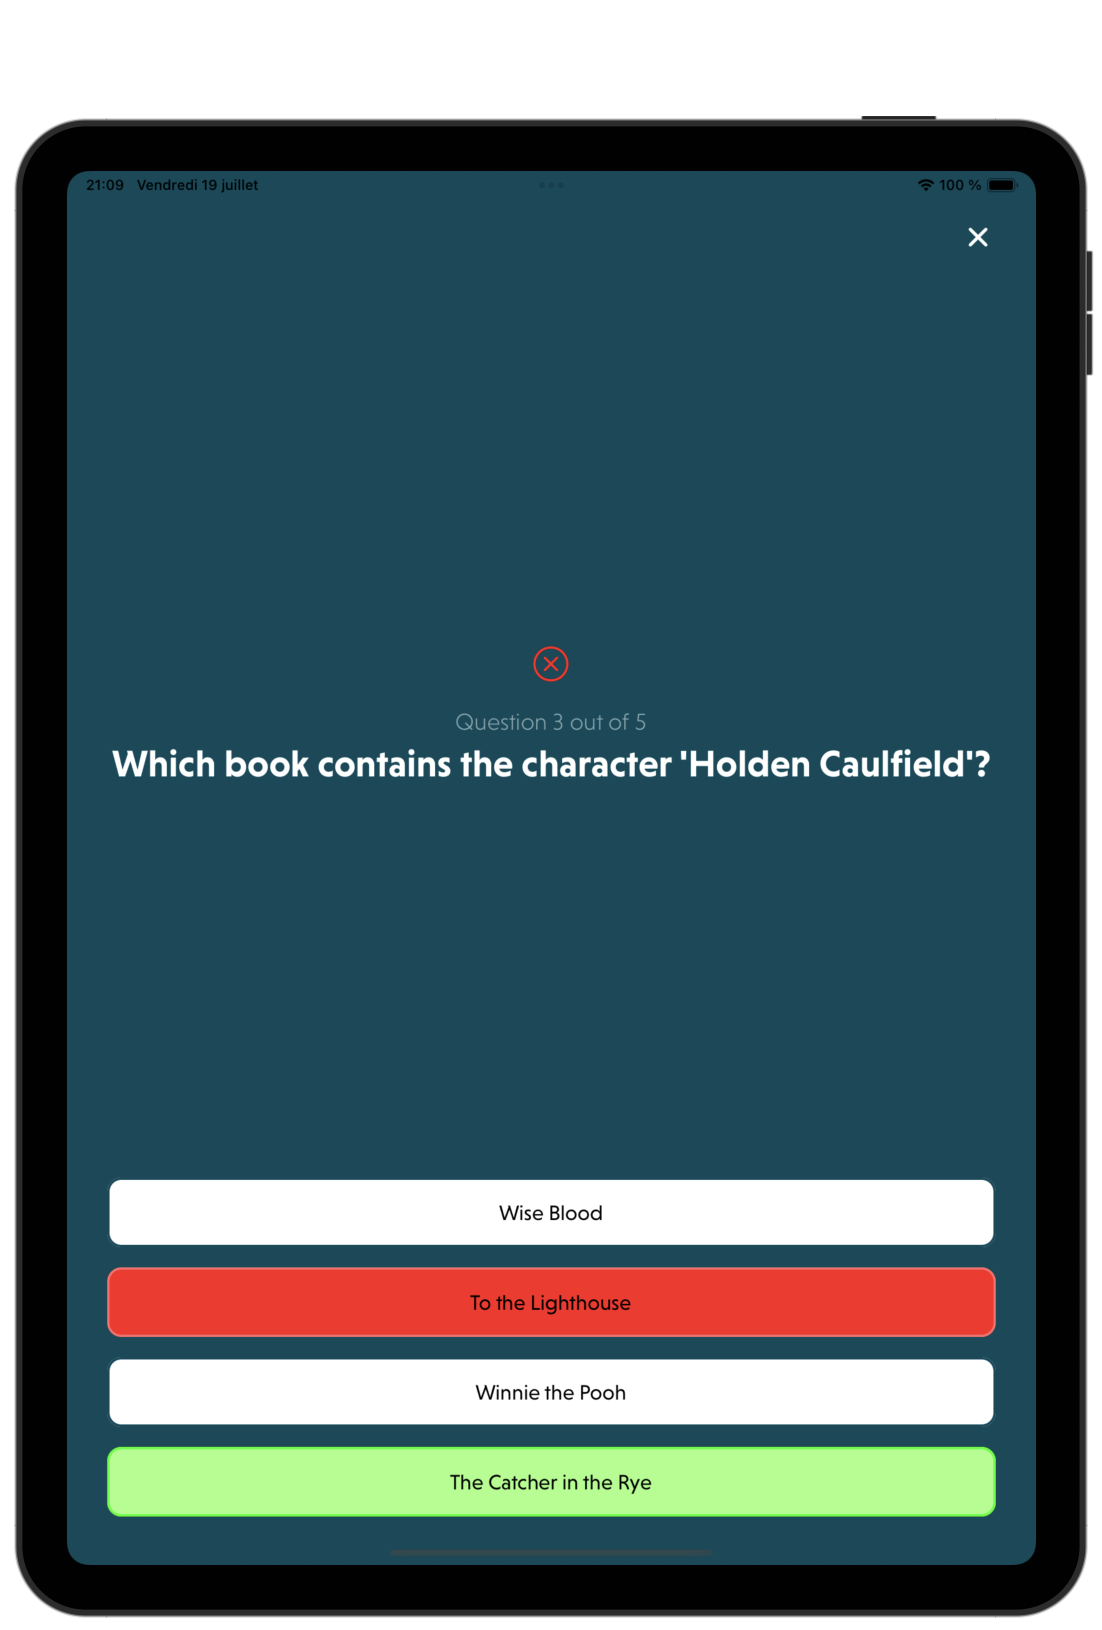
\includegraphics[height=10cm]{TabletUI/Showing the result after the time has ended.png}
        \caption{Showing the result after the time has ended}
    \end{minipage}
    \vspace{0.5cm}
    \caption{\textbf{Starting a quiz and selecting an option}}
\end{figure}

In this part of our application, just like the Iphone version, the user can start a quiz where the user gets 5 questions with a timer of 15 seconds and 4 options to select from based on the genre he has selected. Once the timer runs out, the user sees the solution if the choice made was correct or incorrect.

\subsubsection{Ending and Reviewing Quiz}

The ending and reviewing quiz screens provide users with a summary of their performance and an option to review their answers. These screens are designed to help users understand their mistakes and learn from them, enhancing the overall learning experience.

\begin{figure}[H]
    \centering
    \begin{minipage}[b]{0.43\linewidth}
        \centering
        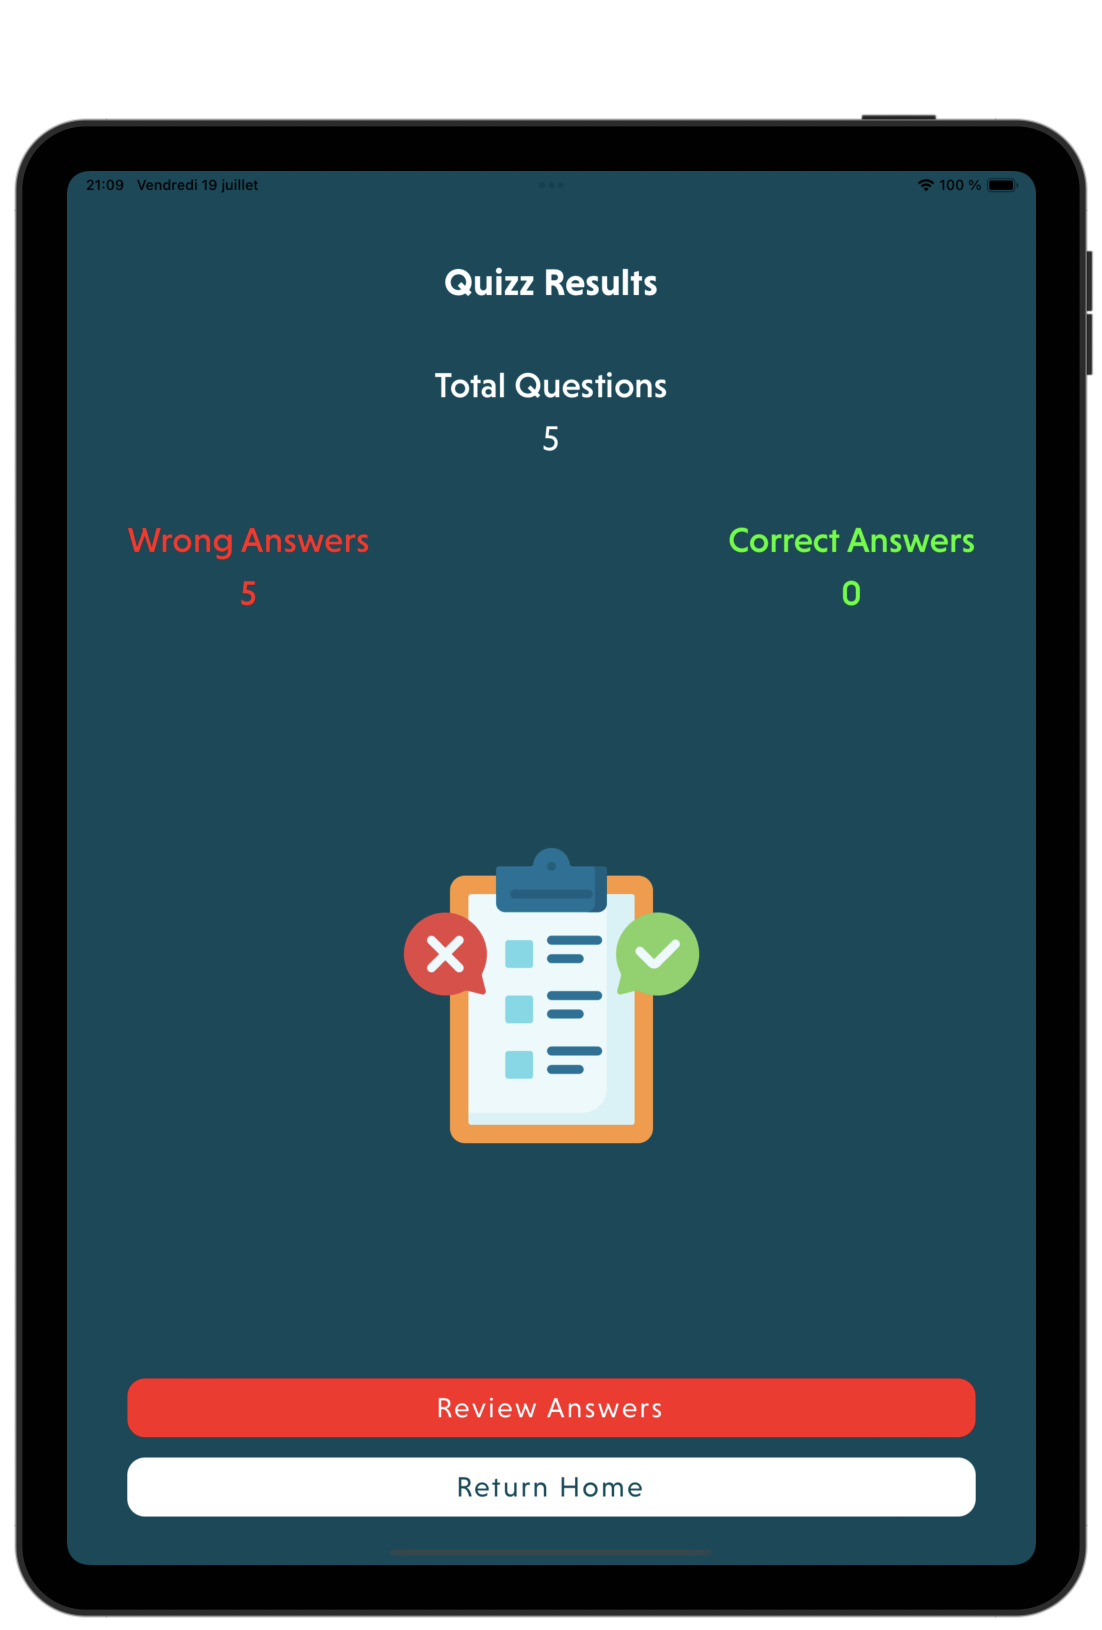
\includegraphics[width=\linewidth]{TabletUI/Quiz Results with options to review or return home.png}
        \caption{Quiz Results with options to review or return home}
    \end{minipage}
    \hspace{0.1\linewidth}
    \begin{minipage}[b]{0.43\linewidth}
        \centering
        \includegraphics[width=\linewidth]{TabletUI/Displaying correct result for incorrect solution.png}
        \caption{Displaying correct result for incorrect solution}
    \end{minipage}
    \vspace{0.5cm}
    \caption{\textbf{Ending a quiz and selecting an option}}
\end{figure}

The user has the option to review their answers by tapping the "Review Answers" button.
If the user chooses to review their answers:
    \begin{itemize}
        \item The quiz review screen displays each question along with the user's selected answer and the correct answer.
        \item Correct answers are highlighted in green icon, while incorrect answers are highlighted in red icon.
    \end{itemize}
The user can also choose to return to the home page by tapping the "Return Home" button. \\\\
The below images share a glimpse of how the user can review it. If the user has selected the correct option, a green tick appears on the top and if the user has made no selection, then a red cross appears on the top and the correct solution is displayed.

\begin{figure}[H]
    \centering
    \begin{minipage}[b]{0.43\linewidth}
        \centering
        \includegraphics[width=\linewidth]{TabletUI/Reviewing correct solution for correct solution.png}
        \caption{Reviewing correct solution for correct selection}
    \end{minipage}
    \hspace{0.1\linewidth}
    \begin{minipage}[b]{0.43\linewidth}
        \centering
        \includegraphics[width=\linewidth]{TabletUI/Reviewing correct solution for no selection.png}
        \caption{Reviewing correct solution for no selection}
    \end{minipage}
    \vspace{0.5cm}
    \caption{\textbf{Reviewing the correct result}}
\end{figure}


\vspace{1cm}

\subsubsection{Leaderboard}

The leaderboard feature in the BrainMe application displays the ranking of users based on their quiz performance. This promotes a competitive environment, motivating users to improve their scores and climb the ranks. Users can view their position relative to others, fostering a sense of achievement and encouraging active participation in quizzes.

\begin{figure}[H]
    \centering
    \begin{minipage}[b]{0.43\linewidth}
        \centering
        \includegraphics[width=\linewidth]{TabletUI/Leaderboard ranking depicting medals and rankings.png}
        \caption{Leaderboard ranking depicting medals and rankings}
    \end{minipage}
    \hspace{0.02\linewidth}
    \begin{minipage}[b]{0.43\linewidth}
        \centering
        \includegraphics[width=\linewidth]{TabletUI/Sliding on the name to chat or view profile.png}
        \caption{Sliding on the name to chat or view profile}
    \end{minipage}
    \caption{\textbf{Leaderboard ranking and the medals along with chat option}}
\end{figure}


\begin{itemize}
\item \textbf{Real-time updates:} The leaderboard is updated in real-time to reflect the latest user rankings based on quiz performance.
\item \textbf{Visual indicators:} Medals for the top three users provide immediate visual recognition of the leading participants.
\item \textbf{User details:} Displaying usernames and profile pictures makes the leaderboard more personal and engaging.
\item \textbf{Sliding feature} Allows registered users to send message or view their profile directly from the leaderboard rankings.
\item \textbf{Motivation and engagement:} The competitive nature of the leaderboard encourages users to participate more actively in quizzes to improve their ranking.
\end{itemize}

\subsubsection{Profile Page}

\begin{figure}[H]
    \centering
    \begin{minipage}[b]{0.43\linewidth}
        \centering
        \includegraphics[width=\linewidth]{TabletUI/User Profile UI with Statistics.png}
        \caption{\textbf{User Profile UI with Statistics}}
    \end{minipage}
\end{figure}


The Profile Page offers a comprehensive overview of the user's achievements and statistics within the BrainMe application. At the top, users can see their profile picture and username, providing a personalized touch. Below this, various statistics and achievements are displayed, including:

\begin{itemize}
\item \textbf{Leaderboard Rank:} Shows the user's current rank on the leaderboard, motivating them to improve their performance.
\item \textbf{Games Played:} Displays the total number of games the user has participated in.
\item \textbf{Points Total:} Indicates the total points accumulated by the user.
\item \textbf{Profile Level:} Represents the user's profile level based on their activity and achievements.
\item \textbf{Correct Answers:} Shows the percentage of questions the user has answered correctly.
\item \textbf{Incorrect Answers:} Displays the percentage of questions the user has answered incorrectly.
\end{itemize}

Additionally, there is a "Find Friends" button that allows users to search for and connect with other users within the app, enhancing the social learning experience. The clean and intuitive design ensures that users can easily access and understand their statistics, fostering a sense of achievement and encouraging continuous engagement with the app.

\subsubsection{Friend list and checking other user's profile}

\begin{figure}[H]
    \centering
    \begin{minipage}[b]{0.43\linewidth}
        \centering
        \includegraphics[width=\linewidth]{TabletUI/User's friends list.png}
        \caption{User's friends list}
    \end{minipage}
    \hspace{0.1\linewidth}
    \begin{minipage}[b]{0.43\linewidth}
        \centering
        \includegraphics[width=\linewidth]{TabletUI/Friend's User Profile.png}
        \caption{Friend's User Profile}
    \end{minipage}
    \vspace{0.5cm}
    \caption{\textbf{User's friend list along with friend's user profile}}
\end{figure}

The Friend List and Checking Other User's Profile feature in BrainMe enhances the social interaction aspect of the application. It allows users to view the friends they already follow and view their progress and achievements.

\begin{itemize}
\item \textbf{Friend List:} Users can see their friends' names, profile pictures, and the points they have earned. A search bar at the top allows users to quickly find specific friends by name.
\item \textbf{Friend's User Profile:} This shows a friend's detailed profile when selected from the friends list. The profile includes the friend's leaderboard rank, games played, total points, profile level, correct answer percentage, and incorrect answer percentage. Additionally, users can send a message or unfollow the friend using the buttons provided.
\end{itemize}

This feature promotes a competitive and collaborative environment, motivating users to improve their performance by comparing their achievements with those of their friends.

\subsubsection{Find Friends}

\begin{figure}[H]
    \centering
    \begin{minipage}[b]{0.43\linewidth}
        \centering
        \includegraphics[width=\linewidth]{TabletUI/Searching for a friend from the available users.png}
        \caption{Searching for a friend from the available users}
    \end{minipage}
    \hspace{0.1\linewidth}
    \begin{minipage}[b]{0.43\linewidth}
        \centering
        \includegraphics[width=\linewidth]{TabletUI/Filter search for following a friend.png}
        \caption{Filter search for following a friend}
    \end{minipage}
    \vspace{0.5cm}
    \caption{\textbf{User can search for a friend and follow them}}
\end{figure}

The Find Friends feature in BrainMe allows users to search for and connect with other users. This promotes social interaction and collaboration within the application.

\begin{itemize}
\item \textbf{Searching for a Friend:} The left screen shows the user entering a friend's name into the search bar. As the user types, the app filters the list to display matching names. This makes it easy for users to find specific friends quickly.
\item \textbf{Filter Search for Adding:} The right screen displays the results of the search, showing the user’s profile picture, name, and points. Users can select a friend from the list to view their profile and follow them.
\end{itemize}

\subsubsection{Chat Page}

\begin{figure}[H]
    \centering
    \begin{minipage}[b]{0.43\linewidth}
        \centering
        \includegraphics[width=\linewidth]{TabletUI/Creating a new chat.png}
        \caption{Creating new chat}
    \end{minipage}
    \hspace{0.1\linewidth}
    \begin{minipage}[b]{0.43\linewidth}
        \centering
        \includegraphics[width=\linewidth]{TabletUI/Chat System Example.png}
        \caption{Chat System Example}
    \end{minipage}
    \vspace{0.5cm}
    \caption{\textbf{Creation and an example of a new chat with file sharing}}
\end{figure}

The chat page allows users to create new chats and engage in conversations with other users. This feature supports both text and file sharing, enhancing the communication experience within the app.

\begin{itemize}
    \item \textbf{Creating New Chat:} Users can easily initiate a new chat with their friends by selecting from a list of contacts.
    \item \textbf{Chat System Example:} The chat interface displays messages exchanged between users, including the time stamps and any shared files.
    \item \textbf{File Sharing:} Users can share images and other files within the chat, making it more interactive and engaging.
\end{itemize}

\subsubsection{Settings Page}

\begin{figure}[H]
    \centering
    \begin{minipage}[b]{0.43\linewidth}
        \centering
        \includegraphics[width=\linewidth]{TabletUI/Account Settings Page.png}
        \caption{Account Settings Page}
    \end{minipage}
    \hspace{0.1\linewidth}
    \begin{minipage}[b]{0.43\linewidth}
        \centering
        \includegraphics[width=\linewidth]{TabletUI/Push Notifications.png}
        \caption{Push Notifications}
    \end{minipage}
    \vspace{0.5cm}
    \caption{\textbf{Account Settings with Push Notifications}}
\end{figure}

The Settings Page in BrainMe provides users with the ability to manage their account details and preferences, ensuring a personalized and secure experience. Users can choose to opt in or opt out of the push notifications and also update their profile image and other personal details.
\section{Testing Campaign}

In our testing campaign, we aimed to ensure that the BrainMe application is reliable, user-friendly, and functions correctly. We used various testing methods to cover different aspects of the application, including unit tests, widget tests, and coverage analysis. Here are the details:

\subsection{Testing Environment}

We set up a testing environment that mimics the real-world usage of the BrainMe application. This environment included:

\begin{itemize}
    \item \textbf{Devices}: We tested the application on iOS devices to ensure cross-platform compatibility.
    \item \textbf{Simulators}: We used simulators for different devices to perform automated tests.
    \item \textbf{Test Data}: We created realistic test data to simulate user interactions and scenarios.
    \item \textbf{Network Conditions}: We tested the app under various network conditions to ensure it performs well even with slow or unstable internet connections.
\end{itemize}

\subsection{Unit Test}

Unit tests are designed to test individual components of the application to ensure they work correctly. We focused on testing the smallest parts of the application, such as functions and methods.

\subsubsection{Goal of Unit Testing}

The goal of unit testing was to verify that each unit of the application performs as expected. This helps in identifying and fixing issues at an early stage of development.

\subsubsection{Steps We Followed}

\begin{enumerate}
    \item \textbf{Identify Units}: We identified the key units or functions in the application that needed testing.
    \item \textbf{Write Test Cases}: We wrote test cases for each unit to check its functionality.
    \item \textbf{Execute Tests}: We ran the test cases and recorded the results.
    \item \textbf{Fix Issues}: We fixed any issues that were identified during testing.
    \item \textbf{Repeat}: We repeated the tests to ensure the fixes were successful and did not introduce new issues.
\end{enumerate}

\subsection{Widget Test}

The aim of widget testing is to ensure that the user interface components of the BrainMe application are loaded and populated correctly. We used mock APIs to simulate data and verified through assertions that the widgets display the correct information. Our widget tests are structured to cover different screens and their respective use cases.

\subsubsection{Goal of Widget Testing}

The main goal of widget testing was to ensure that each widget in the application functions as expected and provides a good user experience. This involved verifying that the widgets render correctly with various data inputs and user interactions.

\subsubsection{Steps We Followed}

\begin{enumerate}
    \item \textbf{Identify Widgets}: We identified the key UI components that users interact with.
    \item \textbf{Write Test Scripts}: We wrote test scripts to simulate user interactions with these widgets.
    \item \textbf{Execute Tests}: We ran the test scripts to check the behavior of the widgets.
    \item \textbf{Analyze Results}: We reviewed the test results to identify any issues.
    \item \textbf{Fix Issues}: We fixed any issues found and re-ran the tests to ensure the fixes were effective.
\end{enumerate}

\subsubsection{Test Cases}

\begin{tabular}{|c|l|}
    \hline
    \textbf{Page Tested} & \textbf{Name of the Test (Description)} \\
    \hline
    Login/Registration & Check registration with correct input \\
    \hline
    Login/Registration & Check login with empty input \\
    \hline
    Login/Registration & Check login with correct input \\
    \hline
    Login/Registration & Check forget password \\
    \hline
    Login/Registration & Check registration with empty input \\
    \hline
    Login/Registration & Check registration with wrong input \\
    \hline
    Quiz Page & Check render if no quiz available \\
    \hline
    Quiz Page & Check render if quizzes are available \\
    \hline
    Quiz Page & Check render of all quiz types \\
    \hline
    Quiz Page & Check quiz submission \\
    \hline
    Leaderboard & Check initial render screen \\
    \hline
    Leaderboard & Check render if no scores found \\
    \hline
    Leaderboard & Check render if scores found \\
    \hline
    Profile & Check initial render \\
    \hline
    Profile & Check render if no data available \\
    \hline
    Profile & Check render with user data \\
    \hline
    Profile & Check edit profile functionality \\
    \hline
    Settings & Check initial render \\
    \hline
    Settings & Check toggle notifications \\
    \hline
    Settings & Check change password functionality \\
    \hline
    Settings & Check delete account functionality \\
    \hline
\end{tabular}

\vspace{1cm}

Each test case ensured that the specific components of the BrainMe application functioned correctly when tested. By following this process, we efficiently identified and resolved issues, ensuring the application was reliable and user-friendly.

\subsubsection{Coverage Analysis}

Coverage analysis is used to measure how much of the code is executed during testing. This helps in identifying untested parts of the code.

\subsubsection{Goal of Coverage Analysis}

The goal of coverage analysis was to ensure that our tests cover a significant portion of the code, helping us to identify areas that need more testing.

\subsubsection{Steps We Followed}

\begin{enumerate}
    \item \textbf{Run Tests}: We ran our unit and widget tests.
    \item \textbf{Generate Coverage Report}: We used tools to generate a coverage report that shows the percentage of code covered by tests.
    \item \textbf{Analyze Report}: We analyzed the report to identify untested parts of the code.
    \item \textbf{Write Additional Tests}: We wrote additional tests to cover the untested parts.
    \item \textbf{Repeat}: We repeated the process until we achieved at least 80\% code coverage.
\end{enumerate}

\subsubsection{Coverage Report}

\textbf{Below is the average coverage report}

\begin{figure}[H]
    \centering
    \includegraphics[width=1\linewidth, height=0.4\textheight]{Images/Coverage Report.png}
    \caption{Test Coverage Report}
\end{figure}


The above table shows the coverage for each file, indicating the percentage of statements, branches, functions, and lines that are covered by tests. \\\\
We followed the same process unless every component was tested and the coverage was above 80\% for all the components.

\vspace{1cm}

\textbf{Here is our Final Test coverage report results for all the components :}

\begin{figure}[H]
    \centering
    \includegraphics[width=1\linewidth, height=0.15\textheight]{Images/Test Results.png}
    \caption{Test Coverage Report}
\end{figure}

\textbf{Few examples of how we tested and what parts: }

\begin{figure}[H]
    \centering
    \includegraphics[width=1\linewidth, height=0.4\textheight]{Images/Test Results Example.png}
    \caption{Test Coverage Examples}
\end{figure}

By following these detailed steps in our testing campaign, we ensured that the BrainMe application is robust, reliable, and user-friendly.

\subsection{Automatic Testing}

We performed automatic testing to ensure that the BrainMe application functions correctly without manual intervention. Our goal was to achieve at least 80\% coverage. Automatic testing helped us quickly identify and fix issues, saving time and improving the reliability of the application.

\subsubsection{Goal of Automatic Testing}

The main goal of automatic testing was to validate that all parts of the application work as expected when executed automatically. We focused on:
\begin{itemize}
    \item Ensuring consistent and repeatable tests.
    \item Identifying defects quickly.
    \item Reducing the time and effort required for manual testing.
\end{itemize}

\subsubsection{Steps We Followed}

\begin{enumerate}
    \item \textbf{Select Testing Framework}: We chose Detox for end-to-end testing of our React Native application.
    \item \textbf{Write Test Scripts}: We wrote test scripts in TypeScript for various components of the application.
    \item \textbf{Set Up Test Environment}: We set up an environment where tests could run automatically.
    \item \textbf{Execute Tests}: We ran the test scripts automatically to check the functionality of different components.
    \item \textbf{Analyze Results}: We reviewed the test results to identify and fix any defects.
    \item \textbf{Repeat Tests}: We repeated the tests after fixing issues to ensure that the application works correctly.
\end{enumerate}

\subsubsection{Test Cases}

\begin{tabular}{|c|l|}
    \hline
    \textbf{Test Case ID} & \textbf{Description} \\
    \hline
    Test Case 1 & Automatically test the Login functionality. \\
    \hline
    Test Case 2 & Automatically test the Registration process. \\
    \hline
    Test Case 3 & Automatically test the Quiz feature. \\
    \hline
    Test Case 4 & Automatically test the Leaderboard functionality. \\
    \hline
    Test Case 5 & Automatically test the Profile management. \\
    \hline
    Test Case 6 & Automatically test the Settings adjustments. \\
    \hline
    Test Case 7 & Automatically test the overall user workflow from Login to Leaderboard. \\
    \hline
\end{tabular}

\vspace{1cm}

Each test case ensured that the specific components of the BrainMe application functioned correctly when tested automatically. By following this process, we efficiently identified and resolved issues, ensuring the application was reliable and user-friendly.

\subsubsection{Continuous Integration and Continuous Deployment (CI/CD)}

To streamline our development process, we integrated automatic testing with GitHub CI/CD. This ensured that our tests run every time we push code changes to the repository, helping us maintain code quality and reliability.

\begin{enumerate}
    \item \textbf{Set Up GitHub Actions}: We created a GitHub Actions workflow to automate the testing process.
    \item \textbf{Configure Workflow}: We configured the workflow to run Detox tests on every push and pull request.
    \item \textbf{Run Tests}: GitHub Actions automatically runs the tests and provides feedback on the test results.
    \item \textbf{Deploy on Success}: If all tests pass, the application is automatically deployed to the staging environment.
\end{enumerate}

\subsubsection{GitHub Actions Workflow}

Here is an example of the GitHub Actions workflow file we used:

\begin{verbatim}
name: CI/CD Pipeline

on: [push, pull_request]

jobs:
  build:
    runs-on: ubuntu-latest
    steps:
    - uses: actions/checkout@v2
    - name: Set up Node.js
      uses: actions/setup-node@v2
      with:
        node-version: '14'
    - name: Install dependencies
      run: npm install
    - name: Run tests
      run: npm test
    - name: Run Detox tests
      run: npm run test:detox
\end{verbatim}

This workflow checks out the code, sets up Node.js, installs dependencies, runs unit tests, and then runs Detox tests. If all tests pass, it proceeds to deployment. \\\\
By integrating automatic testing and CI/CD, we ensured that the BrainMe application remains stable and reliable, providing a seamless experience for our users.


\subsubsection{Goal of Integration Testing}

The main goal of our integration testing was to validate the interactions between the individual modules and to ensure that they function correctly when combined. We focused on:
\begin{itemize}
\item Ensuring that data flows correctly between modules.
\item Identifying and resolving interface defects.
\item Verifying that the integrated system meets the specified requirements.
\end{itemize}

\subsubsection{Steps We Followed}

\begin{enumerate}
\item \textbf{Identify Top-Level Components}: We started with the top-level component of the BrainMe application.
\item \textbf{Prepare Stubs for Lower-Level Components}: We created stubs for lower-level components that were not yet integrated.
\item \textbf{Develop Test Cases}: We wrote test cases to check the interactions between components.
\item \textbf{Execute Tests}: We integrated the top-level component with the stubs and ran the test cases.
\item \textbf{Integrate Lower-Level Components}: We replaced the stubs with actual lower-level components incrementally and continued testing.
\item \textbf{Repeat Until All Components are Integrated}: We continued this process until all components were integrated and tested.
\item \textbf{Validate Overall System Functionality}: We performed comprehensive testing to ensure that all components interact correctly and the overall system functions as expected.
\end{enumerate}

\subsubsection{Test Cases}

\begin{longtable}{|c|p{10cm}|}
\hline
\textbf{Test Case ID} & \textbf{Description} \\
\hline
Test Case 1 & Verify the functionality of the Login component with stubs for Registration and Dashboard. \\
\hline
Test Case 2 & Verify the functionality of the Login and Registration components with stubs for Quiz and Leaderboard. \\
\hline
Test Case 3 & Verify the functionality of Login, Registration, and Quiz components with stubs for Leaderboard and Profile. \\
\hline
Test Case 4 & Verify the functionality of Login, Registration, Quiz, and Leaderboard components with stubs for Profile and Settings. \\
\hline
Test Case 5 & Verify the functionality of Login, Registration, and Dashboard with stubs for Quiz and Settings. \\
\hline
Test Case 6 & Verify the functionality of Login, Registration, Dashboard, and Quiz components with stubs for Profile and Settings. \\
\hline
Test Case 7 & Verify the functionality of Login, Registration, Dashboard, Quiz, Profile, and Settings components. \\
\hline
\end{longtable}

Each test case ensured that the integrated components interacted correctly and met the expected requirements. Through this rigorous testing process, we achieved our goal of ensuring that the BrainMe application functions seamlessly as a cohesive system.

\subsection{User Test}

We conducted user tests with eight participants from diverse backgrounds to gather feedback on BrainMe. Each participant tested the application from installation to the leaderboard and provided detailed feedback on their experiences. Here are the results:

\subsubsection{Chiara Bottazzini: Bocconi Student, 24y, Female, Economics (CEMS)}

\begin{itemize}
    \item \textbf{Installation:} Chiara found the installation process smooth and straightforward. She appreciated the clear instructions provided.
    \item \textbf{Login and Registration:} She easily registered using her email and was able to log in without any issues. 
    \item \textbf{Quiz Experience:} Chiara enjoyed the quiz topics related to economics. She found the questions challenging but fair. 
    \item \textbf{Leaderboard:} The leaderboard was motivating for her. She liked seeing her rank compared to her peers.
    \item \textbf{Feedback:} Chiara mentioned that the user interface could be improved for better visual appeal. She also suggested adding more quiz topics related to her field.
\end{itemize}

\subsubsection{Thibault Beineix: HEC Student, 26, Male, Entrepreneurship}

\begin{itemize}
    \item \textbf{Installation:} Thibault found the app easy to download and install. The process was quick and hassle-free.
    \item \textbf{Login and Registration:} He registered using his email but faced a slight delay during the verification process.
    \item \textbf{Quiz Experience:} Thibault enjoyed the entrepreneurship quizzes. He found the questions engaging and relevant to his studies.
    \item \textbf{Leaderboard:} The leaderboard feature was exciting for him. It encouraged him to participate more actively.
    \item \textbf{Feedback:} Thibault suggested improving the speed of the email verification process. He also recommended adding more interactive elements in the quizzes.
\end{itemize}

\subsubsection{Maxime Limagne: EasyJet Pilot Student, 25, Male, Pilot Apprentice}

\begin{itemize}
    \item \textbf{Installation:} Maxime experienced a seamless installation process with no issues.
    \item \textbf{Login and Registration:} He registered quickly using his email and appreciated the straightforward process.
    \item \textbf{Quiz Experience:} Maxime did not find the aviation-related quizzes very strange. He enjoyed testing his knowledge in other fields field.
    \item \textbf{Leaderboard:} The leaderboard was a great addition for him, as it added a competitive edge to his learning.
    \item \textbf{Feedback:} Maxime suggested adding more aviation-specific content. He also mentioned that the app could benefit from a darker theme option for night use.
\end{itemize}

\subsubsection{Solène Marache: Bocconi Student, 26, Female, Economics (CEMS)}

\begin{itemize}
    \item \textbf{Installation:} Solène found the installation process easy and user-friendly.
    \item \textbf{Login and Registration:} She registered without any problems and found the login process smooth.
    \item \textbf{Quiz Experience:} Solène appreciated the variety of quiz topics available. She found the questions well-structured and informative.
    \item \textbf{Leaderboard:} The leaderboard was motivating for her, and she liked the idea of competing with friends.
    \item \textbf{Feedback:} Solène suggested adding more detailed explanations for quiz answers. She also recommended improving the app's speed during peak usage times.
\end{itemize}

\subsubsection{Romain Lafrance: Bocconi Student, 26, Male, Economics (CEMS)}

\begin{itemize}
    \item \textbf{Installation:} Romain had no issues with the installation process and found it quick.
    \item \textbf{Login and Registration:} He registered easily but felt the password requirements were a bit too strict.
    \item \textbf{Quiz Experience:} Romain enjoyed the quizzes but he particularly did not find those related to economics. He found the rest challenging and educational.
    \item \textbf{Leaderboard:} The leaderboard was a great motivator for him. He liked seeing his progress compared to others.
    \item \textbf{Feedback:} Romain suggested relaxing the password requirements slightly. He also recommended adding more interactive elements to the quizzes.
\end{itemize}

\subsubsection{Luigi d’Andria: Luiss School Student, 24, Male, HR Department}

\begin{itemize}
    \item \textbf{Installation:} Luigi found the installation process straightforward and efficient.
    \item \textbf{Login and Registration:} He registered quickly and appreciated the clear instructions provided.
    \item \textbf{Quiz Experience:} Luigi did not find HR-related quizzes. He found the remaining topics to be challenging and informative He found the questions relevant and well-formulated.
    \item \textbf{Leaderboard:} The leaderboard feature was motivating for him. He liked the competitive aspect it added.
    \item \textbf{Feedback:} Luigi suggested adding more HR-specific content. He also mentioned that the app could benefit from a more modern design.
\end{itemize}

\subsubsection{Dario Bagnoli: Luiss School Student, 26, Male, HR Department}

\begin{itemize}
    \item \textbf{Installation:} Dario experienced a smooth installation process with no issues.
    \item \textbf{Login and Registration:} He registered without any problems and found the login process straightforward.
    \item \textbf{Quiz Experience:} Dario did not find HR-related quizzes. He found the remaining topics to be challenging and informative.
    \item \textbf{Leaderboard:} The leaderboard was motivating for him, and he liked competing with his peers.
    \item \textbf{Feedback:} Dario suggested adding more detailed explanations for quiz answers. He also recommended improving the app’s speed during peak usage times.
\end{itemize}

\subsubsection{Adrian Valica: EPFL, 20, Male, Computer Science Student}

\begin{itemize}
    \item \textbf{Installation:} Adrian found the installation process easy and quick.
    \item \textbf{Login and Registration:} He registered using his email and appreciated the smooth process.
    \item \textbf{Quiz Experience:} Adrian enjoyed the computer science quizzes. He found the questions challenging and relevant to his studies.
    \item \textbf{Leaderboard:} The leaderboard feature was exciting for him. It encouraged him to participate more actively.
    \item \textbf{Feedback:} Adrian suggested adding more advanced computer science topics. He also recommended enhancing the app’s design for better user experience.
\end{itemize}

\section{Future Developments}

We're always working to make BrainMe better! Here are some exciting changes coming soon:

\begin{itemize}
    \item \textbf{Personalized Learning Paths}: We'll use smart algorithms to create customized learning plans just for you, based on your progress and interests.
    \item \textbf{Virtual Study Groups}: Join live study sessions with other users, work on problems together, and share resources in real-time.
    \item \textbf{More Language Support}: We'll add more languages to the app, so users from around the world can learn in their native language.
    \item \textbf{Offline Learning}: Download courses and quizzes to learn offline, and we'll sync your progress when you're back online.
    \item \textbf{Improved User Interface}: We'll make the app look and feel better, with updates based on your feedback.
    \item \textbf{Advanced Analytics}: Get detailed insights into your learning progress, strengths, and areas for improvement to help you optimize your study habits.
    \item \textbf{Gamification Updates}: We'll add new badges, rewards, and leaderboards to make learning more fun and engaging.
    \item \textbf{Peer Review and Feedback}: Get feedback from other users on your quizzes and assignments, and learn from each other's strengths and weaknesses.
    \item \textbf{Live Support Chat}: Get immediate help and support from our team through a live chat feature.
    \item \textbf{New Course Topics}: We'll continuously add new courses and topics to the app, so you can learn about the things that interest you most.
\end{itemize}

These improvements will make BrainMe an even more effective and enjoyable learning platform for everyone!
\section{References}

\begin{enumerate}[label={[}\arabic*{]}]
    \item Galaxies-dev. \textit{Galaxies-dev GitHub Repository}. \url{https://github.com/Galaxies-dev}. Accessed: 2024-07-19. 2024.
    \item Jest. \textit{Testing React Native Apps}. \url{https://jestjs.io/docs/tutorial-react-native}. 2024.
    \item React Native. \textit{Getting Started with React Native}. \url{https://reactnative.dev/docs/getting-started}. Meta Platforms, Inc. 2024.
    \item Visual Paradigm. \textit{What is Sequence Diagram?} \url{https://www.visual-paradigm.com/guide/uml-unified-modeling-language/what-is-sequence-diagram/}. Accessed: 2023-12-21.
    \item Draw.io. \url{https://www.draw.io}. High level architectures are made using www.draw.io. Accessed: 2024.
    \item StarUML. \url{http://staruml.io}. Testing models and component architecture made with StarUML; sequence diagram models made with StarUML. Accessed: 2024.
\end{enumerate}

\end{document}
